% Judul dokumen
\title{Buku Tugas Akhir ITS}
\author{Agung Hari, I Gusti Ngurah Agung Hari}

% Pengaturan ukuran teks dan bentuk halaman dua sisi
\documentclass[12pt,twoside]{report}

% Pengaturan ukuran halaman dan margin
\usepackage[a4paper,top=30mm,left=30mm,right=20mm,bottom=25mm]{geometry}

% Pengaturan ukuran spasi
\usepackage[singlespacing]{setspace}

% Pengaturan detail pada file PDF
\usepackage[pdfauthor={\@author},bookmarksnumbered,pdfborder={0 0 0}]{hyperref}

% Pengaturan jenis karakter
\usepackage[utf8]{inputenc}

% Pengaturan pewarnaan
\usepackage[table,xcdraw]{xcolor}

% Pengaturan kutipan artikel
\usepackage[style=apa, backend=biber]{biblatex}

% Package lainnya
\usepackage{changepage}
\usepackage{enumitem}
\usepackage{eso-pic}
\usepackage{txfonts} % Font times
\usepackage{etoolbox}
\usepackage{graphicx}
\usepackage{lipsum}
\usepackage{longtable}
\usepackage{tabularx}
\usepackage{wrapfig}
\usepackage{float}
\usepackage{lscape}

% Definisi untuk "Hati ini sengaja dikosongkan"
\patchcmd{\cleardoublepage}{\hbox{}}{
  \thispagestyle{empty}
  \vspace*{\fill}
  \begin{center}\textit{[Halaman ini sengaja dikosongkan]}\end{center}
  \vfill}{}{}

% Pengaturan penomoran halaman
\usepackage{fancyhdr}
\fancyhf{}
\renewcommand{\headrulewidth}{0pt}
\pagestyle{fancy}
\fancyfoot[LE,RO]{\thepage}
\patchcmd{\chapter}{plain}{fancy}{}{}
\patchcmd{\chapter}{empty}{plain}{}{}

% Command untuk bulan
\newcommand{\MONTH}{%
  \ifcase\the\month
  \or Januari% 1
  \or Februari% 2
  \or Maret% 3
  \or April% 4
  \or Mei% 5
  \or Juni% 6
  \or Juli% 7
  \or Agustus% 8
  \or September% 9
  \or Oktober% 10
  \or November% 11
  \or Desember% 12
  \fi}
\newcommand{\ENGMONTH}{%
  \ifcase\the\month
  \or January% 1
  \or February% 2
  \or March% 3
  \or April% 4
  \or May% 5
  \or June% 6
  \or July% 7
  \or August% 8
  \or September% 9
  \or October% 10
  \or November% 11
  \or December% 12
  \fi}

% Pengaturan format judul bab
\usepackage{titlesec}
\titleformat{\chapter}[display]{\bfseries\Large}{BAB \centering\Roman{chapter}}{0ex}{\vspace{0ex}\centering}
\titleformat{\section}{\bfseries\large}{\MakeUppercase{\thesection}}{1ex}{\vspace{1ex}}
\titleformat{\subsection}{\bfseries\large}{\MakeUppercase{\thesubsection}}{1ex}{}
\titleformat{\subsubsection}{\bfseries\large}{\MakeUppercase{\thesubsubsection}}{1ex}{}
\titlespacing{\chapter}{0ex}{0ex}{4ex}
\titlespacing{\section}{0ex}{1ex}{0ex}
\titlespacing{\subsection}{0ex}{0.5ex}{0ex}
\titlespacing{\subsubsection}{0ex}{0.5ex}{0ex}

% Atur variabel berikut sesuai namanya

% nama
\newcommand{\name}{I Gst Ngr Agung Hari Vijaya Kusuma}
\newcommand{\authorname}{Agung Hari, I Gst Ngr}
\newcommand{\nickname}{Agung}
\newcommand{\advisor}{Dr. Eko Mulyanto Yuniarno, S.T.,M.T.}
\newcommand{\coadvisor}{Wernher von Braun, S.T., M.T}
\newcommand{\examinerone}{Dr. Galileo Galilei, S.T., M.Sc}
\newcommand{\examinertwo}{Friedrich Nietzsche, S.T., M.Sc}
\newcommand{\examinerthree}{Alan Turing, ST., MT}
\newcommand{\headofdepartment}{Prof. Albus Percival Wulfric Brian Dumbledore, S.T., M.T}

% identitas
\newcommand{\nrp}{07211940000073}
\newcommand{\advisornip}{19680601199512 1 009}
\newcommand{\coadvisornip}{}
\newcommand{\examineronenip}{}
\newcommand{\examinertwonip}{}
\newcommand{\examinerthreenip}{}
\newcommand{\headofdepartmentnip}{}

% judul
\newcommand{\tatitle}{PENGEMBANGAN KURSI RODA OTONOM BERBASIS  \emph{YOLOV8} UNTUK PENGHINDARAN \emph{OBSTACLE}}
\newcommand{\engtatitle}{\emph{Development of YOLOv8-based Autonomous Wheelchair for Obstacle Avoidance.}}

% tempat
\newcommand{\place}{Surabaya}

% jurusan
\newcommand{\studyprogram}{Teknik Komputer}
\newcommand{\engstudyprogram}{Computer Engineering}

% fakultas
\newcommand{\faculty}{Teknologi Elektro dan Informatika Cerdas}
\newcommand{\engfaculty}{Intelligence Electrics and Informatics Technology}

% singkatan fakultas
\newcommand{\facultyshort}{FTEIC}
\newcommand{\engfacultyshort}{ELECTICS}

% departemen
\newcommand{\department}{Teknik Komputer}
\newcommand{\engdepartment}{Computer Engineering}

% kode mata kuliah
\newcommand{\coursecode}{EC234801}


% Tambahkan format tanda hubung yang benar di sini
\hyphenation{
  ro-ket
  me-ngem-bang-kan
  per-hi-tu-ngan
  tek-no-lo-gi
  me-la-ku-kan
  ber-so-si-al-i-sa-si
}

% Menambahkan resource daftar pustaka
\addbibresource{pustaka/pustaka.bib}

% Pengaturan format potongan kode
\usepackage{listings}
\definecolor{comment}{RGB}{0,128,0}
\definecolor{string}{RGB}{255,0,0}
\definecolor{keyword}{RGB}{0,0,255}
\lstdefinestyle{codestyle}{
  commentstyle=\color{comment},
  stringstyle=\color{string},
  keywordstyle=\color{keyword},
  basicstyle=\footnotesize\ttfamily,
  numbers=left,
  numberstyle=\tiny,
  numbersep=5pt,
  frame=lines,
  breaklines=true,
  prebreak=\raisebox{0ex}[0ex][0ex]{\ensuremath{\hookleftarrow}},
  showstringspaces=false,
  upquote=true,
  tabsize=2,
}
\lstset{style=codestyle}

% Isi keseluruhan dokumen
\begin{document}

% Sampul luar Bahasa Indonesia
\newcommand\covercontents{sampul/konten-id.tex}
\AddToShipoutPictureBG*{
  \AtPageLowerLeft{
    % Ubah nilai berikut jika posisi horizontal background tidak sesuai
    \hspace{-3.25mm}

    % Ubah nilai berikut jika posisi vertikal background tidak sesuai
    \raisebox{0mm}{
      
\includegraphics[width=\paperwidth,height=\paperheight]{sampul/gambar/sampul-luar.png}
    }
  }
}

% Menyembunyikan nomor halaman
\thispagestyle{empty}

% Pengaturan margin untuk menyesuaikan konten sampul
\newgeometry{
  top=55mm,
  left=30mm,
  right=20mm,
  bottom=20mm
}

\begin{flushleft}

  % Pemilihan font sans serif
  \sffamily

  % Pemilihan warna font putih
  \color{white}

  % Pemilihan font bold
  \fontseries{bx}
  \selectfont
  \begin{spacing}{1.5}
    \input{\covercontents}
  \end{spacing}

\end{flushleft}

\restoregeometry


% Atur ulang penomoran halaman
\setcounter{page}{1}

% Sampul dalam Bahasa Indonesia
\renewcommand\covercontents{sampul/konten-id.tex}
\AddToShipoutPictureBG*{
  \AtPageLowerLeft{
    % Ubah nilai berikut jika posisi horizontal background tidak sesuai
    \hspace{-4mm}

    % Ubah nilai berikut jika posisi vertikal background tidak sesuai
    \raisebox{0mm}{
      
\includegraphics[width=\paperwidth,height=\paperheight]{sampul/gambar/sampul-luar-tipis.png}
    }
  }
}

% Menyembunyikan nomor halaman
\thispagestyle{empty}

% Pengaturan margin untuk menyesuaikan konten sampul
\newgeometry{
  top=65mm,
  left=30mm,
  right=30mm,
  bottom=20mm
}

\begin{flushleft}

  % Pemilihan font sans serif
  \sffamily

  % Pemilihan font bold
  \fontseries{bx}
  \selectfont
  \begin{spacing}{1.5}
    \input{\covercontents}
  \end{spacing}

\end{flushleft}

\restoregeometry

\clearpage
\cleardoublepage

% Sampul dalam Bahasa Inggris
\renewcommand\covercontents{sampul/konten-en.tex}
\AddToShipoutPictureBG*{
  \AtPageLowerLeft{
    % Ubah nilai berikut jika posisi horizontal background tidak sesuai
    \hspace{-4mm}

    % Ubah nilai berikut jika posisi vertikal background tidak sesuai
    \raisebox{0mm}{
      
\includegraphics[width=\paperwidth,height=\paperheight]{sampul/gambar/sampul-luar-tipis.png}
    }
  }
}

% Menyembunyikan nomor halaman
\thispagestyle{empty}

% Pengaturan margin untuk menyesuaikan konten sampul
\newgeometry{
  top=65mm,
  left=30mm,
  right=30mm,
  bottom=20mm
}

\begin{flushleft}

  % Pemilihan font sans serif
  \sffamily

  % Pemilihan font bold
  \fontseries{bx}
  \selectfont
  \begin{spacing}{1.5}
    \input{\covercontents}
  \end{spacing}

\end{flushleft}

\restoregeometry

\cleardoublepage

% Label tabel dan gambar dalam bahasa indonesia
\renewcommand{\figurename}{Gambar}
\renewcommand{\tablename}{Tabel}

% Pengaturan ukuran indentasi paragraf
\setlength{\parindent}{2em}

% Pengaturan ukuran spasi paragraf
\setlength{\parskip}{1ex}

% Lembar pengesahan
\begin{center}
  \large
  \textbf{LEMBAR PENGESAHAN}
\end{center}

% Menyembunyikan nomor halaman
\thispagestyle{empty}

\begin{center}
  \textbf{\tatitle{}}
\end{center}

\begingroup
% Pemilihan font ukuran small
\small

\begin{center}
  \textbf{TUGAS AKHIR}
  \\Diajukan untuk memenuhi salah satu syarat \\
  memperoleh gelar Sarjana Teknik pada \\
  Program Studi S-1 \studyprogram{} \\
  Departemen \department{} \\
  Fakultas \faculty{} \\
  Institut Teknologi Sepuluh Nopember
\end{center}

\begin{center}
  Oleh: \textbf{\name{}}
  \\NRP. \nrp{}
\end{center}

\begin{center}
  Disetujui oleh Tim Penguji Tugas Akhir:
\end{center}

\begingroup
% Menghilangkan padding
\setlength{\tabcolsep}{0pt}

\noindent
\begin{tabularx}{\textwidth}{X l}
  \advisor{}               & (Pembimbing I)                      \\
  NIP: \advisornip{}       &                                     \\
                           & ................................... \\
                           &                                     \\
                           &                                     \\
  \coadvisor{}             & (Pembimbing II)                     \\
  NIP: \coadvisornip{}     &                                     \\
                           & ................................... \\
                           &                                     \\
                           &                                     \\
  \examinerone{}.          & (Penguji I)                         \\
  NIP: \examineronenip{}   &                                     \\
                           & ................................... \\
                           &                                     \\
                           &                                     \\
  \examinertwo{}.          & (Penguji II)                        \\
  NIP: \examinertwonip{}   &                                     \\
                           & ................................... \\
                           &                                     \\
                           &                                     \\
  \examinerthree{}.        & (Penguji III)                       \\
  NIP: \examinerthreenip{} &                                     \\
                           & ................................... \\
\end{tabularx}
\endgroup

\begin{center}
  Mengetahui, \\
  Kepala Departemen \department{} \facultyshort{} - ITS\\

  \vspace{8ex}

  \underline{\headofdepartment{}.} \\
  NIP. \headofdepartmentnip{}
\end{center}

\begin{center}
  \textbf{\MakeUppercase{\place{}}\\\MONTH{}, \the\year{}}
\end{center}
\endgroup

\cleardoublepage
\begin{center}
  \large
  \textbf{APPROVAL SHEET}
\end{center}

% Menyembunyikan nomor halaman
\thispagestyle{empty}

\begin{center}
  \textbf{\engtatitle{}}
\end{center}

\begingroup
% Pemilihan font ukuran small
\small

\begin{center}
  \textbf{FINAL PROJECT}
  \\Submitted to fulfill one of the requirements \\
  for obtaining a degree Bachelor of Engineering at \\
  Undergraduate Study Program of \engstudyprogram{} \\
  Department of \engdepartment{} \\
  Faculty of \engfaculty{} \\
  Sepuluh Nopember Institute of Technology
\end{center}

\begin{center}
  By: \textbf{\name{}}
  \\NRP. \nrp{}
\end{center}

\begin{center}
  Approved by Final Project Examiner Team:
\end{center}

\begingroup
% Menghilangkan padding
\setlength{\tabcolsep}{0pt}

\noindent
\begin{tabularx}{\textwidth}{X l}
  \advisor{}               & (Advisor I)                         \\
  NIP: \advisornip{}       &                                     \\
                           & ................................... \\
                           &                                     \\
                           &                                     \\
  \coadvisor{}             & (Co-Advisor II)                     \\
  NIP: \coadvisornip{}     &                                     \\
                           & ................................... \\
                           &                                     \\
                           &                                     \\
  \examinerone{}.          & (Examiner I)                        \\
  NIP: \examineronenip{}   &                                     \\
                           & ................................... \\
                           &                                     \\
                           &                                     \\
  \examinertwo{}.          & (Examiner II)                       \\
  NIP: \examinertwonip{}   &                                     \\
                           & ................................... \\
                           &                                     \\
                           &                                     \\
  \examinerthree{}.        & (Examiner III)                      \\
  NIP: \examinerthreenip{} &                                     \\
                           & ................................... \\
\end{tabularx}
\endgroup


\begin{center}
  Acknowledged, \\
  Head of \engdepartment{} Department \engfacultyshort{} - ITS \\

  \vspace{8ex}

  \underline{\headofdepartment{}.} \\
  NIP. \headofdepartmentnip{}
\end{center}

\begin{center}
  \textbf{\MakeUppercase{\place{}}\\\ENGMONTH{}, \the\year{}}
\end{center}
\endgroup

\cleardoublepage

% Pernyataan keaslian
\begin{center}
  \large
  \textbf{PERNYATAAN ORISINALITAS}
\end{center}

% Menyembunyikan nomor halaman
\thispagestyle{empty}

\vspace{2ex}

% Ubah paragraf-paragraf berikut sesuai dengan yang ingin diisi pada pernyataan keaslian

\noindent Yang bertanda tangan dibawah ini:

\noindent\begin{tabularx}{\textwidth}{l l X}
                         &   &                            \\
  Nama Mahasiswa / NRP   & : & \name{} / \nrp{}           \\
  Departemen             & : & \department{}              \\
  Dosen Pembimbing / NIP & : & \advisor{} / \advisornip{} \\
                         &   &                            \\
\end{tabularx}

Dengan ini menyatakan bahwa Tugas Akhir dengan judul "\tatitle{}" adalah hasil karya sendiri, berfsifat orisinal, dan ditulis dengan mengikuti kaidah penulisan ilmiah.

Bilamana di kemudian hari ditemukan ketidaksesuaian dengan pernyataan ini, maka saya bersedia menerima sanksi sesuai dengan ketentuan yang berlaku di Institut Teknologi Sepuluh Nopember.

\vspace{8ex}

\noindent\begin{tabularx}{\textwidth}{X l}
                     & \place{}, \ENGMONTH{} \the\year{} \\
                     &                                   \\
  Mengetahui         &                                   \\
  Dosen Pembimbing   & Mahasiswa                         \\
                     &                                   \\
                     &                                   \\
                     &                                   \\
                     &                                   \\
                     &                                   \\
  \advisor{}         & \name{}                           \\
  NIP. \advisornip{} & NRP. \nrp{}                       \\
\end{tabularx}

\cleardoublepage
\begin{center}
  \large
  \textbf{STATEMENT OF ORIGINALITY}
\end{center}

% Menyembunyikan nomor halaman
\thispagestyle{empty}

\vspace{2ex}

% Ubah paragraf-paragraf berikut sesuai dengan yang ingin diisi pada pernyataan keaslian

\noindent The undersigned below:

\noindent\begin{tabularx}{\textwidth}{l l X}
                        &   &                            \\
  Name of student / NRP & : & \name{} / \nrp{}           \\
  Department            & : & \engdepartment{}           \\
  Advisor / NIP         & : & \advisor{} / \advisornip{} \\
                        &   &                            \\
\end{tabularx}

Hereby declared that the Final Project with the title of "\engtatitle{}" is the result of my own work, is original, and is written by following the rules of scientific writing.

If in future there is a discrepancy with this statement, then I am willing to accept sanctions in accordance with provisions that apply at Sepuluh Nopember Institute of Technology.

\vspace{8ex}

\noindent\begin{tabularx}{\textwidth}{X l}
                     & \place{}, \ENGMONTH{} \the\year{} \\
                     &                                   \\
  Acknowledged       &                                   \\
  Advisor            & Student                           \\
                     &                                   \\
                     &                                   \\
                     &                                   \\
                     &                                   \\
                     &                                   \\
  \advisor{}         & \name{}                           \\
  NIP. \advisornip{} & NRP. \nrp{}                       \\
\end{tabularx}
\cleardoublepage

% Nomor halaman pembuka dimulai dari sini
\pagenumbering{roman}

% Abstrak Bahasa Indonesia
\begin{center}
  \large\textbf{ABSTRAK}
\end{center}

\addcontentsline{toc}{chapter}{ABSTRAK}

\vspace{2ex}

\begingroup
% Menghilangkan padding
\setlength{\tabcolsep}{0pt}

\noindent
\begin{tabularx}{\textwidth}{l >{\centering}m{2em} X}
  Nama Mahasiswa    & : & \name{}         \\

  Judul Tugas Akhir & : & \tatitle{}      \\

  Pembimbing        & : & 1. \advisor{}   \\
                    &   & 2. \coadvisor{} \\
\end{tabularx}
\endgroup

% Ubah paragraf berikut dengan abstrak dari tugas akhir
Pengembangan kursi roda otonom telah menjadi semakin penting dalam memberikan mobilitas dan kemandirian yang ditingkatkan bagi individu dengan mobilitas terbatas. Studi ini mengusulkan pengembangan sistem kursi roda otonom berbasis YOLOv8 untuk menghindari obstacle, khususnya fokus pada deteksi obstacle manusia. Dengan memanfaatkan kemampuan deteksi objek yang canggih dari YOLOv8, sistem yang diusulkan bertujuan untuk mendeteksi dan menghindari obstacle manusia secara efektif. Sistem tersebut mendeteksi manusia melalui video menggunakan Single Based Computer Intel NUC dan Kamera. Obstacle yang dideteksiakan membuat SBC mengirim perintah ke ESP32 untuk menjalankan motor untuk melakukan manuver penghindaran. Evaluasi sistem meliputi pengujian komprehensif di berbagai lingkungan dan konteks navigasi untuk memvalidasi efektivitas dan kehandalan dalam aplikasi dunia nyata. Penelitian ini berkontribusi pada kemajuan teknologi kursi roda otonom, dan keselamatan bagi individu dengan keterbatasan mobilitas

% Ubah kata-kata berikut dengan kata kunci dari tugas akhir
Kata Kunci: Kursi Roda Otonom, \emph{YOLOv8}, Intel NUC, ESP32, Deteksi Manusia, Bantuan Mobilitas

\cleardoublepage

% Abstrak Bahasa Inggris
\begin{center}
  \large\textbf{ABSTRACT}
\end{center}

\addcontentsline{toc}{chapter}{ABSTRACT}

\vspace{2ex}

\begingroup
% Menghilangkan padding
\setlength{\tabcolsep}{0pt}

\noindent
\begin{tabularx}{\textwidth}{l >{\centering}m{3em} X}
  \emph{Name}     & : & \name{}         \\

  \emph{Title}    & : & \engtatitle{}   \\

  \emph{Advisors} & : & 1. \advisor{}   \\
                  &   & 2. \coadvisor{} \\
\end{tabularx}
\endgroup

% Ubah paragraf berikut dengan abstrak dari tugas akhir dalam Bahasa Inggris
\emph{The development of autonomous wheelchairs has become increasingly vital in providing enhanced mobility and independence for individuals with limited mobility. This study proposes the development of an autonomous wheelchair system based on YOLOv8 for obstacle avoidance, specifically focusing on human obstacle detection. Utilizing the advanced object detection capabilities of YOLOv8, the proposed system aims to effectively detect and avoid human obstacles. The system detects humans through video using an Intel NUC Single Board Computer and camera. Detected obstacles trigger the SBC to send commands to the ESP32 to drive motors for evasion maneuvers. System evaluation includes comprehensive testing in various environments and navigation contexts to validate effectiveness and reliability in real-world applications. This research contributes to the advancement of autonomous wheelchair technology and safety for individuals with mobility limitations}

% Ubah kata-kata berikut dengan kata kunci dari tugas akhir dalam Bahasa Inggris
Autonomous Wheelchair, YOLOv8, Intel NUC, ESP32, Human Detection,
 Mobility Aid.

\cleardoublepage

% Kata pengantar
\begin{center}
  \Large
  \textbf{KATA PENGANTAR}
\end{center}

\addcontentsline{toc}{chapter}{KATA PENGANTAR}

\vspace{2ex}

% Ubah paragraf-paragraf berikut dengan isi dari kata pengantar

Puji dan syukur kehadirat Tuhan Yang Maha Esa, atas segala rahmat dan karunia-Nya,
sehingga penulis dapat menyelesaikan penelitian ini yang berjudul
"\tatitle".


Penelitian ini disusun dalam rangka pemenuhan Tugas Akhir sebagai syarat
kelulusan Mahasiswa ITS. Oleh karena itu, penulis mengucapkan banyak terima kasih kepada

\begin{enumerate}[nolistsep]

  \item Bapak Dr.Supeno Mardi Susiko Nugroho, ST.,MT, selaku Kepala Departemen Teknik Komputer, Fakultas Teknologi Elektro dan Informatika Cerdas, Institut Teknologi Sepuluh Nopember

  \item Bapak Dr. Eko Mulyanto Yuniarno, S.T., M.T. selaku Dosen Pembimbing telah memberikan arahan selama pengerjaan tugas akhir ini

  \item Bapak/ibu selaku dosen penguji I, Bapak/ibu selaku dosen penguji II dan Bapak/ibu selaku dosen penguji III yang telah memberikan saran dan revisi agar pengerjaan Buku Tugas Akhir ini dapat menjadi lebih baik

  \item Bapak-Ibu dosen pengajar Departemen Teknik Komputer, atas ilmu dan pengajaran yang telah diberikan kepada penulis selama ini 
  
  \item I Gusti Ngurah Bagus Kusuma Dewa, S.Si., Apt., MPPM. dan  Ida Ayu Sekar Wathi, S.Si., Apt., M.Si. Ayah dan Ibu yang selalu mendukung dan membiayai saya dari kecil hingga sarjana.

  \item Muhammad Khaeral Azzam dan I Putu Haris Setiadi Ekatama S.T, Teman seperjuangan yang telah membimbing saya secara teknis dan spiritual dalam pengerjaan tugas akhir ini.
  
  \item Teman - teman lab B300 dan B201 serta teman - teman Departemen Teknik Komputer lainnya

\end{enumerate}

Akhir kata, semoga penelitian ini dapat memberikan manfaat kepada banyak pihak,
penulis menyadari jika skripsi ini masih belum sempurna, dikarenakan keterbatasan ilmu yang dimiliki. 
Untuk itu penulis mengharapkan saran dan kritik yang bersifat membangun kepada penulis untuk menuai hasil yang lebih baik lagi.

\begin{flushright}
  \begin{tabular}[b]{c}
    \place{}, \MONTH{} \the\year{} \\
    \\
    \\
    \\
    \\
    \name{}
  \end{tabular}
\end{flushright}

\cleardoublepage

% Daftar isi
\renewcommand*\contentsname{DAFTAR ISI}
\addcontentsline{toc}{chapter}{\contentsname}
\tableofcontents
\cleardoublepage

% Daftar gambar
\renewcommand*\listfigurename{DAFTAR GAMBAR}
\addcontentsline{toc}{chapter}{\listfigurename}
\listoffigures
\cleardoublepage

% Daftar tabel
\renewcommand*\listtablename{DAFTAR TABEL}
\addcontentsline{toc}{chapter}{\listtablename}
\listoftables
\cleardoublepage

% Nomor halaman isi dimulai dari sini
\pagenumbering{arabic}

% Bab 1 pendahuluan
\chapter{PENDAHULUAN}
\label{chap:pendahuluan}

% Ubah bagian-bagian berikut dengan isi dari pendahuluan



\section{Latar Belakang}
\label{sec:latarbelakang}

Lumpuh, sebagaimana didefinisikan oleh Kamus Besar Bahasa Indonesia, adalah keadaan di mana fungsi anggota badan melemah sehingga tidak bertenaga atau tidak dapat digerakkan lagi sebagaimana mestinya \parencite{Daring_2016}. Otot, tulang, saraf, dan jaringan penghubung antara ketiganya memiliki peran yang krusial dalam mengendalikan gerak tubuh manusia. Gangguan pada salah satu dari komponen ini bisa menyebabkan kelumpuhan, baik yang bersifat sementara maupun permanen.

Beberapa penyakit dan kondisi dapat memicu kelumpuhan, termasuk stroke yang menyebabkan kelumpuhan pada bagian wajah, lengan, dan kaki sebelah, \emph{Bell's Palsy} yang menyebabkan kelumpuhan pada satu sisi wajah tanpa melibatkan anggota tubuh lainnya, trauma kepala yang menyebabkan kelumpuhan pada area tubuh yang sesuai dengan kerusakan otak, serta polio yang menyerang lengan, kaki, dan otot pernapasan, di antara banyak kondisi lain yang dapat memicu kelumpuhan \parencite{Pansawira_2022}.

Individu yang mengalami kelumpuhan sering kali menghadapi tantangan mobilitas dalam kehidupan sehari-hari. Mereka umumnya membutuhkan alat bantu, seperti kursi roda, untuk beraktivitas. Saat ini, kursi roda elektrik yang dioperasikan dengan \emph{joystick} telah tersedia, namun alat ini sering kali tidak memadai untuk orang yang mengalami kelumpuhan lengan \parencite{choi2019motion}.

Pengembangan kursi roda otonom menjadi langkah vital untuk meningkatkan kemandirian dan kualitas hidup individu dengan keterbatasan mobilitas. Dengan perkembangan teknologi sensor dan pemrosesan gambar, aplikasi metode deteksi objek seperti YOLO (You Only Look Once) menjadi inti dari inovasi solusi mobilitas otonom. Penelitian oleh Lecrosnier mengenai aplikasi YOLOv3 dalam pengembangan kursi roda otonom untuk menghindari pintu menunjukkan keberhasilan metode ini dalam memperbaiki navigasi dan keamanan pengguna \parencite{lecrosnier2021deep}.

YOLOv8, dengan kemampuan deteksi objek yang ditingkatkan dan akurasi yang tinggi dalam real-time, menawarkan kemungkinan besar untuk pengembangan lebih lanjut dalam kursi roda otonom. Oleh karena itu, penelitian dengan judul "Pengembangan Kursi Roda Otonom Berbasis YOLOv8 untuk Penghindaran Obstacle" diharapkan bisa mengurangi risiko kecelakaan yang berhubungan dengan kursi roda, memberikan solusi efektif untuk navigasi dan keamanan.


\section{Permasalahan}
\label{sec:permasalahan}

Berdasarkan latar belakang yang telah dipaparan, agar kursi roda otonom dapat menghindari obstacle, maka diperlukan suatu sistem yang dapat mendeteksi manusia.

\section{Tujuan}
\label{sec:Tujuan}

Tujuan dari Tugas Akhir ini ialah untuk mengembangkan sistem yang dapat mendeteksi manusia pada kursi roda otonom untuk menghindari Obstacle.

\section{Batasan Masalah atau Ruang Lingkup}

Terdapat beberapa Batasan masalah untuk memperjelas penelitian yang dilakukan. Batasan batasannya adalah sebagai berikut :

\begin{enumerate}[nolistsep]

  \item Penelitian ini terbatas pada pengembangan system deteksi dan kendali untuk kursi roda berbasis computer vision dengan focus pada mendeteksi keberadaan manusia di sekitarnya.

  \item System yang dikembangkan akan menggunakan deteksi objek YOLOv8 (You Only Look Once) untuk mendeteksi manusia dalam gambar.

  \item Pengontrol kursi roda akan diimplementasikan untuk memberikan respon berbelok secara otomatis Ketika mendeteksi keberadaan manusia yang diam di dekatnya.
  
  \item Penelitian ini tidak mencakup pengembangan perangkat keras kendali kursi roda, melainkan hanya focus pada pengembangan algoritma perangkat lunak untuk pengendalian otomatis.
  
  \item Mediapipe tidak dilakukan \emph{training} namun, digunakan untuk pengambilan landmark pada tubuh manusia.

  \item Evaluasi kinerja system akan dilakukan melalui pengujian yang menggunakan dataset gambar yang telah dilabeli dengan benar, dengan focus pada metrik precision, recall, dan mean average precision (mAP)

\end{enumerate}

\section{Manfaat}

% Ubah paragraf berikut sesuai dengan tujuan penelitian dari tugas akhir
Manfaat pada penelitian ini untuk membuat sistem yang dapat mendeteksi manusia untuk mengontrol gerak dari kursi roda.

\cleardoublepage

% Bab 2 tinjauan pustaka
\chapter{TINJAUAN PUSTAKA}
\label{chap:tinjauanpustaka}

% Ubah bagian-bagian berikut dengan isi dari tinjauan pustaka
\section{Hasil penelitian terdahulu}
\label{sec:roketluarangkasa}

\subsection{Deep Learning-Based Object Detection, Localisation and Tracking for Smart Wheelchair Healthcare Mobility}
\label{subsec:hukumnewton}

Pada 24 December 2020 telah dilakukan penelitian mengenai “	Deep Learning-Based Object Detection, Localisation and Tracking for Smart Wheelchair Healthcare Mobility” oleh Lecrosnier, L. \parencite{lecrosnier2021deep}

Penelitian ini bertujuan untuk mengembangkan Sistem Bantuan Pengemudi Lanjutan untuk kursi roda listrik pintar guna meningkatkan kemandirian orang-orang dengan disabilitas. Penelitian ini berfokus pada deteksi, lokalisisasi, dan pelacakan objek di dalam ruangan untuk kursi roda, khususnya pintu dan pegangan pintu.

Tujuan utama dari penelitian ini adalah meningkatkan kemampuan kursi roda otonom, yang memungkinkan deteksi objek-objek tersebut di sekitarnya secara tepat. Langkah pertama dalam penelitian ini adalah mengadaptasi algoritma deteksi objek YOLOv3 ke dalam kasus penggunaannya. Selanjutnya, penelitian ini menggunakan kamera Intel RealSense untuk melakukan estimasi kedalaman. Terakhir, sebagai langkah ketiga dan terakhir, penelitian ini menggunakan pendekatan pelacakan objek 3D berbasis algoritma SORT.

Untuk memvalidasi semua pengembangan tersebut, penelitian dilakukan dengan melakukan berbagai eksperimen di lingkungan dalam yang terkontrol. Deteksi, estimasi jarak, dan pelacakan objek diuji menggunakan dataset yang disiapkan sendiri, yang mencakup pintu dan pegangan pintu. Dengan demikian, penelitian ini bertujuan untuk meningkatkan kemampuan kursi roda pintar dalam memahami dan berinteraksi dengan lingkungannya, khususnya dalam mengenali objek-objek penting seperti pintu dan pegangannya. \parencite{lecrosnier2021deep}

\subsection{Deteksi Objek Menggunakan YOLOv3 Untuk Keamanan Pada Pergerakan Kursi Roda Elektrik}
\label{p}

Pada 12 Desember 2022 telah dilakukan penelitian mengenai “Deteksi Objek Menggunakan YOLOv3 Untuk Keamanan Pada Pergerakan Kursi Roda Elektrik”  oleh Wahyu Krisna Wijaya dan I Komang Somawirata. \parencite{wijaya2022deteksi}

Penelitian ini bertujuan untuk mengembangkan sistem pengolahan citra menggunakan algoritma You Only Look Once (YOLO), untuk meningkatkan keamanan pergerakan kursi roda elektrik. Sistem ini dirancang untuk mendeteksi objek di depan kursi roda, termasuk halangan di permukaan jalan dan objek yang dapat menghalangi pergerakan kursi roda tersebut contohnya seperti meja, kursi dan barang - barang yang ada di lingkungan sehari-hari.

Dengan menggunakan teknologi pengolahan citra, sistem ini dapat secara otomatis mendeteksi objek-objek tersebut saat kursi roda bergerak. Hasil pendeteksian tersebut kemudian ditampilkan pada layar monitor di depan pengemudi, memungkinkan mereka untuk merespons dengan cepat terhadap potensi bahaya di jalur perjalanan.

Tujuan utama dari penelitian ini adalah untuk meningkatkan keamanan pengguna kursi roda elektrik dengan fokus pada pendeteksian objek di sekitar kursi roda. Dengan demikian, sistem ini memberikan kontribusi dalam mendukung sistem keamanan kursi roda elektrik, khususnya dalam menghadapi situasi di mana ada halangan di depan atau di sekitar kursi roda yang dapat membahayakan pengguna.

\subsection{Deteksi Plat Nama Ruangan untuk Kendali Kursi Roda Pintar menggunakan YOLOv5 dan EasyOCR berbasis TX2}

Pada 2 Maret 2023 telah dilakukan penelitian mengenai "Deteksi Plat Nama Ruangan untuk Kendali Kursi Roda Pintar menggunakan YOLOv5 dan EasyOCR berbasis TX2" oleh Muhammad Fadhel Haidar dan Fitri Utaminingrum.

Penelitian ini bertujuan untuk Mengembangankan sistem deteksi nama ruangan otomatis untuk kursi roda pintar untuk membantu penyandang disabilitas mendapatkan mobilitas yang lebih baik. Menggunakan kamera, sistem ini dapat mengenali plat nama ruangan melalui metode YOLOv5 dan EasyOCR.

Penelitian ini menunjukkan bahwa metode YOLOv5 memiliki akurasi 60\% dalam mendeteksi nama ruangan, sementara EasyOCR mencapai 100\%. Hasil ini memvalidasi kemungkinan integrasi sistem deteksi objek dan pengenalan karakter untuk meningkatkan navigasi kursi roda otonom.

Kesimpulan dari penelitian tersebut adalah bahwa sistem deteksi nama ruangan otomatis pada kursi roda pintar yang menggunakan metode YOLOv5 dan EasyOCR terbukti efektif dalam membantu navigasi penyandang disabilitas. Meskipun metode YOLOv5 menunjukkan akurasi yang lebih rendah (60\%) dibandingkan EasyOCR (100\%), integrasi kedua metode tersebut meningkatkan kemampuan kursi roda untuk bergerak secara otonom menuju tujuan yang diinginkan berdasarkan pengenalan plat nama ruangan. Ini membuka peluang untuk pengembangan lebih lanjut dalam teknologi bantu mobilitas bagi penyandang disabilitas.

\section{Object Detection}
Deteksi objek secara real-time telah muncul sebagai komponen kritis dalam berbagai aplikasi, meliputi berbagai bidang seperti kendaraan otonom, robotika, pengawasan video, dan realitas tertambah. Di antara berbagai algoritma deteksi objek, kerangka kerja YOLO (\emph{You Only Look Once}) telah menonjol karena keseimbangan kecepatan dan akurasi yang luar biasa, memungkinkan identifikasi objek yang cepat dan dapat diandalkan dalam gambar. Sejak diperkenalkan, keluarga YOLO telah berkembang melalui beberapa iterasi, setiap versi membangun atas versi sebelumnya untuk mengatasi keterbatasan dan meningkatkan kinerja.

Selain kerangka kerja YOLO, bidang deteksi objek dan pemrosesan gambar telah mengembangkan beberapa metode lain yang terkenal. Teknik seperti R-CNN (\emph{Region-based Convolutional Neural Networks}) dan penerusnya, Fast R-CNN dan Faster R-CNN, telah memainkan peran penting dalam memajukan akurasi deteksi objek. Metode ini mengandalkan proses dua tahap, di mana pencarian selektif menghasilkan usulan wilayah, dan jaringan saraf konvolusional mengklasifikasi dan menyempurnakan wilayah-wilayah ini. Pendekatan signifikan lainnya adalah Single-Shot MultiBox Detector (SSD), yang, serupa dengan YOLO, berfokus pada kecepatan dan efisiensi dengan menghilangkan kebutuhan untuk langkah usulan wilayah terpisah. Selain itu, metode seperti Mask R-NN telah memperluas kemampuan ke segmentasi instans, memungkinkan lokalizasi objek yang tepat dan segmentasi tingkat piksel. Perkembangan ini, bersama dengan lainnya seperti RetinaNet dan EfficientDet, telah secara kolektif berkontribusi pada lanskap beragam algoritma deteksi objek. Setiap metode menawarkan kompromi unik antara kecepatan, akurasi, dan kompleksitas, melayani kebutuhan aplikasi yang berbeda dan kendala komputasi.\parencite{Yolov8}

\section{YOLO (\emph{You Only Look Once})}
YOLO oleh \cite{YOLO}. Joseph Redmoon untuk pertama kalinya memperkenalkan pendekatan \emph{End to end} pada deteksi objek secara \emph{Real Time}. Nama YOLO, yang merupakan singkatan dari \emph{"You Only Look Once"} (Anda Hanya Melihat Sekali), merujuk pada kemampuannya untuk menyelesaikan tugas deteksi dengan hanya satu kali laluan jaringan, berbeda dengan pendekatan sebelumnya yang menggunakan jendela geser diikuti oleh pengklasifikasi yang harus dijalankan ratusan atau ribuan kali per gambar atau metode yang lebih canggih yang membagi tugas menjadi dua langkah, di mana langkah pertama mendeteksi kemungkinan daerah dengan objek atau proposal daerah dan langkah kedua menjalankan pengklasifikasi pada proposal tersebut. Selain itu, YOLO menggunakan keluaran yang lebih sederhana berdasarkan hanya regresi untuk memprediksi keluaran deteksi sebagai lawan dari Fast R-CNN yang menggunakan dua keluaran terpisah, sebuah klasifikasi untuk probabilitas dan regresi untuk \emph{box} koordinat\parencite{YOLO}

\subsection{YOLOv8}
YOLOv8 diluncurkan pada Januari 2023 oleh \emph{Ultralytics}, perusahaan yang mengembangkan YOLOv5. YOLOv8 menyediakan lima versi skala: YOLOv8n (nano), YOLOv8s (kecil), YOLOv8m (sedang), YOLOv8l (besar), dan YOLOv8x (ekstra besar). YOLOv8 mendukung berbagai tugas visi seperti deteksi objek, segmentasi, estimasi pose, pelacakan, dan klasifikasi.\parencite{Yolov8}

% Contoh input gambar
\begin{figure}[H]
  \centering

  % Ubah dengan nama file gambar dan ukuran yang akan digunakan
  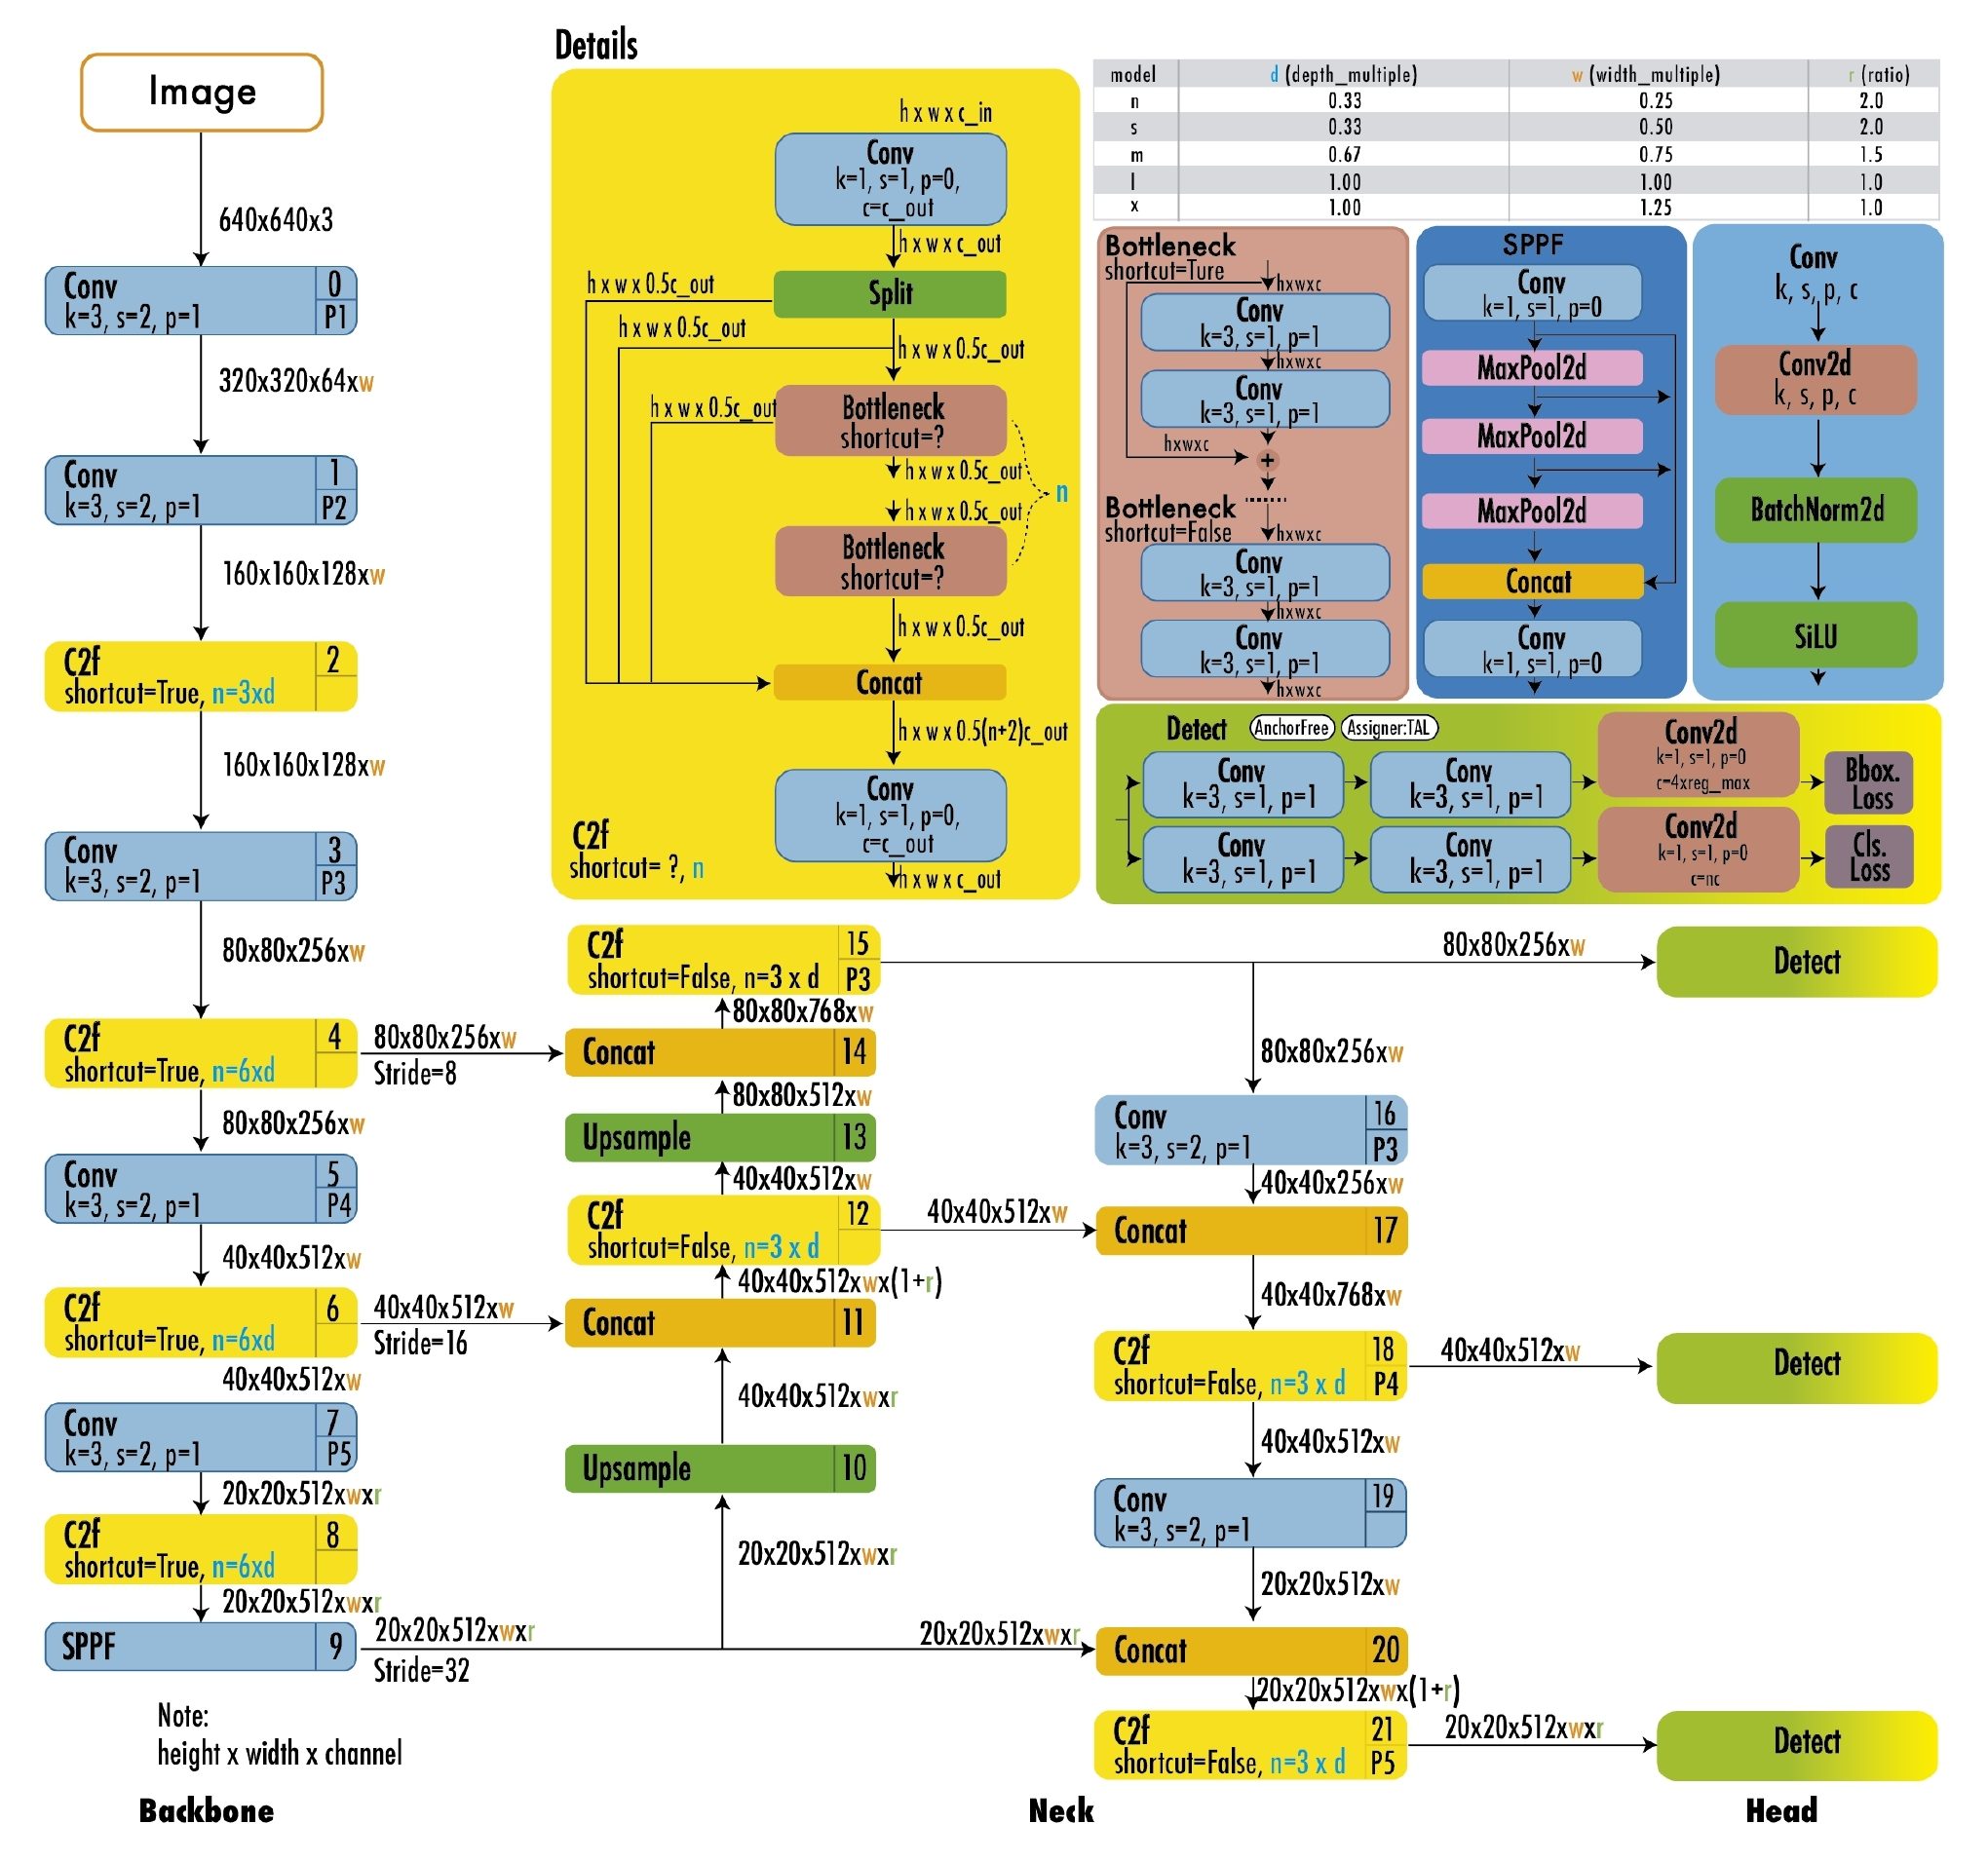
\includegraphics[scale=0.5]{gambar/YoloV8Architecture.jpg}

  % Ubah dengan keterangan gambar yang diinginkan
  \caption{Arsitektur YOLOv8.}
  \label{fig:Arsitektur Yolov8}
\end{figure}

Pada Gambar 2.1 merupakan gambar detail Arsitektur Yolov8.YOLOv8 menggunakan backbone yang serupa dengan YOLOv5 dengan beberapa perubahan pada CSPLayer, yang kini disebut modul C2f. Modul C2f (\emph{cross-stage partial bottleneck with two convolutions}) menggabungkan fitur tingkat tinggi dengan informasi kontekstual untuk meningkatkan akurasi deteksi.

YOLOv8 menggunakan model \emph{anchor-free} dengan \emph{decoupled head} untuk memproses tugas klasifikasi , dan regresi secara independen. Desain ini memungkinkan setiap cabang untuk fokus pada tugasnya dan meningkatkan akurasi model secara keseluruhan. Di output layer dari YOLOv8, mereka menggunakan fungsi aktivasi sigmoid untuk objectness score, yang mewakili probabilitas bahwa \emph{bounding box} mengandung suatu objek. Model ini menggunakan fungsi softmax untuk \emph{class probabilities}, yang mewakili probabilitas objek yang termasuk dalam setiap kelas yang mungkin.

YOLOv8 menggunakan \emph{loss functions} CIoU dan DFL untuk \emph{bounding box loss} dan \emph{binary cross-entropy} untuk \emph{classification loss}. Loss ini telah meningkatkan kinerja \emph{object detection}, terutama saat berhadapan dengan objek yang lebih kecil.

YOLOv8 juga menyediakan semantic \emph{segmentation model} yang disebut YOLOv8-Seg model. Backbone adalah CSPDarknet53 \emph{feature extractor}, diikuti oleh modul C2f bukan traditional YOLO neck architecture. Modul C2f diikuti oleh dua segmentation heads, yang belajar memprediksi semantic \emph{segmentation masks} untuk input image. Model ini memiliki \emph{detection heads} yang mirip dengan YOLOv8, terdiri dari lima detection modules dan prediction layer. YOLOv8-Seg model telah mencapai \emph{state-of-the-art results} pada berbagai \emph{object detection} dan \emph{semantic segmentation benchmarks} sambil menjaga \emph{high speed} dan efisiensi.

YOLOv8 dapat dijalankan dari \emph{command line interface} (CLI), atau juga dapat dipasang sebagai PIP package. Selain itu, dilengkapi dengan berbagai integrations untuk labeling, training, dan deploying.

Nilai Evaluasi pada MS COCO dataset test-dev 2017, YOLOv8x mencapai AP sebesar 53.9\% dengan image size 640 pixels (dibandingkan dengan 50.7\% dari YOLOv5 pada size input yang sama) dengan speed 280 FPS pada NVIDIA A100 dan TensorRT.

\section{Pose Estimation}
Estimasi pose adalah tugas menggunakan model pembelajaran mesin (\emph{ML}) untuk memperkirakan pose seseorang dari gambar atau video dengan mengestimasi lokasi spasial sendi tubuh utama (titik kunci atau \emph{keypoints}). Estimasi pose merujuk pada teknik visi komputer yang mendeteksi sosok manusia dalam gambar dan video, sehingga seseorang dapat menentukan, misalnya, di mana siku seseorang muncul dalam gambar. Penting untuk menyadari bahwa estimasi pose hanya memperkirakan di mana sendi tubuh kunci berada dan tidak mengenali siapa yang ada dalam gambar atau video.\parencite{tensorflow2015-whitepaper}

Model estimasi pose mengambil gambar kamera yang telah diproses sebagai input dan mengeluarkan informasi tentang titik kunci. Titik kunci yang terdeteksi diindeks oleh ID bagian, dengan skor kepercayaan antara 0,0 dan 1,0. Skor kepercayaan menunjukkan probabilitas bahwa titik kunci ada di posisi tersebut.\parencite{tensorflow2015-whitepaper}

\section{MediaPipe}
MediaPipe adalah kerangka kerja untuk membangun pipa yang melakukan inferensi dari data sensorik apa pun. Dengan MediaPipe, pipa persepsi dapat dibangun sebagai graf dari komponen modular, termasuk inferensi model, algoritma pengolahan media, dan transformasi data, dll. Data sensorik seperti aliran audio dan video memasuki graf, dan deskripsi yang dirasakan seperti aliran lokalizasi objek dan landmark wajah keluar dari graf. MediaPipe dirancang untuk praktisi pembelajaran mesin (ML) (\emph{machine learning}), termasuk peneliti, mahasiswa, dan pengembang perangkat lunak, yang mengimplementasikan aplikasi ML yang siap produksi, menerbitkan kode yang menyertai karya penelitian, dan membangun prototipe teknologi. Kasus penggunaan utama untuk MediaPipe adalah prototipe cepat dari pipa persepsi dengan model inferensi dan komponen yang dapat digunakan kembali lainnya. MediaPipe juga memfasilitasi penyebaran teknologi persepsi ke dalam demo dan aplikasi di berbagai platform perangkat keras yang berbeda. MediaPipe memungkinkan peningkatan bertahap pada pipa persepsi melalui bahasa konfigurasi yang kaya dan alat evaluasi. \parencite{MediaPipe}

Memodifikasi aplikasi persepsi untuk menggabungkan langkah-langkah pemrosesan tambahan atau model inferensi dapat sulit, karena penggabungan berlebihan antar langkah. Selain itu, mengembangkan aplikasi yang sama untuk platform yang berbeda memakan waktu dan biasanya melibatkan pengoptimalan langkah inferensi dan pemrosesan untuk berjalan dengan benar dan efisien pada perangkat target.

MediaPipe mengatasi tantangan ini dengan mengabstraksi dan menghubungkan model persepsi individu ke dalam pipa yang dapat dipelihara. Semua langkah yang diperlukan untuk mengambil inferensi dari data sensorik dan mendapatkan hasil yang dirasakan ditentukan dalam konfigurasi pipa. Mudah untuk menggunakan kembali komponen MediaPipe dalam pipa yang berbeda di seluruh aplikasi berturut-turut karena komponen ini berbagi antarmuka umum yang berorientasi pada data seri waktu. Setiap pipa kemudian dapat berjalan dengan perilaku yang sama di berbagai platform, memungkinkan praktisi untuk mengembangkan aplikasi di stasiun kerja, dan kemudian menerapkannya di mobile, misalnya. \parencite{MediaPipe}

MediaPipe terdiri dari tiga bagian utama: kerangka kerja untuk inferensi dari data sensorik, seperangkat alat untuk evaluasi kinerja, dan koleksi komponen inferensi dan pemrosesan yang dapat digunakan kembali yang disebut kalkulator.

\subsection{MediaPipe Pose}
MediaPipe Pose (MPP), sebuah kerangka kerja lintas platform sumber terbuka yang disediakan oleh Google, digunakan untuk mendapatkan perkiraan koordinat sendi manusia 2D dalam setiap bingkai gambar. MediaPipe Pose membangun pipa dan memproses data kognitif dalam bentuk video menggunakan pembelajaran mesin (\emph{machine learning} - ML). MPP menggunakan BlazePose yang mengekstrak 33 landmark 2D pada tubuh manusia seperti yang ditunjukkan pada Gambar 2.2. BlazePose adalah arsitektur pembelajaran mesin ringan yang mencapai kinerja real-time pada telepon seluler dan PC dengan inferensi CPU. Ketika menggunakan koordinat yang dinormalisasi untuk estimasi pose, rasio invers harus dikalikan dengan nilai piksel sumbu-y. \parencite{MediapipePose}

% Contoh input gambar
\begin{figure}[H]
  \centering

  % Ubah dengan nama file gambar dan ukuran yang akan digunakan
  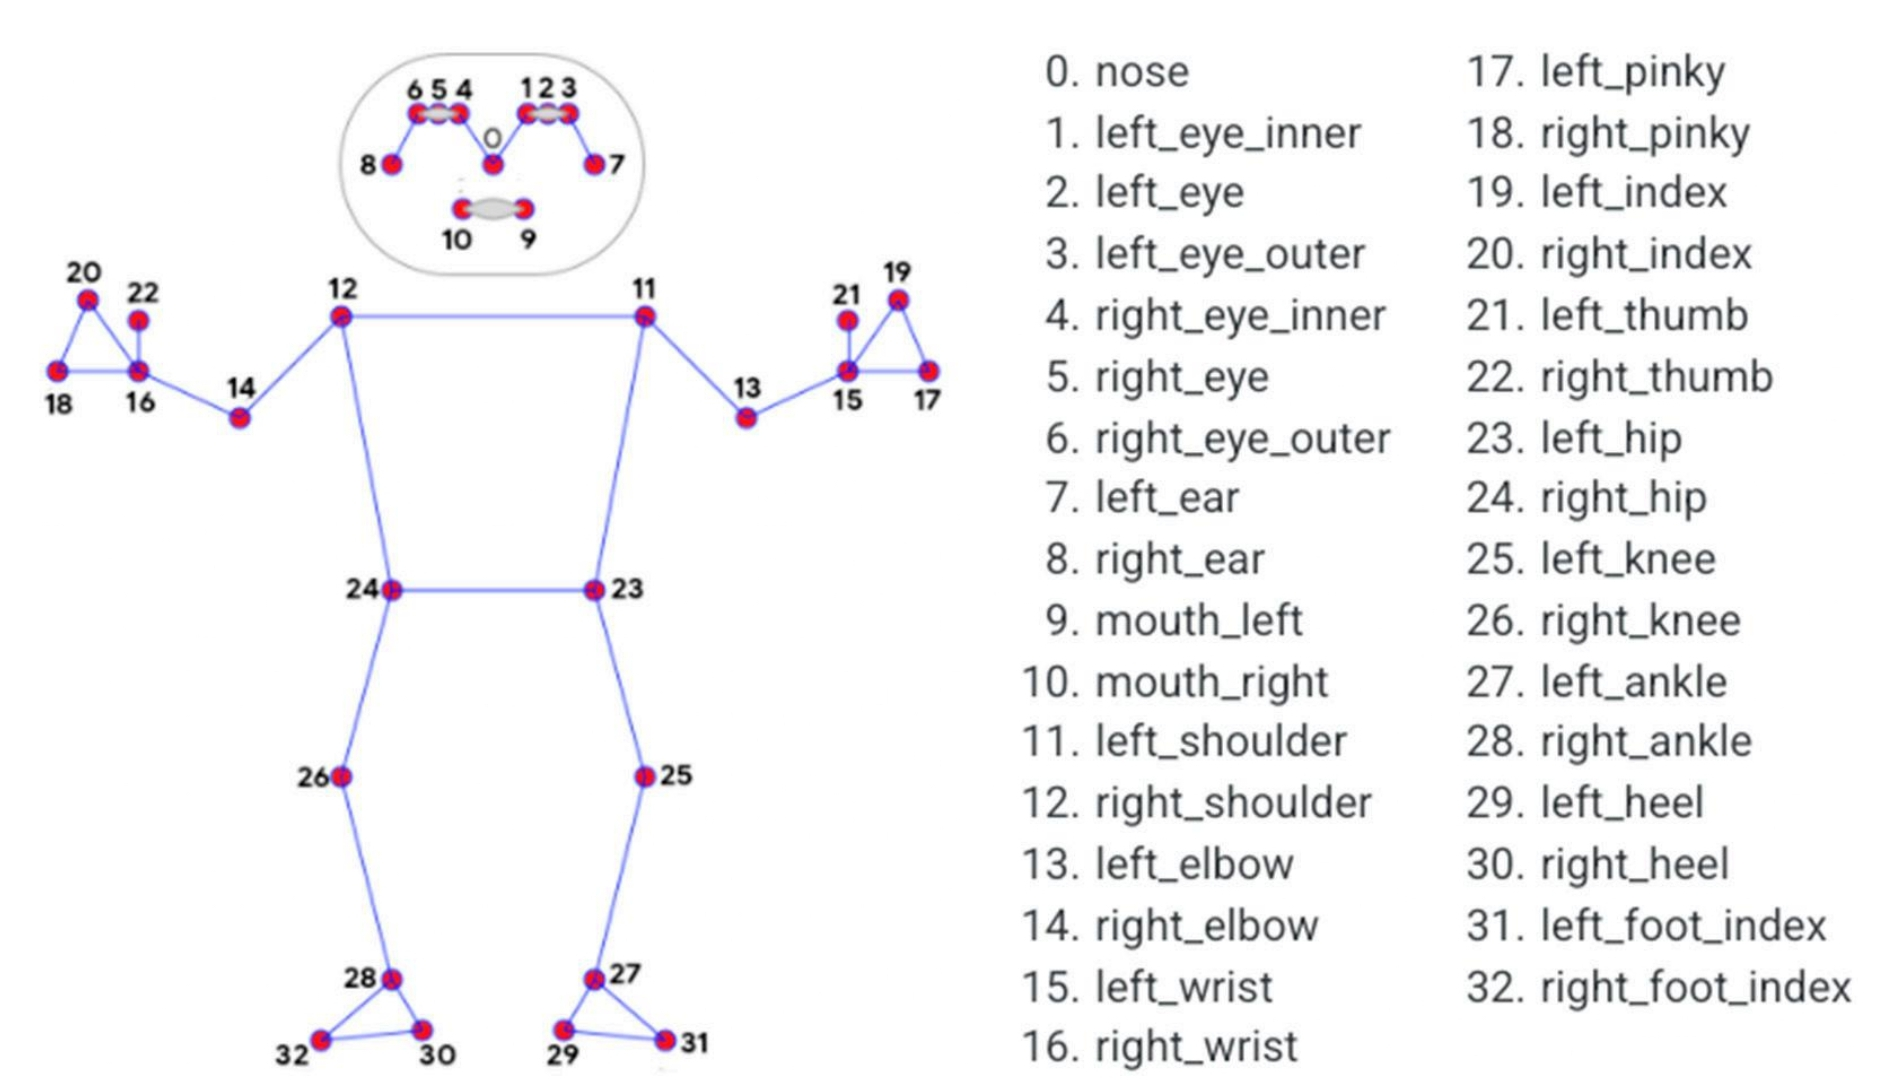
\includegraphics[scale=0.6]{gambar/mp_pose.jpg}

  % Ubah dengan keterangan gambar yang diinginkan
  \caption{Pose MediaPipe}
  \label{fig:Pose MediaPipe}
\end{figure}

\section{Classification Performance}
Dalam melakukan proses pengklasifikasian, diperlukan perhitungan efektifitas model yang telah dibuat berdasarkan beberapa pengukuran menggunakan set data pengetesan. Dalam hal ini, \emph{confusion matrix} merupakan salah satu perhitungan yang sering digunakan dalam kasus pengklasifikasian.

\emph{Confusion matrix} merupakan salah satu pengukuran yang paling mudah dilakukan dalam mencari nilai tingkat kebenaran dan juga akurasi dari model. \emph{Confusion matrix} adalah sebuah tabel berbentuk dua dimensi yang terdiri dari data aktual dan data prediksi yang masing-masing memiliki kelas. Data aktual terletak pada bagian kolom tabel, sedangkan data prediksi terletak pada bagian baris dari tabel. Gambar 2.3 merupakan representasi visual dari perhitungan confusion matrix.

% Contoh input gambar
\begin{figure}[H]
  \centering

  % Ubah dengan nama file gambar dan ukuran yang akan digunakan
  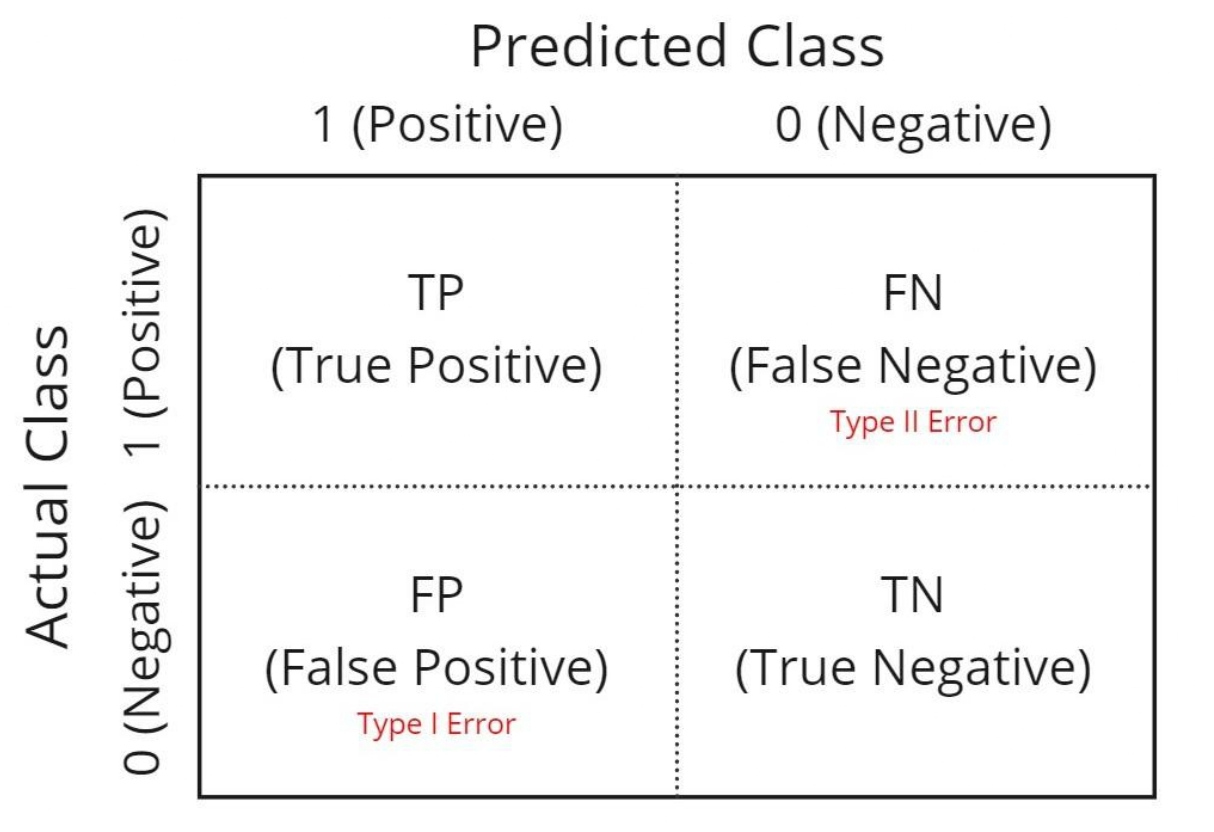
\includegraphics[scale=0.6]{gambar/halaman 37_page-0001 (1).jpg}

  % Ubah dengan keterangan gambar yang diinginkan
  \caption{Confusion Matrix}
  \label{fig:Confusion Matrix}
\end{figure}

\section{Evaluation Metrics}
\label{sec:gravitasi}
Penggunaan metrik evaluasi dalam konteks Deteksi Objek adalah sangat penting, karena ini berperan sebagai dasar kritis untuk membandingkan efektivitas berbagai algoritma dan skenario yang berbeda. Evaluasi yang teliti memungkinkan para peneliti untuk membuat perbandingan yang akurat antara berbagai teknik deteksi objek, serta menilai seberapa tepat tingkat keakuratan yang dicapai. Ini menjadi sangat vital dalam memilih algoritma yang paling cocok untuk tugas deteksi spesifik. Metrik seperti akurasi, presisi, dan recall adalah kunci dalam mengevaluasi seberapa efektif suatu model dalam mendeteksi dan mengidentifikasi objek dengan benar. Metrik-metrik ini penting untuk diimplementasikan demi menentukan model yang paling efisien.

Lebih lanjut, analisis akurasi memberikan wawasan kuantitatif yang signifikan mengenai kinerja algoritma deteksi objek, memberikan detail lebih lanjut mengenai kemampuan algoritma dalam menghasilkan deteksi yang akurat. Mengenali kesalahan melalui metrik evaluasi adalah langkah kritis dalam penelitian deteksi, seperti dalam kasus deteksi asap yang kami teliti. Langkah ini memfasilitasi identifikasi dan pemahaman tentang potensi kesalahan dalam algoritma, yang dapat membuka jalan untuk perbaikan dan peningkatan metode deteksi. Selanjutnya, metrik evaluasi juga mendukung pengoptimalan hiperparameter algoritma.

Dalam konteks penelitian ini, berbagai metrik evaluasi telah diterapkan, termasuk presisi, recall, dan Mean Average Precision (mAP). Dengan menggabungkan metode evaluasi ini, penelitian bertujuan untuk menyajikan analisis komprehensif mengenai kinerja dari algoritma deteksi objek yang ditinjau. Adapaun penjelasan konsep sederhana mengenai metrik evaluasi yang akan dijabarkan sebagai berikut :

\subsubsection*{1. Precision}
Precision merupakan rasio dimana TP (true positive) dimana jumlah positif benar dan FP (false positive) jumlah positif palsu sebagai metrik evaluasi dalam konteks machine learning, memberikan ukuran terhadap rasio prediksi positif yang tepat dibandingkan dengan seluruh prediksi positif yang diberikan oleh model. Dengan kata lain, precision 19 memberikan wawasan seberapa akurat model dalam membuat prediksi positif. Lebih rinci, precision mencerminkan seberapa sering model berhasil mengklasifikasikan instance sebagai positif dengan benar dalam keseluruhan dataset. Nilai precision dapat mengindikasikan sejauh mana model mampu memberikan prediksi yang benar dalam konteks positif. Rentang nilai precision berada antara 0 dan 1, di mana nilai 1 menunjukkan bahwa semua prediksi positif model adalah benar, sementara nilai 0 menunjukkan bahwa tidak ada prediksi positif yang benar.

\begin{equation}
    \frac{TP}{TP+FP}
\end{equation}

Pada persamaan diatas menyajikan perbandingan antara prediksi positif yang tepat dengan total prediksi positif yang diberikan oleh model, memberikan pandangan yang lebih mendalam terkait kemampuan model dalam menghasilkan hasil yang benar dalam kategori yang diinginkan

\subsubsection*{2. Recall}
Recall merupakan metrik yang digunakan untuk mengukur rasio dari data positif yangbenar yang ditemukan dari seluruh data positif. Recall memberikan informasi tentang seberapa baik model machine learning menemukan semua data positif. Nilai recall berkisar antara 0 dan 1. Recall yang tinggi menunjukan bahwa kelas yang dikenali dengan benar banyak, atau false negative yang didapatkan sedikit. Rumus dari recall dapat dilihat pada persamaan dibawah

\begin{equation}
    \frac{TP}{TP+FN}
\end{equation}

Recall merupakan rasio dimana TP (true positif ) adalah jumlah positif benar dan FN (false negative) jumlah negatif palsu

\subsubsection*{3. Mean Average Precision (mAP}
Mean Average Precision (mAP) adalah sebuah metrik akurasi yang dihasilkan dari menghitung rata-rata dari Average Precision (AP) atau presisi rata-rata. AP sendiri diperoleh melalui perhitungan precision dan recall. Oleh karena itu, mAP dapat dianggap sebagai metrik evaluasi yang sangat informatif dalam mengevaluasi kinerja suatu sistem.

\begin{equation}
    AP=\sum ((Recall_{n+1}-Recall_{n})\times Precision_{interp}\times Recall_{n+1})
\end{equation}
\begin{equation}
    mAP=\frac{1}{n}\sum_{n}^{i=1}AP_{i}
\end{equation}

\section{Intersection over Union (IoU)}
\label{subsec:hukumnewton}

Intersection over Union, atau IoU, adalah metrik yang digunakan untuk mengevaluasi keakuratan posisi objek yang dideteksi oleh model dalam pemrosesan gambar. Prinsipnya adalah dengan menghitung area persinggungan antara kotak deteksi yang dihasilkan oleh model dengan kotak referensi yang merupakan standar emas atau Ground Truth. Rasio ini didapat dengan membandingkan area irisan kedua kotak tersebut terhadap keseluruhan area yang mereka cakup secara bersamaan. Jika kita membayangkan kedua kotak tersebut sebagai satu kesatuan, maka IoU memberikan kita sebuah skor yang mengukur seberapa baik model kita dalam memprediksi lokasi objek sebenarnya. Semakin besar area persinggungan relatif terhadap total area gabungan, semakin tinggi nilai IoU, yang menandakan keakuratan prediksi yang lebih baik. Secara Sistematis, hal ini dituliskan sebagai :

% Contoh pembuatan persamaan
\begin{equation}
IntersectionoverUnion(IoU) = \frac{\left |A\bigcap B  \right |}{\left | A\bigcup B \right |}.
\end{equation}

IoU, atau Intersection over Union, merupakan metode penilaian yang mengukur efektivitas model deteksi objek dengan membandingkan area overlap antara prediksi model dan posisi objek aktual. Skala nilai IoU berada antara 0 hingga 1, di mana nilai yang lebih dekat ke 1 menandakan prediksi yang sangat akurat terhadap objek sebenarnya. Nilai IoU yang lebih tinggi menunjukkan bahwa model tersebut lebih tepat dalam mengidentifikasi dan menentukan lokasi objek.

Dalam skenario penelitian, misalnya pengenalan otomatis seekor hewan dalam sebuah gambar, model pembelajaran mendalam akan menciptakan sebuah kotak pembatas sebagai prediksi lokasi hewan tersebut. Kotak pembatas ini lalu dibandingkan dengan kotak kebenaran dasar—area yang telah ditentukan secara manual sebagai lokasi sebenarnya dari hewan dalam gambar. IoU kemudian dihitung untuk menilai seberapa baik kotak prediksi menutupi kotak kebenaran dasar, dengan mempertimbangkan area bersama dan area gabungan dari kedua kotak tersebut.

Dengan demikian, IoU berfungsi sebagai alat ukur yang penting dalam mengevaluasi kemampuan sebuah model deteksi objek untuk secara akurat menentukan posisi objek dalam berbagai kondisi, seperti variasi ukuran, orientasi, dan konteks objek dalam gambar. Sebuah nilai IoU yang tinggi menunjukkan bahwa model tersebut dapat diandalkan dalam mendeteksi dan mengidentifikasi objek dengan presisi yang tinggi.

\begin{figure}[H]
  \centering

  % Ubah dengan nama file gambar dan ukuran yang akan digunakan
  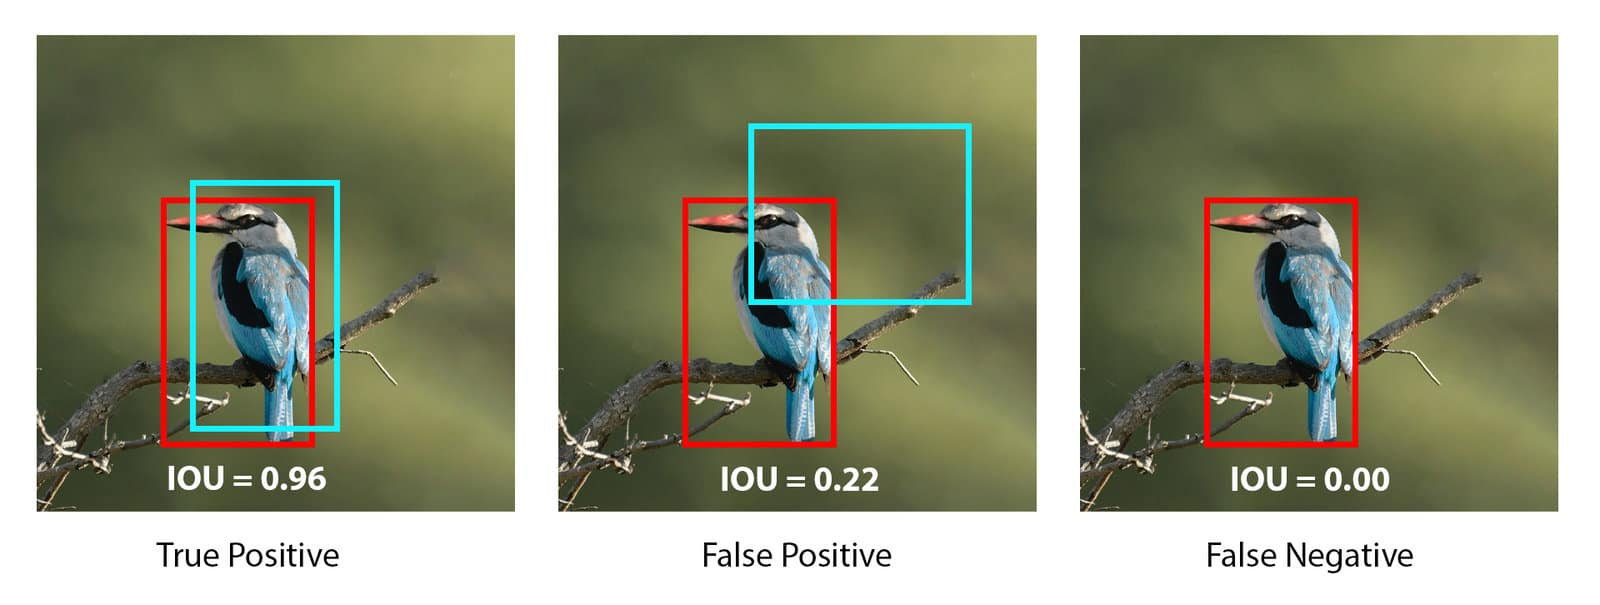
\includegraphics[scale=0.3]{gambar/Perbandingan nilai iou.jpg}

  % Ubah dengan keterangan gambar yang diinginkan
  \caption{Perbandingan Performa Berdasarkan IoU}
  \label{fig:roketluarangkasa}
\end{figure}

IoU menawarkan metode kuantitatif untuk mengevaluasi seberapa akurat model dalam mengenali dan menandai objek dalam gambar. Dalam proses pelatihan, nilai IoU minimal yang ditetapkan memungkinkan penetapan batas bagi kotak prediksi untuk dianggap cocok dengan deteksi yang benar, memfasilitasi penyesuaian antara tingkat akurasi deteksi dan insiden false positif. Penentuan batas IoU tidak bersifat tetap dan dapat disesuaikan, dengan 0,5 yang menjadi standar patokan awal. Kotak prediksi dengan IoU minimal 0,5 terhadap deteksi positif dianggap valid. Penyesuaian ambang nilai ini mempengaruhi balance antara presisi dan daya tangkap, dengan peningkatan nilai ambang cenderung mengurangi kesalahan positif namun berpotensi mengabaikan beberapa deteksi valid.

Penggunaan nilai kebenaran dasar dalam IoU merupakan perbandingan standar antara prediksi dan kondisi aktual objek yang diidentifikasi. Penandaan kotak kebenaran dasar, dilakukan secara manual oleh pakar, menentukan batas pasti objek dalam gambar. Skor IoU yang dihasilkan dari perbandingan antara prediksi model dengan batas ini memberikan wawasan terhadap efektivitas model dalam deteksi objek. Dataset kebenaran dasar, yang meliputi kotak pembatas yang ditandai secara manual, menjadi kunci dalam proses evaluasi ini, memberikan dasar objektif untuk mengukur kinerja algoritme deteksi objek.

Dengan demikian, IoU bukan hanya sekedar metrik evaluasi tetapi juga alat penting dalam pengembangan dan penyesuaian model deteksi objek, memastikan bahwa model dapat diandalkan dan akurat dalam berbagai kondisi dan skenario pengujian. \parencite{shah2023intersection}

\section{Single Board Computer (SBC)}
Single Board Computer (SBC) adalah komputer lengkap yang dibangun pada satu papan sirkuit tunggal, dengan mikroprosesor, memori, input/output (I/O), dan fitur lain yang diperlukan untuk fungsi komputer penuh. SBC dirancang untuk menjadi kompak dan efisien, sering digunakan dalam aplikasi tertanam, perangkat IoT, dan proyek-proyek pengembangan karena kemudahan penggunaan dan ukurannya yang kecil. SBC menyediakan platform yang ideal untuk pengembangan prototipe dan implementasi sistem kontrol dalam berbagai aplikasi, termasuk kursi roda otonom.

Dalam perkembangan teknologi , penggunaan Single Board Computer (SBC) seperti Intel NUC, NVIDIA Jetson Nano Developer Kit dan Rasberry Pi 4 telah berperan sangat penting terutama dalam Deteksi Real-time. Kecepatan yang ditawarkan SBC dalam memproses data dari sensor dan kamera  , serta menjalankan model visi komputer berbasis deep learning membuat alat ini menjadi standar dalam memilih alat untuk implementasi model Deteksi secara real time. Selain itu SBC juga biasanya dilengkapi dengan konektifitas yang sangat baik sehingga dapat terhubung dengan banyak IO. \parencite{Elliot_Residing}

\section{Roboflow}
RoboFlow adalah platform yang mendukung pengembangan dan penyebaran aplikasi visi komputer dengan menyediakan alat-alat canggih untuk manajemen dan peningkatan dataset. Platform ini dirancang untuk memudahkan pengolahan, analisis, dan augmentasi data visual, sehingga mempercepat siklus pengembangan dan peningkatan model pembelajaran mesin.

\begin{figure}[H]
  \centering

  % Ubah dengan nama file gambar dan ukuran yang akan digunakan
  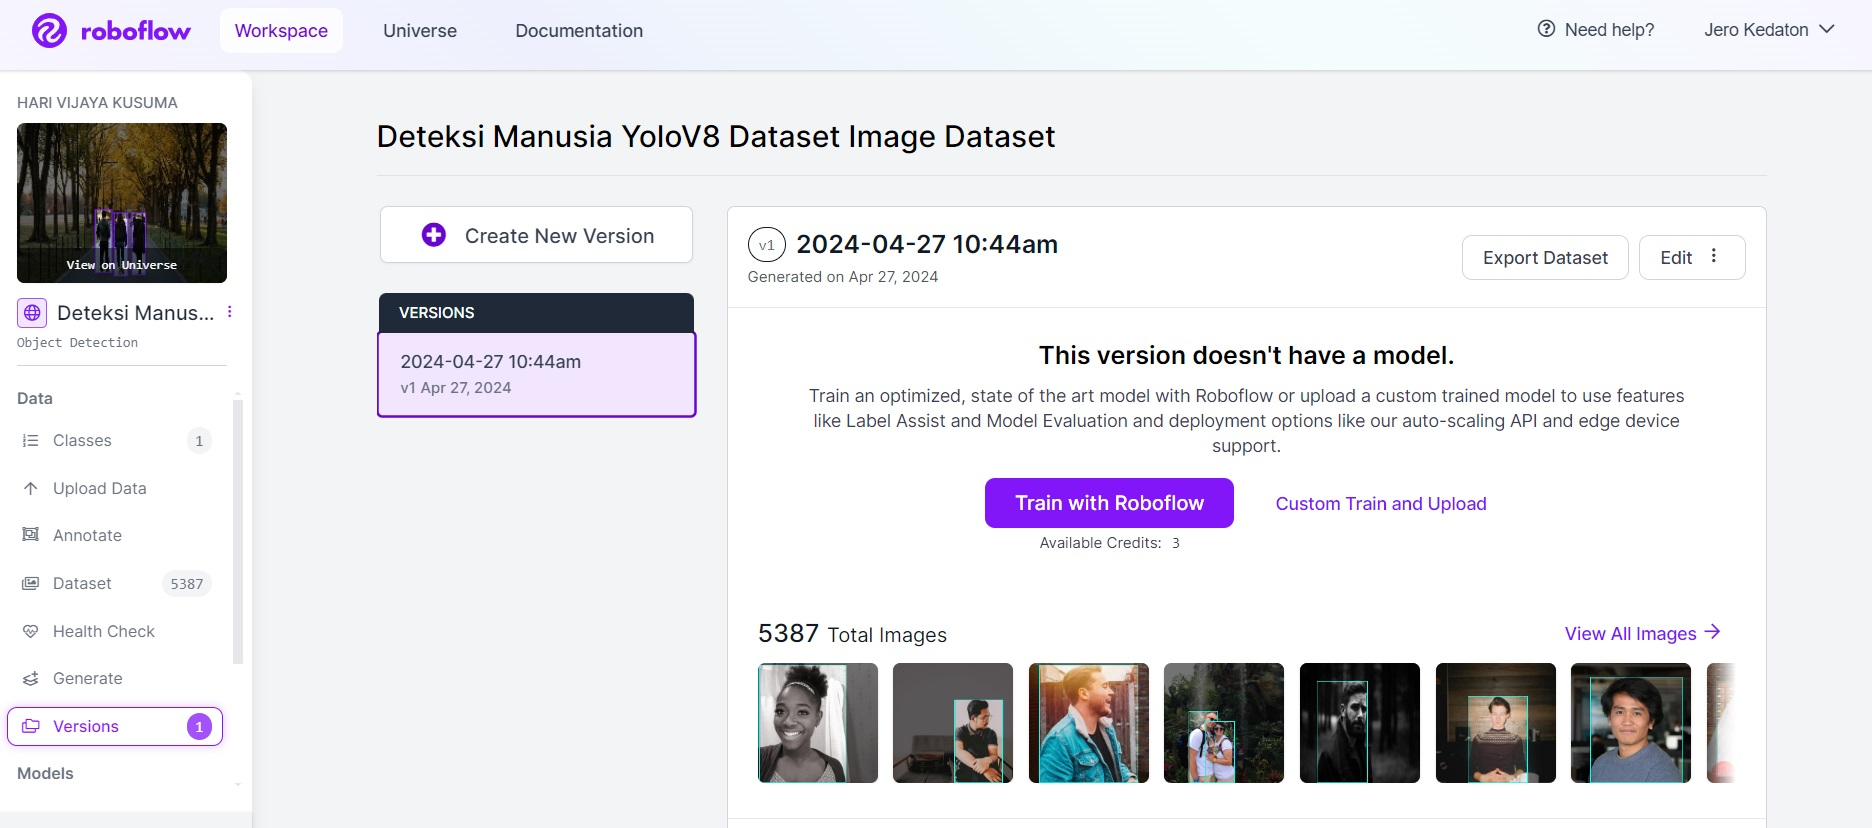
\includegraphics[scale=0.3]{gambar/roboflow.jpg}

  % Ubah dengan keterangan gambar yang diinginkan
  \caption{Interface Roboflow}
  \label{fig:roboflow}
\end{figure}

RoboFlow menyediakan serangkaian fungsi yang membantu dalam proses pengembangan model visi komputer, termasuk:
\begin{itemize}
    \item Annotasi Data : RoboFlow memungkinkan pengguna untuk menandai gambar dengan alat bantu yang intuitif, mempercepat proses pembuatan label untuk dataset.
    \item Augmentasi Data: Melalui augmentasi data, RoboFlow dapat secara otomatis memodifikasi gambar dalam dataset untuk menciptakan variasi, yang membantu dalam meningkatkan robustness model yang dilatih.
    \item Konversi Format Data: Platform ini mendukung konversi antara berbagai format dataset yang populer, memudahkan pengguna dalam mempersiapkan data untuk berbagai jenis algoritma pembelajaran mesin.
    \item Pemisahan Dataset: RoboFlow menyediakan fungsi untuk membagi dataset menjadi set pelatihan, validasi, dan pengujian, yang merupakan langkah penting dalam validasi model.
\end{itemize}
RoboFlow menawarkan integrasi yang mulus dengan banyak kerangka kerja pembelajaran mesin populer seperti TensorFlow, PyTorch, dan YOLO. Integrasi ini memungkinkan pengembang:
\begin{itemize}
    \item Ekspor Data: Pengguna dapat dengan mudah mengekspor dataset mereka dalam format yang siap digunakan oleh kerangka kerja pembelajaran mesin pilihan mereka.
    \item Pelatihan Model: Platform ini menyediakan alat yang memungkinkan pengguna untuk langsung melatih model mereka menggunakan dataset yang telah disiapkan dan dioptimalkan.
    \item Evaluasi Model: RoboFlow menyediakan metrik untuk mengukur kinerja model, membantu pengguna memahami efektivitas model mereka dan membuat penyesuaian yang diperlukan.
\end{itemize}

\section{Intel NUC}
Intel NUC (Next Unit of Computing) adalah solusi komputasi yang kompak dan kuat yang dirancang oleh Intel untuk memenuhi berbagai kebutuhan komputasi, mulai dari hiburan rumah hingga gaming dan tugas profesional. Intel NUC dengan fitur prosesor Intel Core generasi dalam form factor kompak 4x4 inci. Dirancang untuk menawarkan kombinasi ukuran, kinerja, keberlanjutan, dan keandalan yang dibutuhkan oleh bisnis modern. Intel NCU model tertentu juga menyertakan teknologi Intel vPro® Enterprise dengan keamanan yang ditingkatkan. Mini PC ini dapat diupgrade dan diperbaiki, menjadikannya pilihan serbaguna untuk berbagai aplikasi bisnis termasuk komputasi klien, komputasi edge, dan digital singage.

\begin{figure}[H]
  \centering

  % Ubah dengan nama file gambar dan ukuran yang akan digunakan
  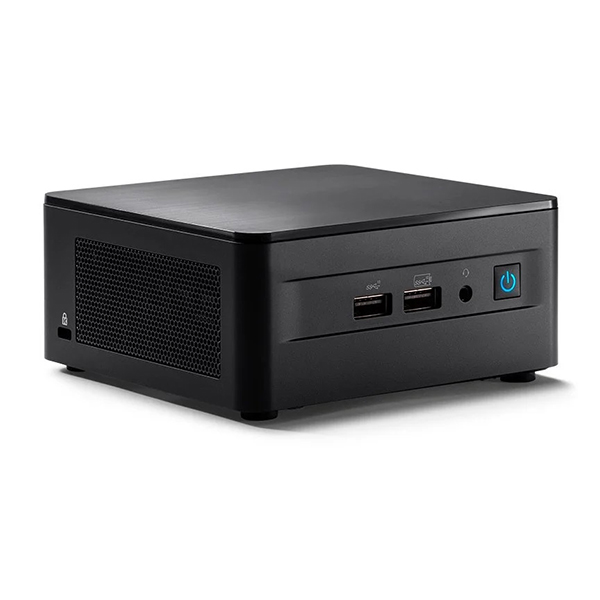
\includegraphics[scale=0.3]{gambar/INTEL-NUC-RNUC12WSHI30000-1.jpg}

  % Ubah dengan keterangan gambar yang diinginkan
  \caption{Gambar Intel NUC}
  \label{fig:roketluarangkasa}
\end{figure}

\section{ESP32 Devkit V1}

ESP32 Devkit V1 adalah salah satu development board yang dibuat oleh DOIT untuk menjalankan modul ESP-WROOM-32 buatan Espressif. ESP32 Devkit dikenal dengan Development board yang kaya fitur dengan konektivitas Wi-Fi dan Bluetooth terintegrasi untuk beragam aplikasi. Devkit ini memiliki banyak pin yang memungkinkannya untuk diprogram dengan banyak tugas.

\begin{figure}[H]
  \centering

  % Ubah dengan nama file gambar dan ukuran yang akan digunakan
  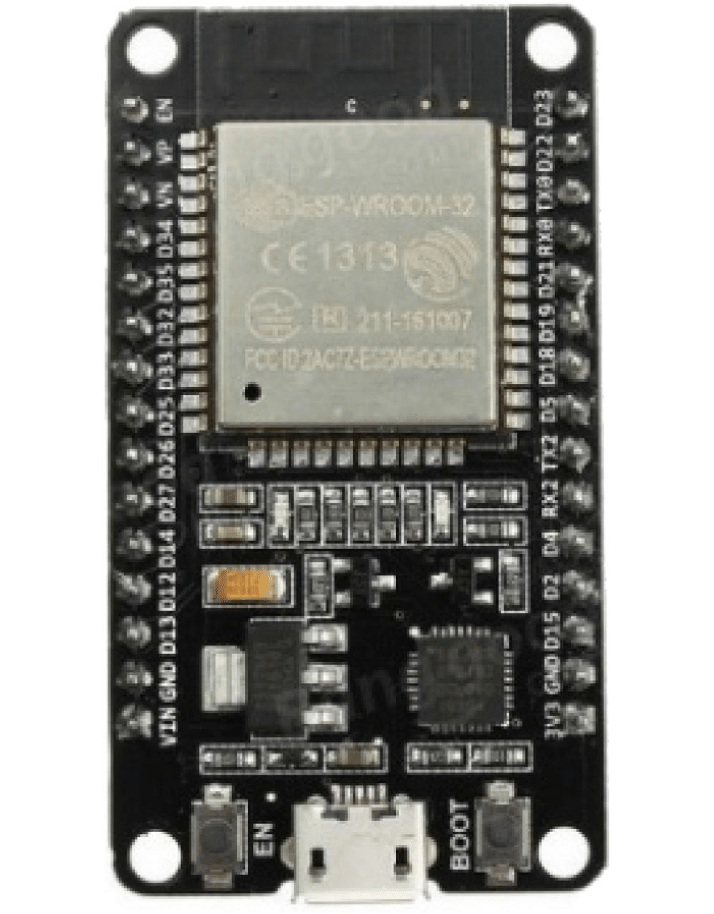
\includegraphics[scale=0.2]{gambar/The-ESP32-DEVKIT-V1-board-used-as-controller.png}

  % Ubah dengan keterangan gambar yang diinginkan
  \caption{Gambar ESP32 Devkit V1}
  \label{fig:roketluarangkasa}
\end{figure}

\section{Motor Driver H-Bridge}

Driver motor H-Bridge adalah rangkaian elektronik yang digunakan untuk mengontrol arah dan kecepatan motor DC. Cara kerjanya berdasarkan empat switch yang membentuk jembatan H (H-Bridge), yang mana dengan mengatur pembukaan dan penutupan switch-switch ini, kita dapat mengatur arah arus yang mengalir ke motor. Dengan demikian, kita bisa mengubah arah putaran motor DC. Driver Motor H-Bridge tersusun oleh sekumpulan transistor yang berfungsi sebagai pengendali motor, terutama yang memerlukan arus serta tegangan yang cukup besar. selain itu, Rangkaian H-Bridge juga dapat memberikan fungsi pengereman pada motor dengan menghubungkan kedua terminal motor sehingga motor dapat berhenti lebih cepat. \parencite{fibrianianalisis}

\begin{figure}[H]
  \centering

  % Ubah dengan nama file gambar dan ukuran yang akan digunakan
  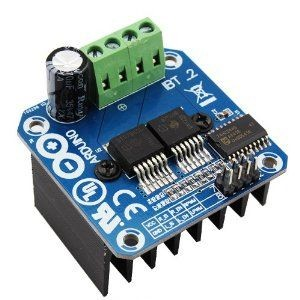
\includegraphics[scale=0.3]{gambar/Motor Driver H - bridge Bts.jpg}

  % Ubah dengan keterangan gambar yang diinginkan
  \caption{Gambar Motor Driver H-Bridge}
  \label{fig:roketluarangkasa}
\end{figure}

\section{Kursi Roda Elektrik KY-123}

Kursi roda bertenaga listrik merupakan alat bantu mobilitas yang terdiri dari struktur dasar kursi roda, sistem pengendalian gerak, mesin elektrik, dan modul baterai. Keunggulan alat ini terletak pada kemampuannya untuk dikendalikan dengan mudah dan nyaman, meminimalkan usaha fisik yang diperlukan pengguna dibandingkan dengan kursi roda manual. Ini sangat bermanfaat bagi individu dengan kondisi hemiplegia, memungkinkan pengoperasian dengan satu tangan. Selain itu, kursi roda elektrik ini juga memberikan solusi mobilitas yang lebih baik bagi lansia yang mengalami keterbatasan dalam bergerak.

\begin{figure}[H]
  \centering

  % Ubah dengan nama file gambar dan ukuran yang akan digunakan
  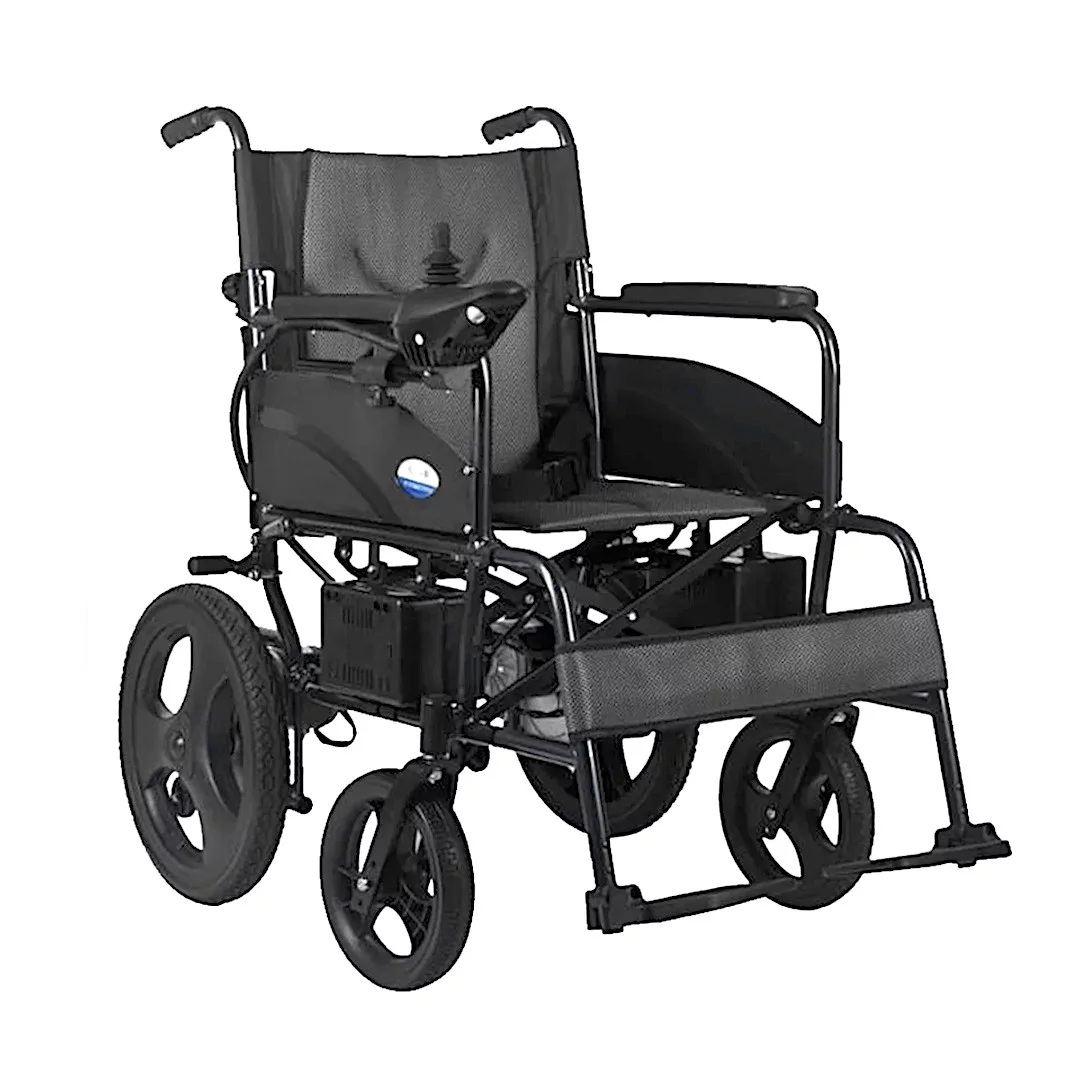
\includegraphics[scale=0.3]{gambar/Kursi Roda Elektrik Lipat OneHealth KY123 A.jpg}

  % Ubah dengan keterangan gambar yang diinginkan
  \caption{Gambar Kursi Roda Elektrik KY-123}
  \label{fig:roketluarangkasa}
\end{figure}


\cleardoublepage

% Bab 3 desain dan implementasi
\chapter{DESAIN DAN IMPLEMENTASI}
\label{chap:desainimplementasi}

% Ubah bagian-bagian berikut dengan isi dari desain dan implementasi
Penelitian ini dilakukan sesuai dengan desain sistem berikut beserta implementasinya. Desain sistem adalah konsep dari pembuatan dan perancangan infrastruktur dan kemudian diwujudkan dalam bentuk alur yang harus dikerjakan 
\section{Deskripsi Sistem}
\label{sec:deskripsisistem}
Penelitian dan pembuatan sistem ini diterapkan sesuai dengan desain dan implementasi pada bab ini. Desain sistem ini mencakup konsep pembuatan, perancangan, alur, dan implementasi infrastruktur yang dibuat dalam Blok Diagram. Desain dan penerapan diilustrasikan melalui penggunaan Gambar dan akan dijelaskan mulai dari pengumpulan data berupa citra, analisa dari model yang telah dibuat untuk mendeteksi objek Manusia, serta sistem yang menggunakan model tesebut seperti Gambar 3.1 berikut dan dirincikan pada tiap subbab.

\begin{figure}[H]
  \centering

  % Ubah dengan nama file gambar dan ukuran yang akan digunakan
  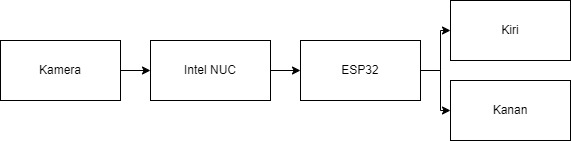
\includegraphics[scale=0.6]{gambar/hardware.jpg}

  % Ubah dengan keterangan gambar yang diinginkan
  \caption{Blok Diagram Hardware}
  \label{fig:roketluarangkasa}
\end{figure}
\subsection{Kamera}
Pada tugas akhir ini pendeteksian menggunakan data citra yang diolah untuk mendapatkan output berupa deteksi manusia yang akan dianalisa jaraknya. Kamera menjadi input utama untuk mendapatkan citra yang akan dipasangkan dalam kursi roda otonom.Posisi kamera yang digunakan harus berada pada posisi yang dapat menangkap citra manusia dengan jelas. Adapun kamera yang digunakan adalah kamera Logitech C920. 

Kamera Logitech C920 dilengkapi dengan lensa kaca Carl Zeiss dan sensor Gambar Full HD 1080p. Kamera ini juga mendukung video call dalam resolusi 720p yang berkualitas tinggi. Fitur autofocus otomatisnya memastikan bahwa Gambar tetap fokus bahkan ketika pengguna bergerak. Logitech C920 juga dilengkapi dengan dua mikrofon stereo yang dapat merespons suara dengan jelas dan natural, menghasilkan pengalaman audio yang memuaskan tanpa perlu penggunaan mikrofon eksternal. Dengan kombinasi fitur dan spesifikasi ini, Logitech C920 sudah lebih dari cukup untuk digunakan sebagai kamera untuk mendeteksi obstacle  yang hendak dideteksi.

\subsection{Intel NUC}
Intel NUC digunakan sebagai komputer pusat dalam kursi roda otonom untuk memproses citra dari kamera dan menjalankan algoritma deteksi objek. Data yang dihasilkan dari deteksi digunakan untuk mengambil keputusan navigasi. Misalnya, menghindari hambatan dan menentukan arah gerak. Perintah tersebut kemudian dikirim ke ESP32 yang mengontrol mekanisme penggerak kursi roda.

Penggunaan Intel NUC tidak langsung dapat menjalankan sistem yang dibuat, melainkan perlu diinstal library agar dapat menjalankan sistem yang telah dibuat.

\begin{lstlisting}
pip install opencv-python
pip install ultralytics
pip install mediapipe

\end{lstlisting}
opencv-python digunakan untuk menangkap dan memproses citra dari kamera. Ultralytics digunakan untuk menjalankan deteksi objek menggunakan model YOLOv8. Mediapipe digunakan untuk menampilkan landmark pada manusia
\subsection{ESP32}
Untuk dapat menggerakkan kursi roda maka perlu mengirimkan perintah ke kontroler kursi roda. ESP32 menjadi akan menerima input perintah dasar untuk menggerakkan kursi roda, seperti maju, kanan, kiri. Perintah ini kemudian akan digabungkan dengan kecepatan maksimal menjadi satu command atau paket data seperti ”Arah”. Berikut merupakan tabel kode instruksi kursi roda berdasarkan hasil deteksi \parencite{ekatama2024perancangan}

% Contoh pembuatan tabel
\begin{longtable}{|c|c|}
    \caption{Kode instruksi dari hasil klasifikasi}
    \label{tbl:kode-instruksi}\\
        \hline
        Klasifikasi Pose & Kode Instruksi \\ \hline
        \endfirsthead
        %
        \endhead
        %
        Kiri             & A              \\ \hline
        Maju             & B              \\ \hline
        Stop             & C              \\ \hline
        Mundur           & D              \\ \hline
        Kanan            & E              \\ \hline
\end{longtable}


Setelah variabel tersebut dimasukkan maka akan dikirim secara nirkabel. Dalam tugas akhir ini menggunakan wifi dengan ssid Haris-Acess-Point setelah terkoneksi.

Paket data yang telah dikirimkan melalui NUC akan diterima oleh ESP32 menggunakan WiFi. Saat diterima oleh ESP32, data tersebut akan menjalani serangkaian proses yang melibatkan pemecahan paket data dan penyesuaian sesuai dengan variabel yang telah ditentukan sebelumnya. Pemecahan paket data ini memungkinkan ESP32 untuk mendekomposisi informasi yang terkandung dalam setiap paket dan memastikan bahwa setiap variabel terpisah dengan akurat. Dengan demikian proses ini akan mengorganisir dan menyusun kembali informasi serta memastikan bahwa setiap variabel telah benar sesuai dengan nama variabel dan tipe data yang disediakan.

\subsection{Skematik Alat}

\begin{figure}[H]
  \centering

  % Ubah dengan nama file gambar dan ukuran yang akan digunakan
  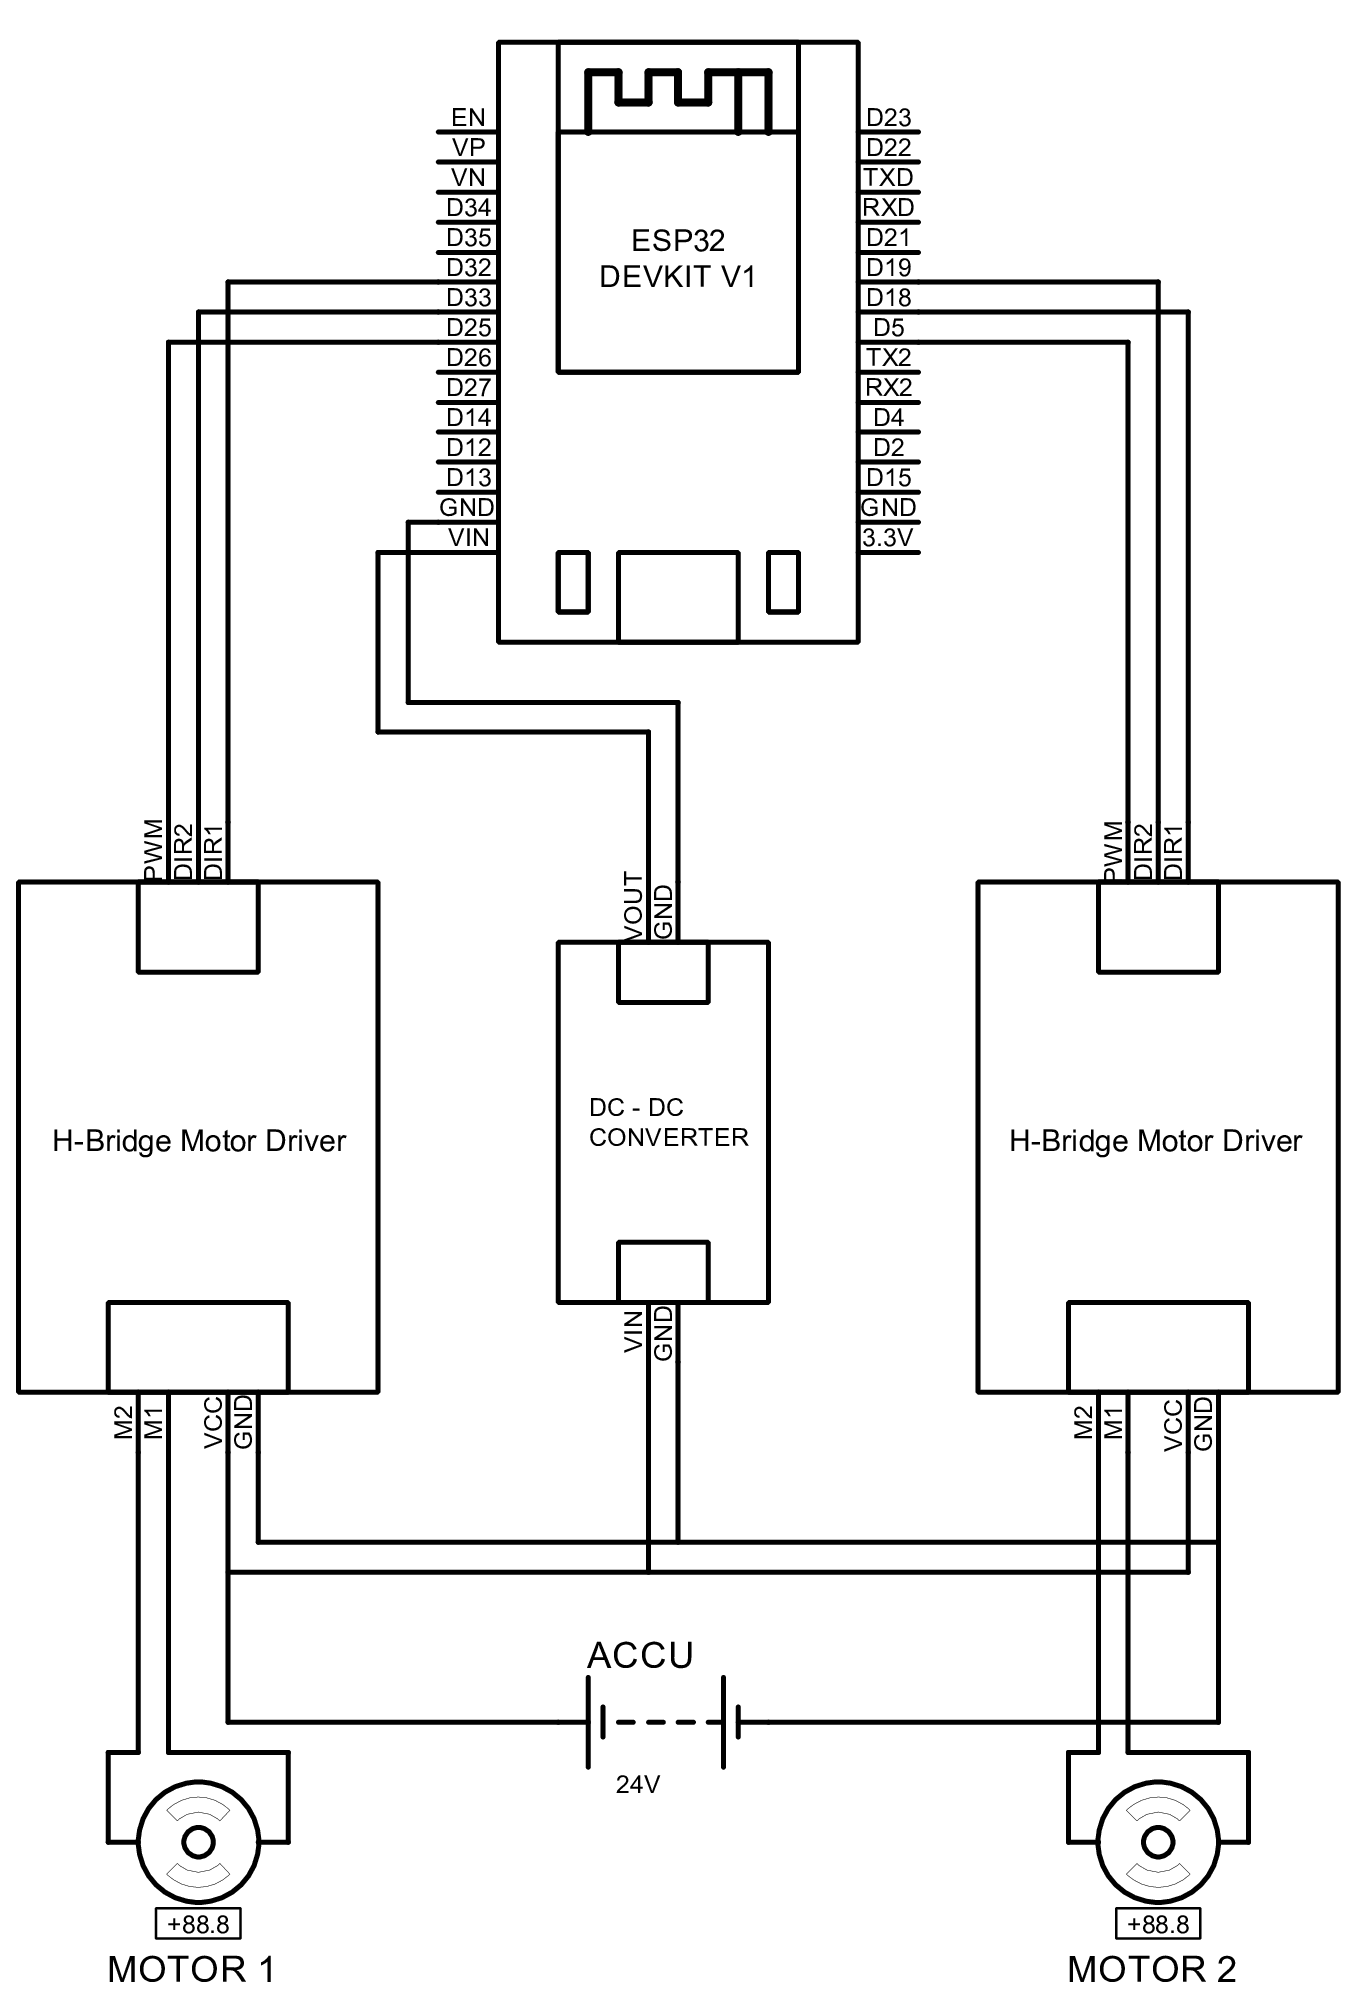
\includegraphics[scale=0.3]{gambar/Schematics.png}

  % Ubah dengan keterangan gambar yang diinginkan
  \caption{Skematik kontrol motor kursi roda}
  \label{fig:roketluarangkasa}
\end{figure}

Gambar menampilkan skema detail dari perangkat yang dibahas. Sistem ini menggunakan kamera yang terhubung ke NUC, yang berfungsi sebagai perangkat utama untuk pengambilan gambar objek. Ketika kamera berhasil menangkap gambar objek, data citra tersebut kemudian diproses oleh Laptop atau Jetson Nano. Di dalam sistem, terdapat model klasifikasi yang telah diprogram untuk menganalisis data citra ini secara detail. Hasil analisis ini sangat penting, sebab menjadi dasar dalam pembuatan kode instruksi yang akan dieksekusi oleh sistem.

Kode instruksi yang dihasilkan kemudian diintegrasikan dengan parameter kecepatan maksimal yang telah ditetapkan oleh pengguna. Integrasi antara kode instruksi tersebut kemudian dikemas dalam bentuk paket data yang digunakan untuk mengatur dan mengendalikan pergerakan kursi roda. Paket data ini selanjutnya ditransmisikan secara nirkabel, menggunakan teknologi WiFi, menuju modul ESP32 Devkit V1.

ESP32 memegang peranan kunci dalam mekanisme pengendalian motor kursi roda, berfungsi sebagai pusat pengendalian yang menerima paket data dari pengguna melalui koneksi nirkabel. Setelah menerima paket, ESP32 akan menguraikan paket data tersebut untuk menyesuaikan dengan variabel-variabel yang telah ditentukan. Proses dekripsi ini menghasilkan dua variabel utama yang akan diproses lebih lanjut oleh ESP32 untuk pengoperasian kursi roda.

Variabel utama pertama adalah variabel arah, yang memainkan peran kritis dalam menentukan arah gerakan motor-motor pada kursi roda, memastikan bahwa gerakan motor selaras dengan arah yang dikehendaki berdasarkan data yang telah dianalisis dan diterima, sehingga pergerakan kursi roda dapat dikontrol dengan aman dan efisien.\parencite{ekatama2024perancangan}


\section{Software}
Perancangan software dilakukan sesuai dengan alur yang akan dideskripsikan pada subbab ini. Perangangan ini akan dipresentasikan dengan blok diagram alur yang telah merepresentasikan alur perancangan software ini. Gambar blok diagram alur akan ditampilkan sebagai berikut :

\begin{figure}[H]
    \centering
    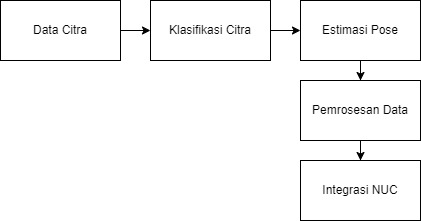
\includegraphics[scale = 0.6]{gambar/DIagram p.jpg}
    \caption{Diagram Blok Software}
    \label{fig:enter-label}
\end{figure}

\subsection{Pengumpulan Dataset citra
  \label{sec:Dataset Citra}}
Dalam pengembangan Tugas Akhir ini akan digunakan dataset citra berupa gambar, Dimana objek yang akan dideteksi pada gambar tersebut ialah Manusia yang fungsinya dalam tugas ini sebagai obstacle yang akan dihindari. citra manusia tersebut diambil melalui setiap frame citra pada video yang didapatkan menggunakan kamera webcam yang terhubung dengan komputer. Kemudian setiap citra yang didapatkan nantinya akan diproses untuk menentukan apakah terdapat manusia atau tidak pada citra tersebut. Dalam pendeteksian, nantinya proses ini terjadi secara real-time guna mendapatkan keseluruhan citra yang dibutuhkan untuk mengenali manusia atau tidak pada citra secara terus-menerus

\begin{figure}[H]
  \centering
  % Ubah dengan nama file gambar dan ukuran yang akan digunakan
  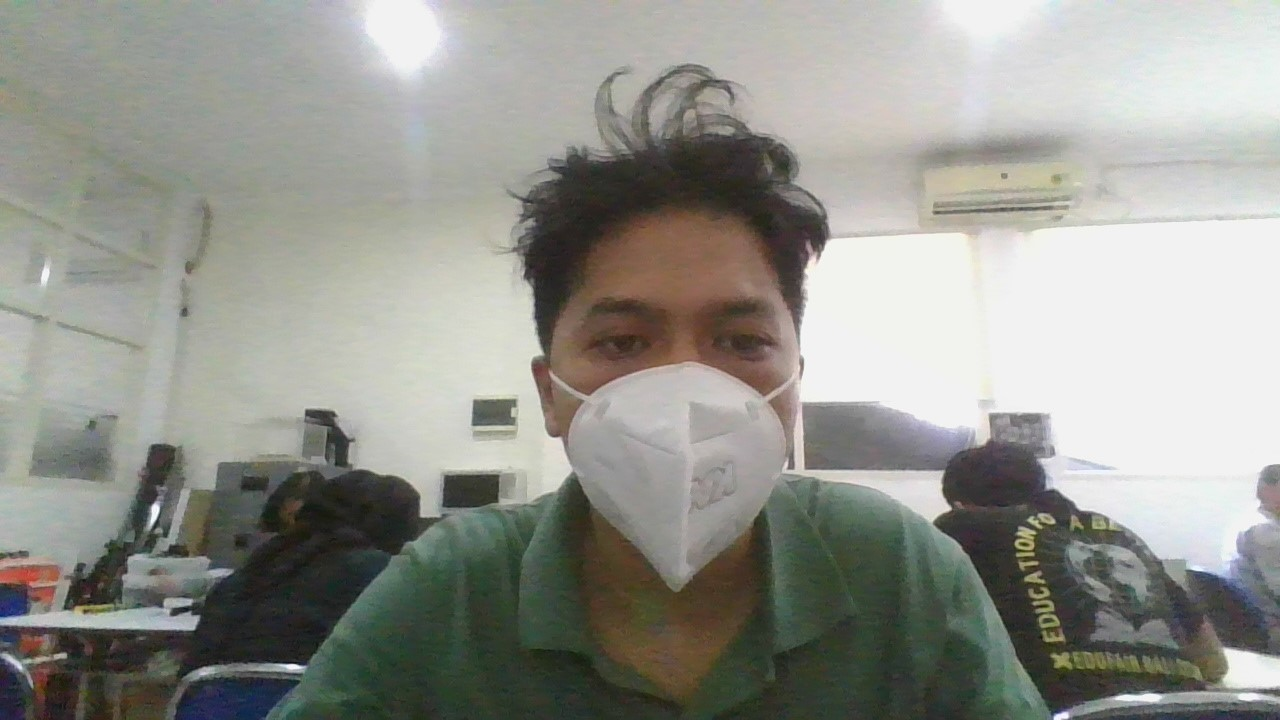
\includegraphics[scale=0.3]{gambar/WIN_20240319_17_11_26_Pro.jpg}
  % Ubah dengan keterangan gambar yang diinginkan
  \caption{Contoh Hasil data dari Citra.}
  \label{fig:Hasil Data dari Citra}
\end{figure}

Dengan menggunakan perangkat kamera yang terhubung dengan komputer, perangkat akan menghubungkan interaksi antara pengguna dengan komputer untuk mendapatkan frame citra pada video agar nantinya dapat diproses. Gambar 3.2 merupakan contoh hasil dari data citra yang didapatkan melalui perangkat kamera pada komputer. Dalam hal ini, karena yang ingin dikenali adalah manusia, maka citra gambar citra yang didapatkan harus memiliki objek manusia didalamnya.

\subsection{Labeling Menggunakan Roboflow}
Dataset citra yang sudah didapatkan selanjutnya akan melalui proses labeling dan augmentasi. Dimana Roboflow memiliki tools yang mumpuni dalam melakukan labeling. Dimana terdapat beberapa proses yang akan dilakukan yaitu, import dataset, pelabelan dataset dan augmentasi dataset

\begin{figure}[H]
  \centering
  % Ubah dengan nama file gambar dan ukuran yang akan digunakan
  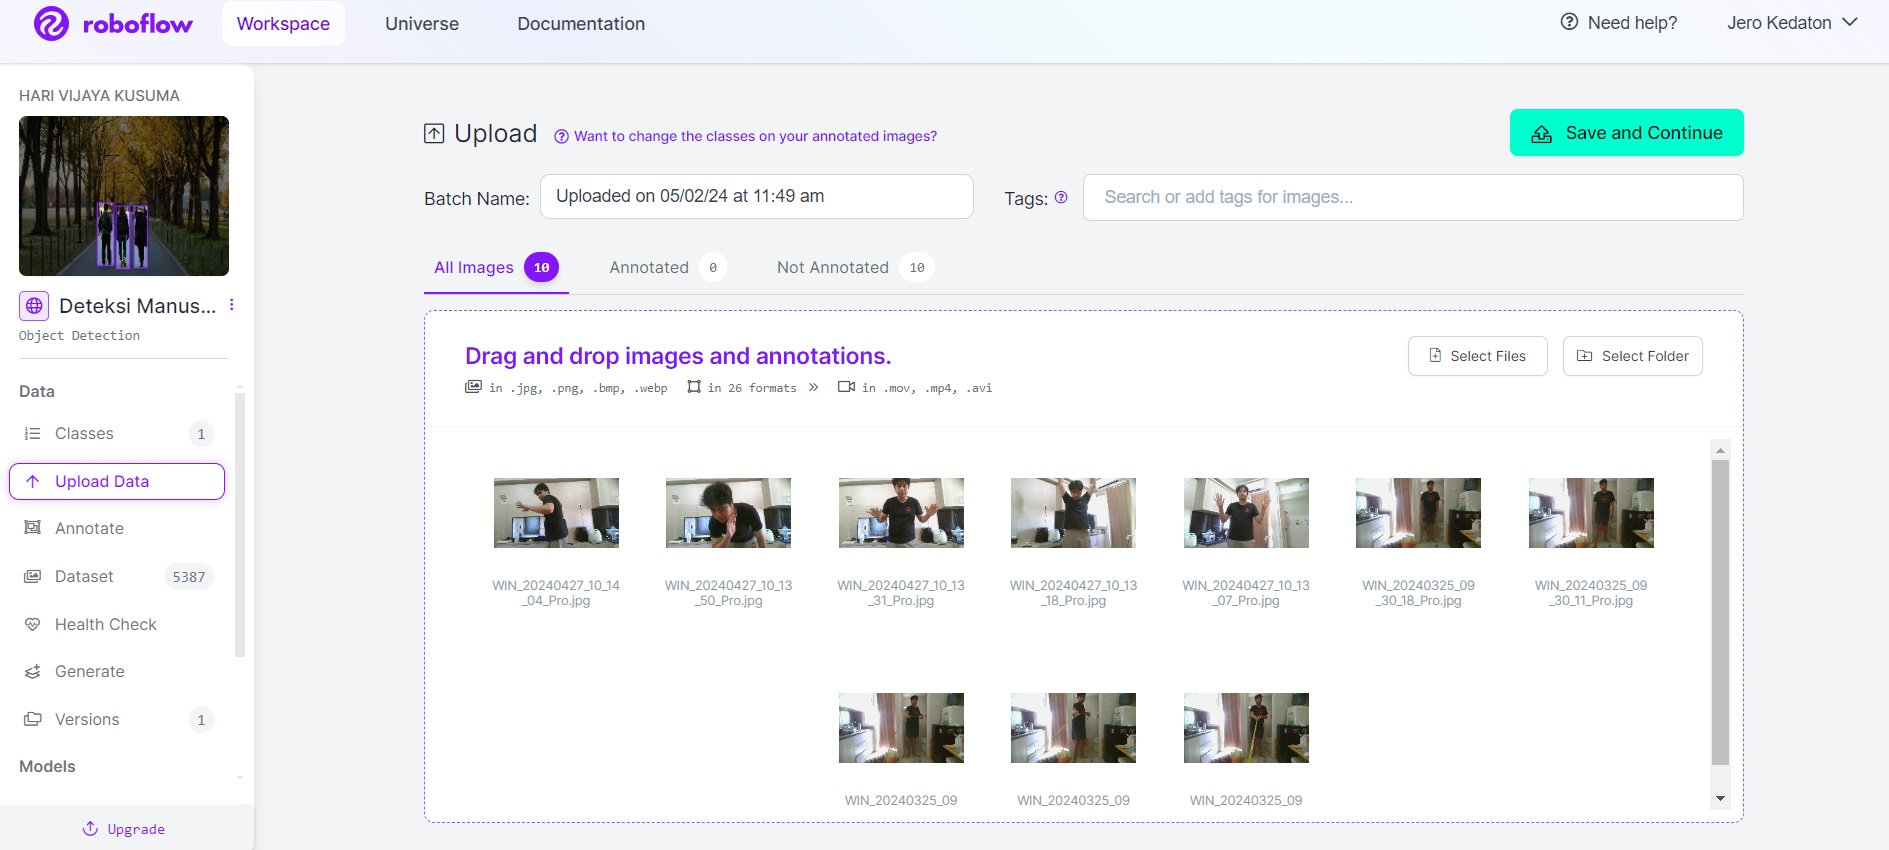
\includegraphics[scale=0.3]{gambar/roboflow upload.jpg}
  % Ubah dengan keterangan gambar yang diinginkan
  \caption{Contoh upload dataset ke roboflow.}
  \label{fig:Mengupload dataset ke roboflow}
\end{figure}

Dataset yang diupload haruslah mencakup beberapa skenario dan mencakup berbagai ukuran Setelah itu melakukan Praproses dataset dengan anotasi, yaitu mengubah ukuran Gambar, menormalkan nilai piksel, dan membaginya menjadi set training, validasi, dan test. Lalu menambah data dengan teknik seperti rotasi, penskalaan, atau membalik untuk meningkatkan keragaman sampel pelatihan.
\begin{figure}[H]
  \centering
  % Ubah dengan nama file gambar dan ukuran yang akan digunakan
  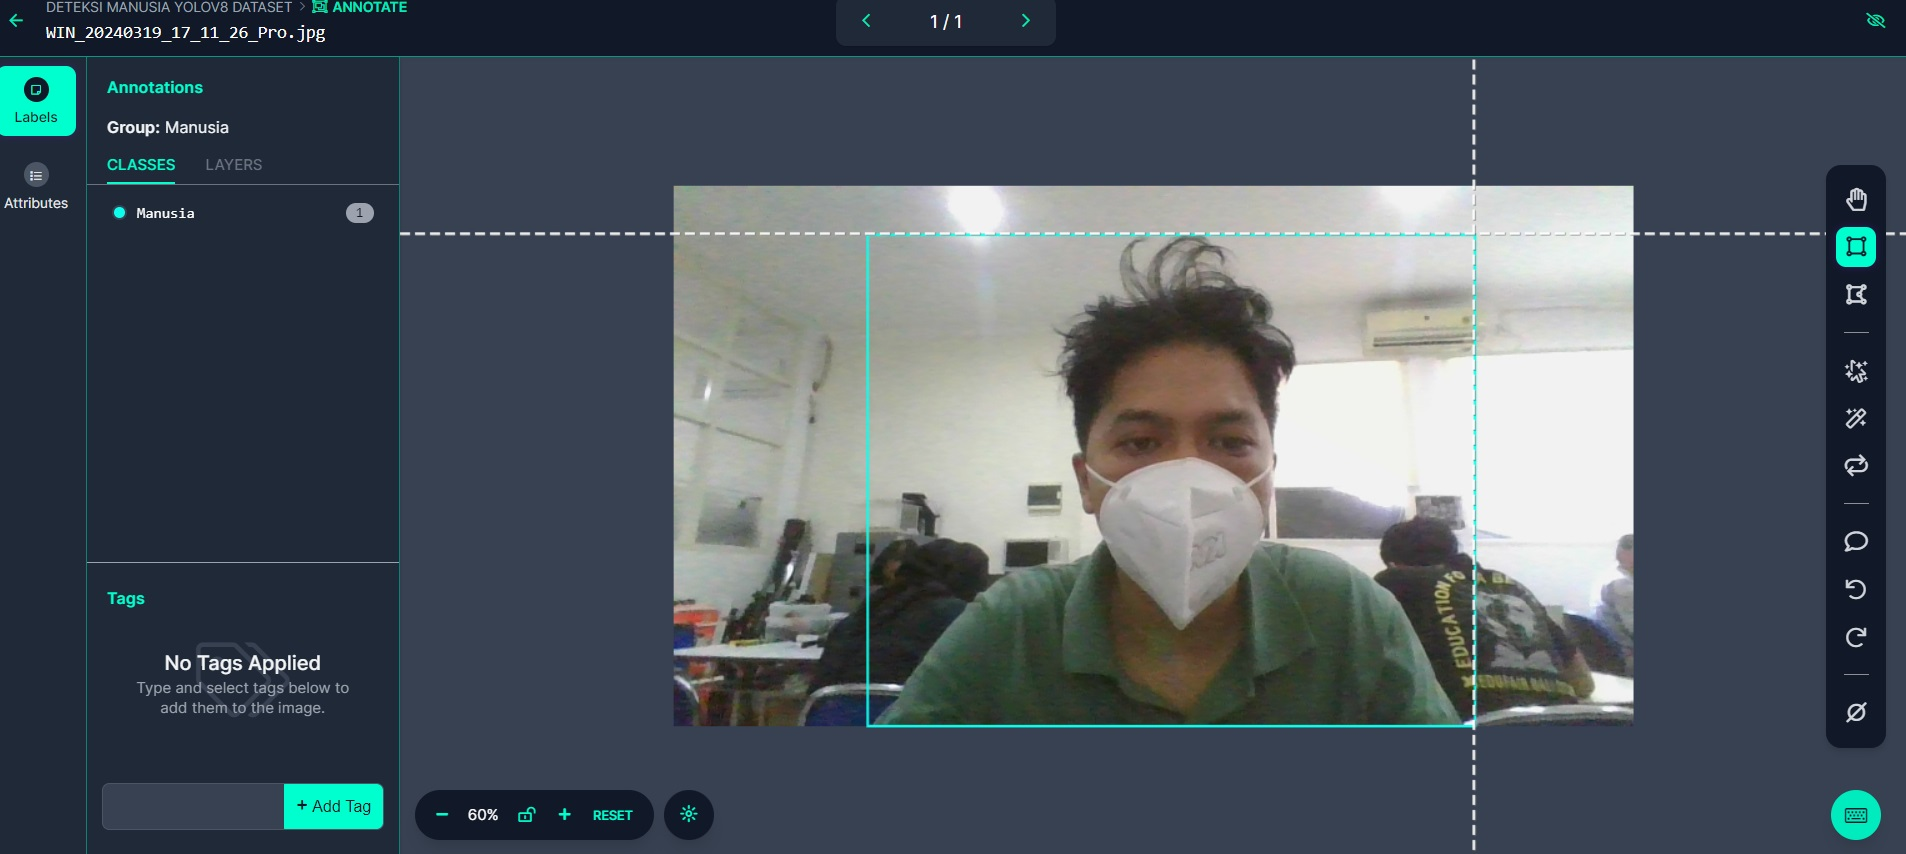
\includegraphics[scale=0.3]{gambar/roboflow anotasi.jpg}
  % Ubah dengan keterangan gambar yang diinginkan
  \caption{Contoh anotasi dataset ke roboflow.}
  \label{fig:Mengupload dataset ke roboflow}
\end{figure}

Dalam proses anotasi penamaan class yang digunakan haruslah sesuai dengan objek yang akan dideteksi. Dalam konteks tugas akhir kali ini obstacle yang dimaksud adalah manusia, maka penamaan class adalah manusia. Selain itu dalam proses anotasi harus diperhatikan posisi objek yang akan dianotasi harus jelas agar tidak ada kesalahan model dalam mendeteksi.

\begin{figure}[H]
  \centering
  % Ubah dengan nama file gambar dan ukuran yang akan digunakan
  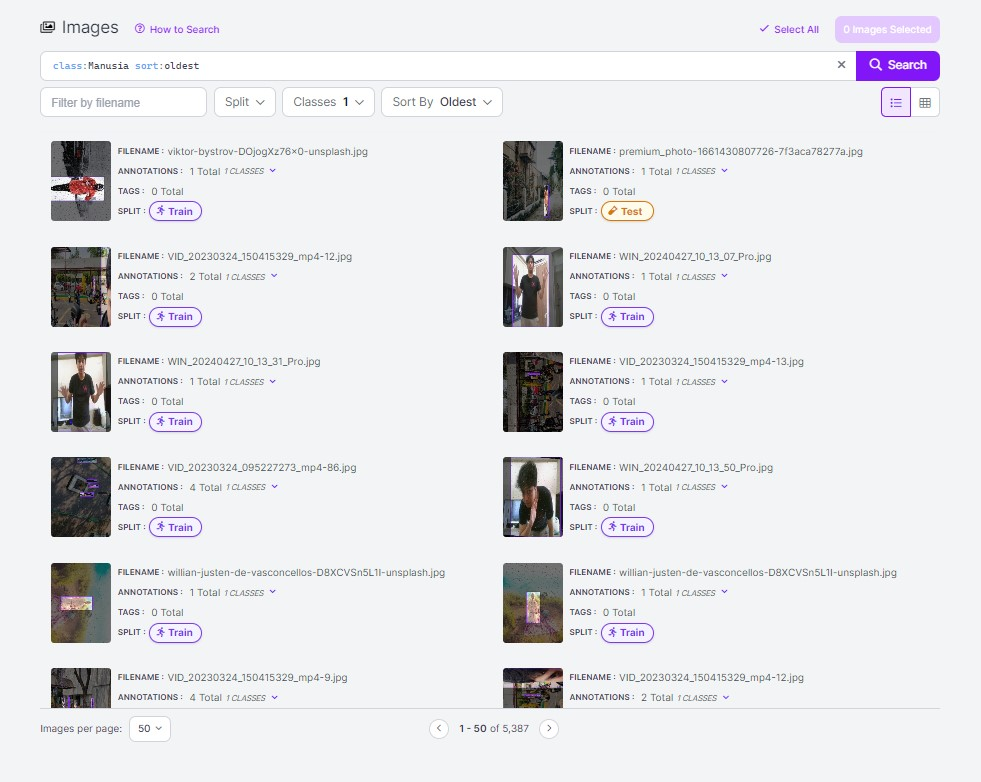
\includegraphics[scale=0.4]{gambar/roboflow Dataset.jpg}
  % Ubah dengan keterangan gambar yang diinginkan
  \caption{Contoh Dataset.}
  \label{fig:Mengupload dataset ke roboflow}
\end{figure}

Setelah seluruh Gambar yang dipilih telah dianotasi, terdapat opsi membuat datasets dan Pemilihan Gambar yang dikelompokkan dari grup batch dataset tesebut diunggah. Pengguna dapat melakukan kombinasi dan Pemilihan secara mendetil tentang Gambar spesifik apa yang dibutuhkan dalam proses pembuatan model sehingga bisa merepresentasikan hasil deteksi objek yang hendak dilakukan. Jika Gambar yang telah
dianotasi telah memenuhi kriteria yang ditetapkan, maka dibuatlah versi baru dataset dengan menekan tombol create new version berwarna biru. Kemudian pengguna dapat memilih Gambar dan mengatur konfigurasi split pada dataset, praproses dataset, serta augmentasi dataset. Berikut tampilan dari Datasets yang siap untuk dibuat yang diGambarkan pada Gambar Diatas.

Selain itu juga terdapat pula fitur preprocesssing datasets yang berasal dari roboflow dimana berguna untuk menstandarkan format Gambar (misalnya, semua Gambar berukuran sama). Langkah ini penting untuk memastikan kumpulan data Anda konsisten sebelum melatih model. Berikut fitur tesebut.

\begin{itemize}
    \item Auto - Orient
    \item Rezise
    \item Grayscale
    \item Auto Adjust Contrast
    \item Isolate Objects
    \item Static Crop
    \item Tile
    \item Modify Classes
    \item Filter Null
\end{itemize}

Adapula fitur Augmentasi data yaitu langkah di mana augmentasi diterapkan pada Gambar yang ada di kumpulan data Anda. Proses ini dapat membantu meningkatkan kemampuan model untuk menggeneralisasi sehingga bekerja lebih efektif pada Gambar yang tidak terlihat. Pada awal proses training tidak digunakan proses augmentasi guna mengevaluasi kualitas datasets yang murni yaitu belum mengalami Augmentasi. Jika augmentasi ditambahkan dan dataset tidak berkinerja sebaik yang diharapkan, maka tidak akan ada dasar untuk membandingkan kinerja model. 

\begin{figure}[H]
  \centering
  % Ubah dengan nama file gambar dan ukuran yang akan digunakan
  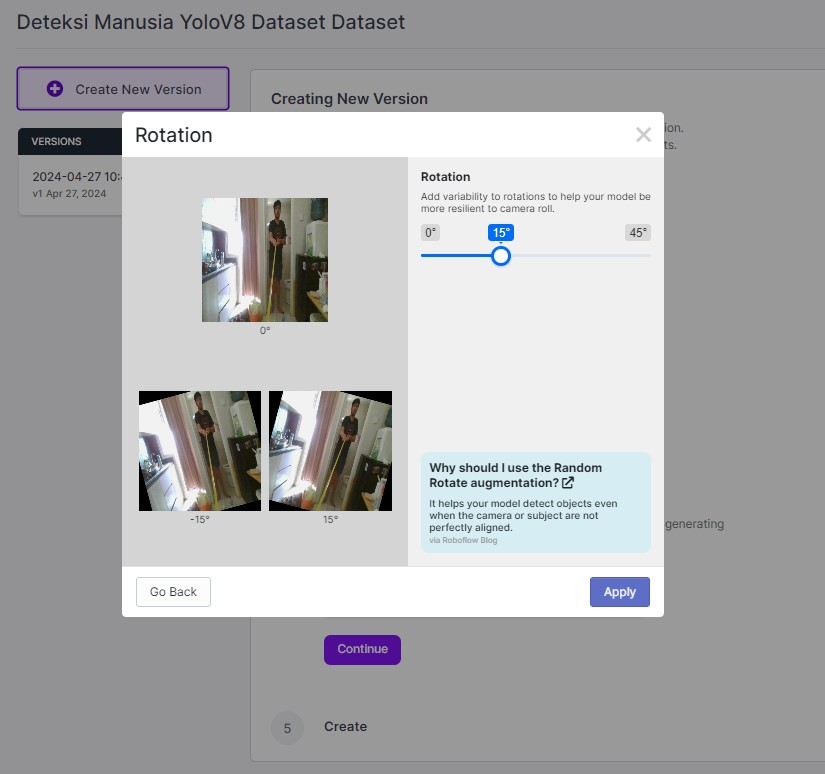
\includegraphics[scale=0.4]{gambar/roboflow augmentasi.jpg}
  % Ubah dengan keterangan gambar yang diinginkan
  \caption{Contoh Augmentasi Dataset.}
  \label{fig:Mengaugmentasi dataset ke roboflow}
\end{figure}

Jika performa model tidak baik tanpa augmentasi, hal yang perlu dilakukan yaitu menyelidiki keseimbangan kelas, representasi data, dan ukuran kumpulan data. Jika terdapat kumpulan data yang modelnya telah berhasil dilatih tanpa augmentasi, maka proses penambahan augmentasi untuk lebih membantu meningkatkan performa model dapat dilakukan.

\subsection{Object Detection YoloV8}
Deteksi Objek dilakukan dengan mendeteksi keberadaan Manusia pada citra yang didapatkan, kemudia keberadaan manusia yang terdeteksi pada citra, akan digambar bounding box pada area yang terdeteksi manusia. Dimana Bounding box yang terdeteksi tersebut akan memilki nilai nilai x dan y dalam posisi pixel pada jendela kamera yang selanjutnya dapat diambil berupa tinggi dan lebar pada pixel yang terdeteksi pada jendela web kamera. Dimana nilai nilai tersebut akan menjadi acuan dalam menentukan jarak objek relatif terhadap kamera. 

\begin{figure}[H]
  \centering
  % Ubah dengan nama file gambar dan ukuran yang akan digunakan
  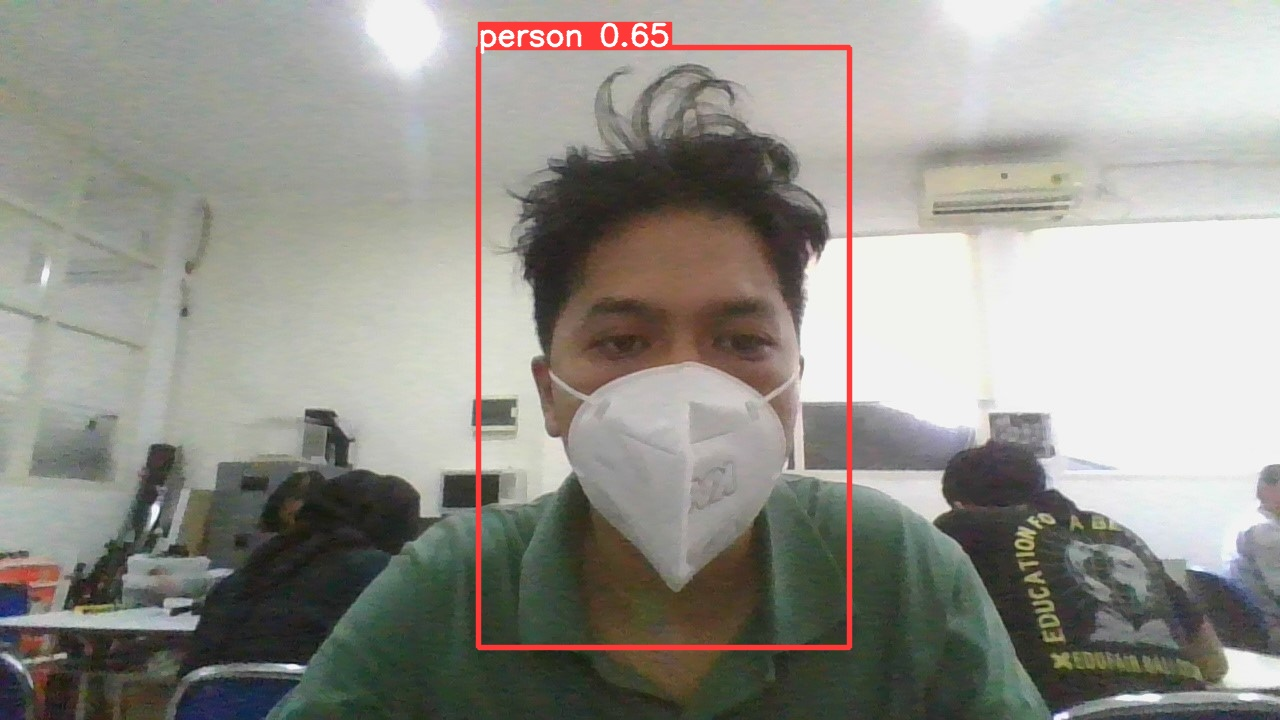
\includegraphics[scale=0.25]{gambar/Foto deteksi untuk bab 2 agung.jpg}
  % Ubah dengan keterangan gambar yang diinginkan
  \caption{Contoh Hasil Deteksi Menggunakan Model YoloV8 yang telah di train.}
  \label{fig:Mengaugmentasi dataset ke roboflow}
\end{figure}


Bounding box yang didapatkan merupakan hasil dari training yang akan dilakukan sehingga model YoloV8 dapat mengidentifikasi kelas yang diinginkan yaitu kelas Manusia. Berikut merupakan contoh gambar hasil dari identifikasi objek yang dihasilkan dari model yang telah dilakukan training. Dapat dilihat hasil deteksi menghasilkan nilai, yang merupakan nilai confidence dari model dimana nilai ini menunjukan seberapa yakin citra yang diinput merupakan bagian class yang terdeteksi.

Dalam proses training akan didapatkan beberapa nilai yang akan menjadi acuan dalam seberapa baik model dalam mendeteksi objek yang terdapat dari input citra, dimana nilai nilai tersebut akan divisualisasikan melalui confusion matrix maupun grafik yang mengindikasikan performa model dalam mendeteksi. berikut contoh gambar confusion matrix

\begin{figure}[H]
  \centering
  % Ubah dengan nama file gambar dan ukuran yang akan digunakan
  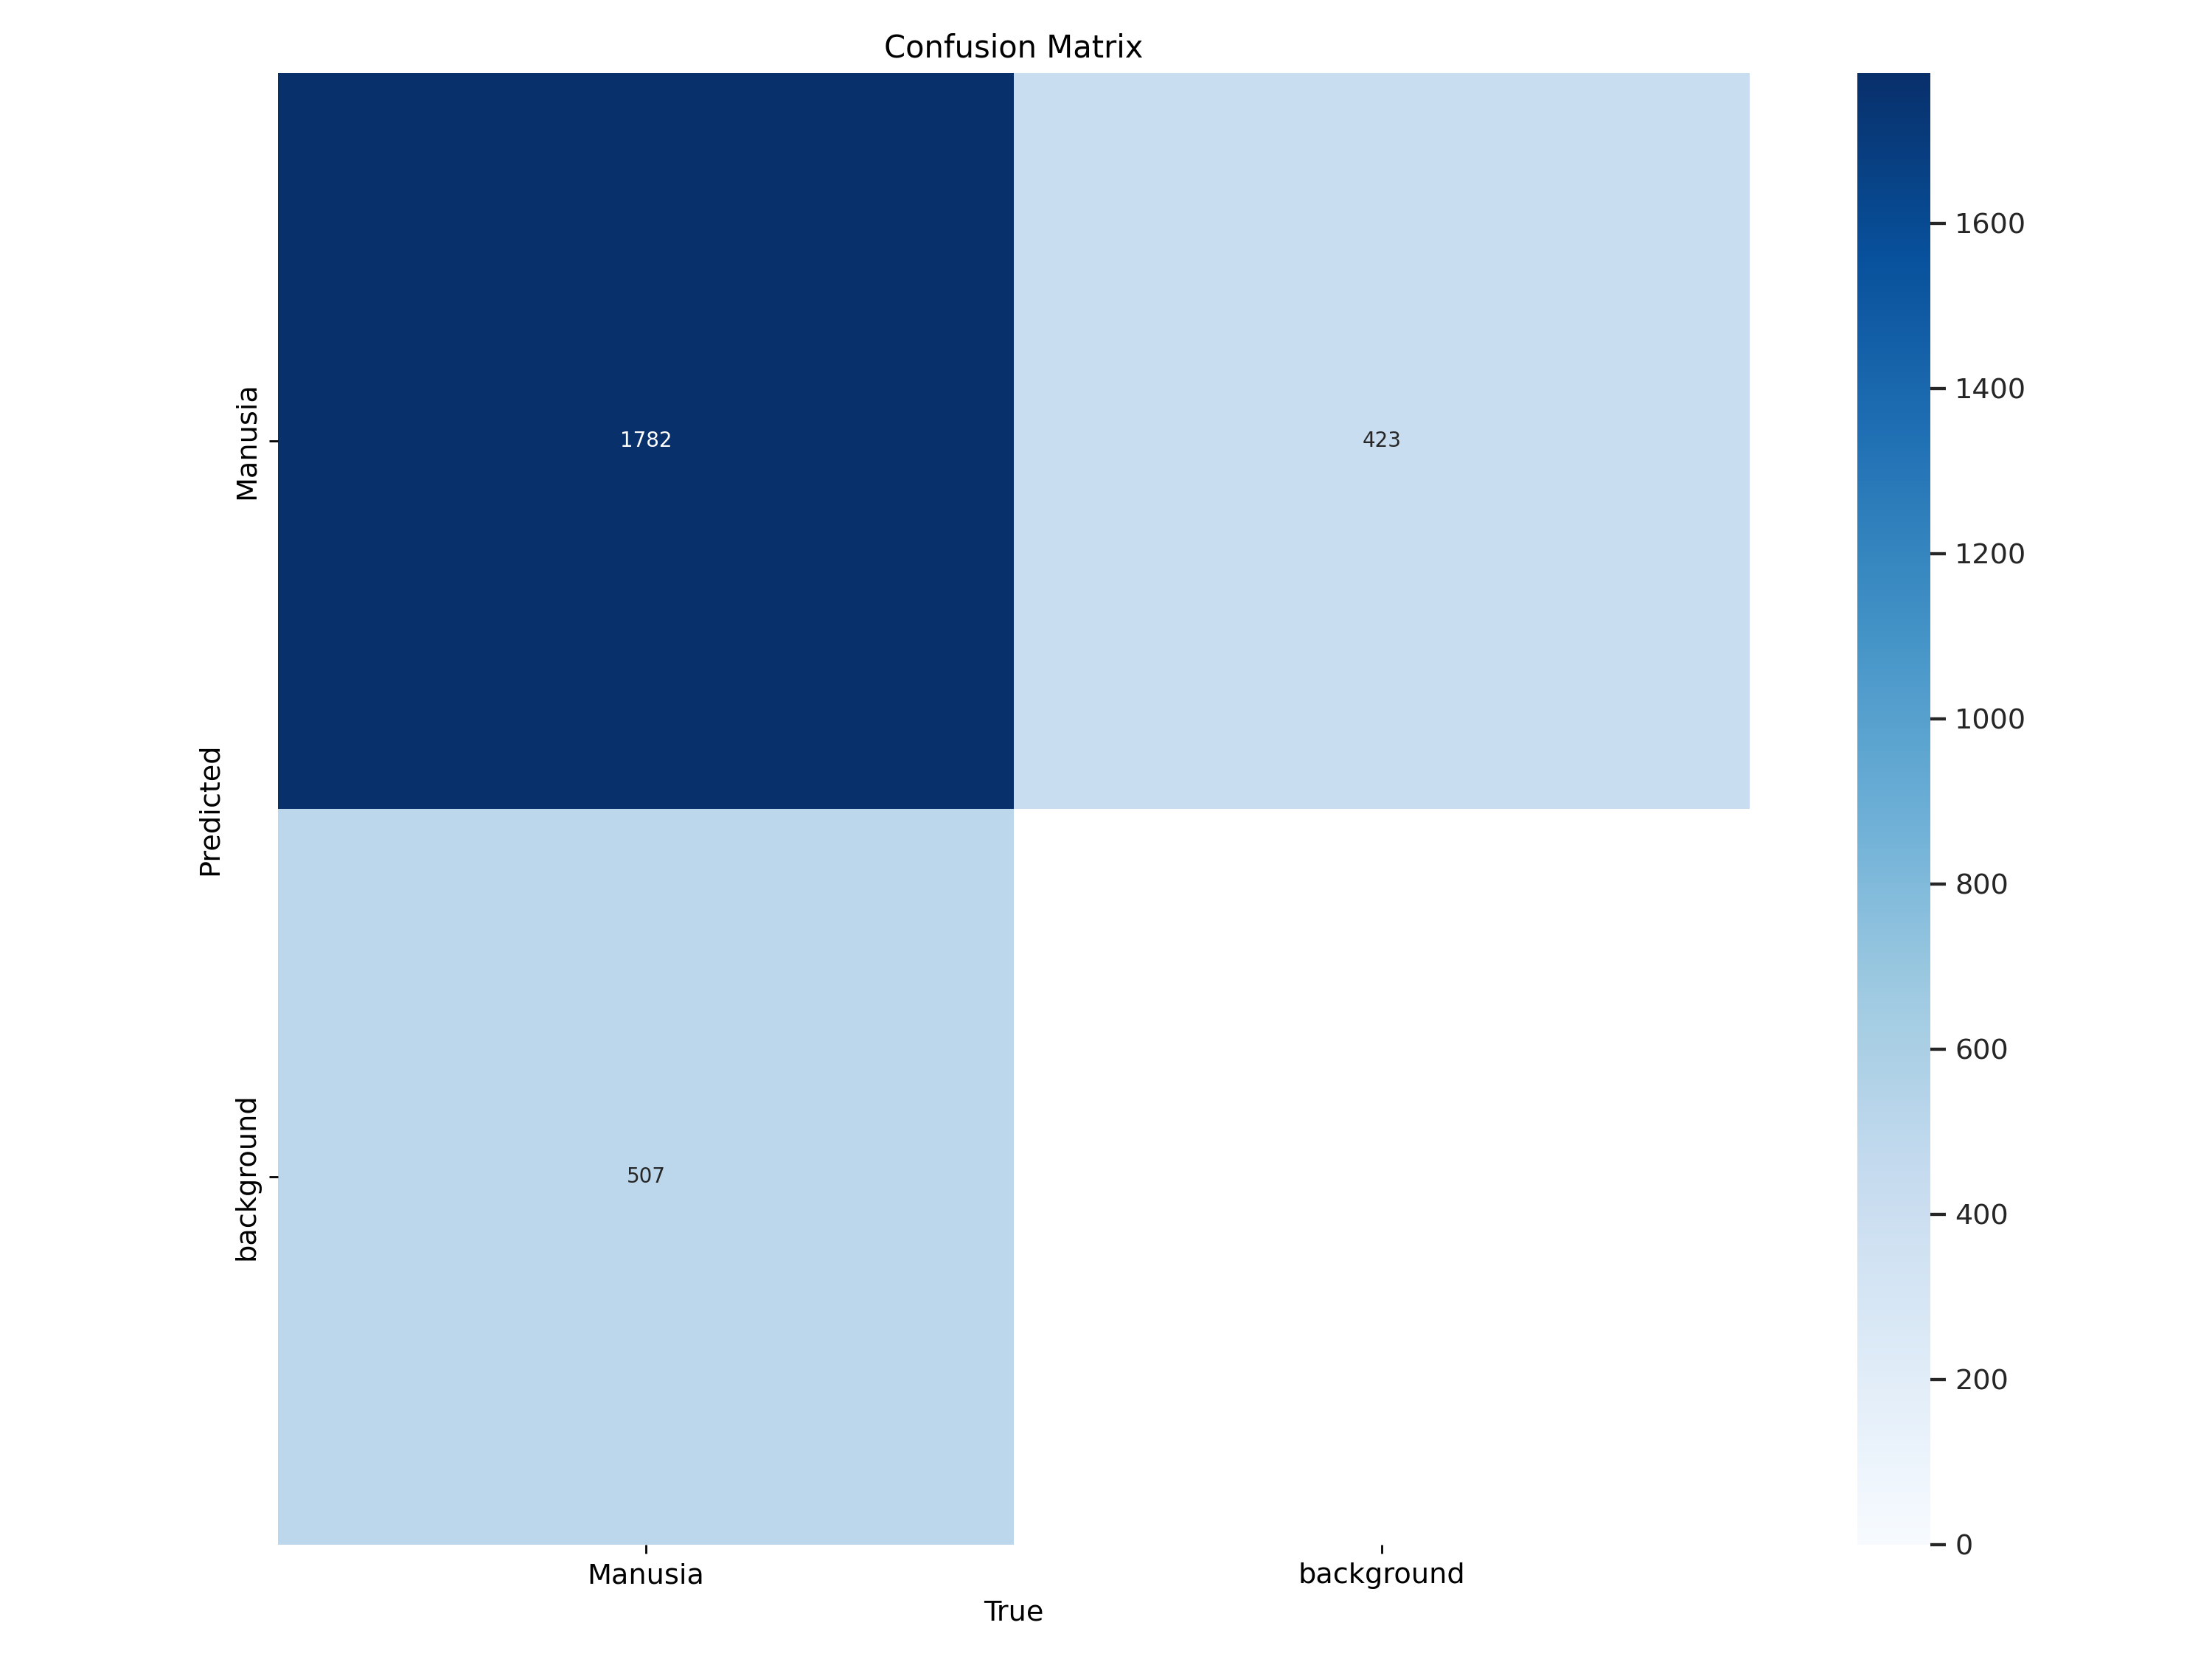
\includegraphics[scale=0.25]{gambar/download.png}
  % Ubah dengan keterangan gambar yang diinginkan
  \caption{Contoh Confusion Matrix model.}
  \label{fig:confusion matrix model}
\end{figure}

Dimana dapat dilihat pada confusion matrix dimana nilai hasil pojok kiri atas merupakan nilai true positive, sedangkan nilai pojok kanan atas merupakan false negatif, nilai pojok kiri bawah adalah false positive, dan terakhir nilai pojok kanan bawah merupakan true negative.

Selain confusion matrix juga terdapat clasification loss. Classification Loss mengukur nilai loss model dalam memprediksi klasifikasi objek yang telah ditentukan melalui proses pelabelan atau anotasi data. Sebuah nilai loss klasifikasi yang rendah menunjukkan bahwa model cenderung menjadi lebih optimal. Localization Loss, pada sisi lain, mencerminkan kinerja sistem dalam menentukan posisi suatu objek. Semakin rendah nilai loss lokalisisasi, semakin baik model yang dihasilkan. Contoh grafik tersebut dapat dilihat pada gambar berikut.

\begin{figure}[H]
  \centering
  % Ubah dengan nama file gambar dan ukuran yang akan digunakan
  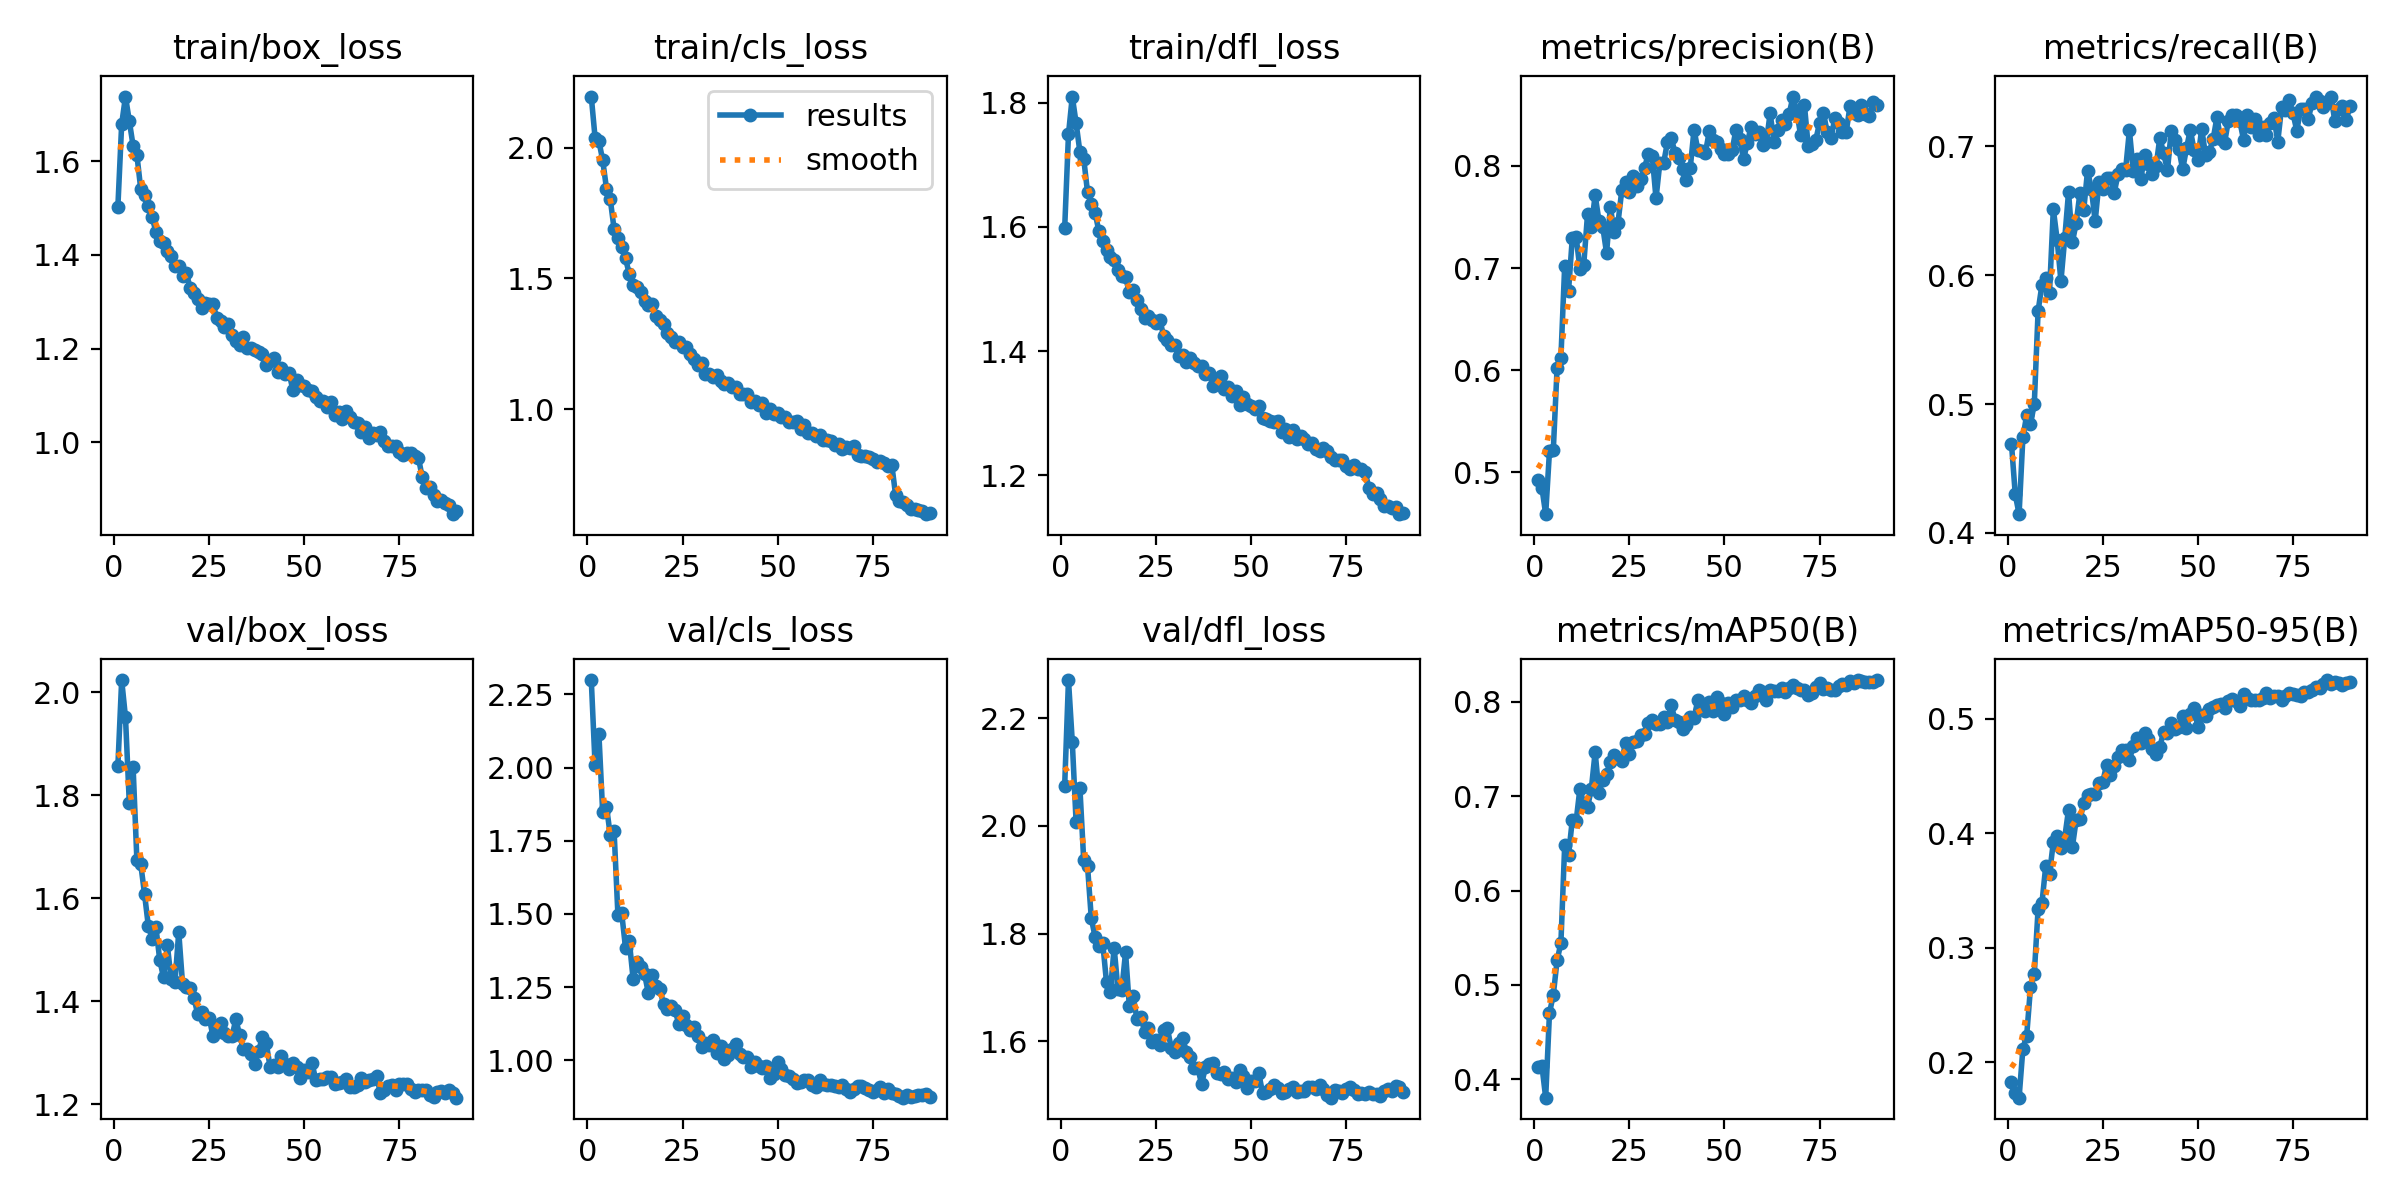
\includegraphics[scale=0.35]{gambar/map dan loss contoh.png}
  % Ubah dengan keterangan gambar yang diinginkan
  \caption{Contoh grafik loss dan mAP model.}
  \label{fig:confusion matrix model}
\end{figure}

Penurunan nilai Localization loss mencerminkan bahwa model yang telah dilatih secara pra-terlatih mampu mengidentifikasi objek dalam Gambar dan menghasilkan koordinat bounding box yang mendekati koordinat bounding box yang diannotasikan. Regularization Loss merujuk pada serangkaian teknik yang bertujuan untuk mengurangi kompleksitas model jaringan saraf selama proses pelatihan, sehingga mencegah terjadinya overfitting. Penerapan berbagai teknik regularisasi dapat membantu mengatasi masalah overfitting dalam jaringan saraf, yang pada gilirannya meningkatkan akurasi model Deep Learning saat dihadapkan pada data baru dari domain permasalahan yang sama. 

Nilai loss regularisasi mencerminkan tingkat kompleksitas model, dengan nilai yang lebih kecil mengindikasikan bahwa model memiliki kemungkinan lebih rendah untuk mengalami overfitting. Loss total mencakup seluruh proses pelatihan model dan dihitung berdasarkan tiga parameter utama, yaitu loss klasifikasi, loss lokalisisasi, dan loss regularisasi, memberikan pandangan menyeluruh terhadap proses pelatihan model. Oleh karena itu, evaluasi kinerja deteksi objek tidak hanya memperhatikan kemampuan model dalam mengklasifikasikan objek, tetapi juga dalam menentukan posisinya dengan akurasi tinggi dan menghindari overfitting yang berlebihan

Dalam penelitian ini, diperkenalkan tiga komponen utama dalam evaluasi kinerja model deteksi objek, yaitu classification loss, localization loss, dan regularization loss. Classification loss mengukur kesalahan model dalam memprediksi klasifikasi objek yang telah diidentifikasi
melalui proses pelabelan atau anotasi data. Semakin rendah nilai classification loss, semakin optimal model dianggap. Di sisi lain, localization loss mengindikasikan kemampuan sistem dalam menentukan posisi objek dalam Gambar. Penurunan nilai localization loss mencerminkan peningkatan kinerja model, terutama dalam menghasilkan koordinat bounding box yang mendekati anotasi yang sebenarnya. Regularisasi, sebagai serangkaian teknik, digunakan untuk mengurangi kompleksitas model jaringan saraf selama pelatihan, dengan tujuan menghindari overfitting. Penerapan berbagai teknik regularisasi membantu meningkatkan generalisasi model terhadap data baru. Nilai regularization loss memberikan Gambaran tentang seberapa kompleks model tersebut, dan nilai yang lebih rendah menunjukkan kemungkinan lebih kecil terjadinya overfitting.

Dapat dilihat pada bagian kanan terdapat grafik precision, dimana grafik ini menunjukkan presisi model, yaitu proporsi prediksi positif yang benar-benar positif. Grafik yang menunjukkan peningkatan secara bertahap menunjukkan bahwa model semakin jarang membuat prediksi positif yang salah. peningkatan ini juga dialami oleh grafik recall yang mana grafik Recall ini mengukur proporsi positif aktual yang berhasil dideteksi oleh model. Grafik dengan peningkatan menunjukkan bahwa model menjadi lebih baik dalam mendeteksi semua kasus positif yang ada. Selanjutnya terdapat grafik mAP (\emph{mean Average Precision}) pada threshold IoU (Intersection over Union) 50\% adalah metrik yang menilai secara keseluruhan kinerja model dalam mendeteksi objek dengan keakuratan yang diberikan. Nilai yang lebih tinggi menunjukkan performa yang lebih baik. dan terakhir mAP50-95 Grafik ini mirip dengan mAP50 tetapi dihitung sebagai rata-rata dari IoU yang berkisar dari 50\% hingga 95\%. Ini adalah metrik yang lebih ketat dan menunjukkan kinerja model secara lebih rinci dalam berbagai tingkat ketat deteksi.

\subsection{Estimasi Pose MediaPipe}
Deteksi pose dilakukan dengan menggunakan Python dengan library OpenCV dan frame-work MediaPipe menggunakan fungsi pose detection saat objek manusia terdeteksi dalam frame citra . Framework MediaPipe digunakan untuk mendapatkan landmark pada tubuh peraga, lalu landmark yang relevan akan digambarkan garis berbentuk kerangka yang sesuai dengan pose tubuh peraga. Dalam penelitian ini, landmark yang relevan yaitu keypoint siku atas hingga lengan bawah dan bahu kanan dan kiri. Titik keypoint yang digunakan pada estimasi pose dapat dilihat pada Tabel dibawah ini.

\begin{longtable}{|c|c|}
  \caption{Tabel Keypoint yang digunakan}
  \label{tb:EnergiKecepatan}                                   \\
  \hline
  \rowcolor[HTML]{C0C0C0}
  \textbf{Nomor Keypoint} & \textbf{Nama Keypoint}  \\
  \hline
  11            & RIGHT\_SHOULDER        \\
  12            & LEFT\_SHOULDER         \\
  14            & RIGHT\_ELBOW           \\
  16            & RIGHT\_WRIST           \\
  \hline
\end{longtable}

Dari titik landmark yang didapat akan diambil jarak terhadap pixelnya dimana nilai pixel yang didapatkan akan menjadi acuan dalam perhitungan yang akan digunakan untuk menghindari obstacle. berikut contoh landmark pada data citra.

\begin{figure}[H]
  \centering
  % Ubah dengan nama file gambar dan ukuran yang akan digunakan
  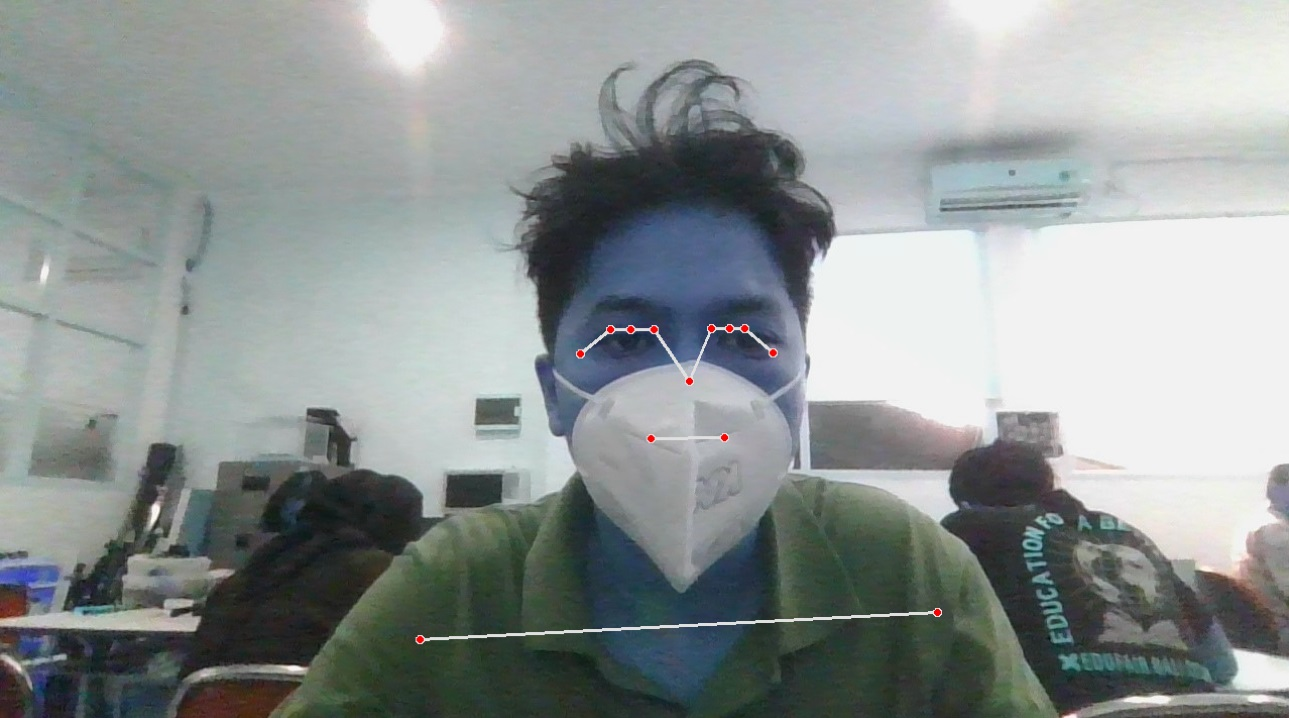
\includegraphics[scale=0.35]{gambar/fotomediapipe.jpg}
  % Ubah dengan keterangan gambar yang diinginkan
  \caption{Contoh hasil deteksi pose.}
  \label{fig:confusion matrix model}
\end{figure}

\begin{figure}[H]
  \centering
  % Ubah dengan nama file gambar dan ukuran yang akan digunakan
  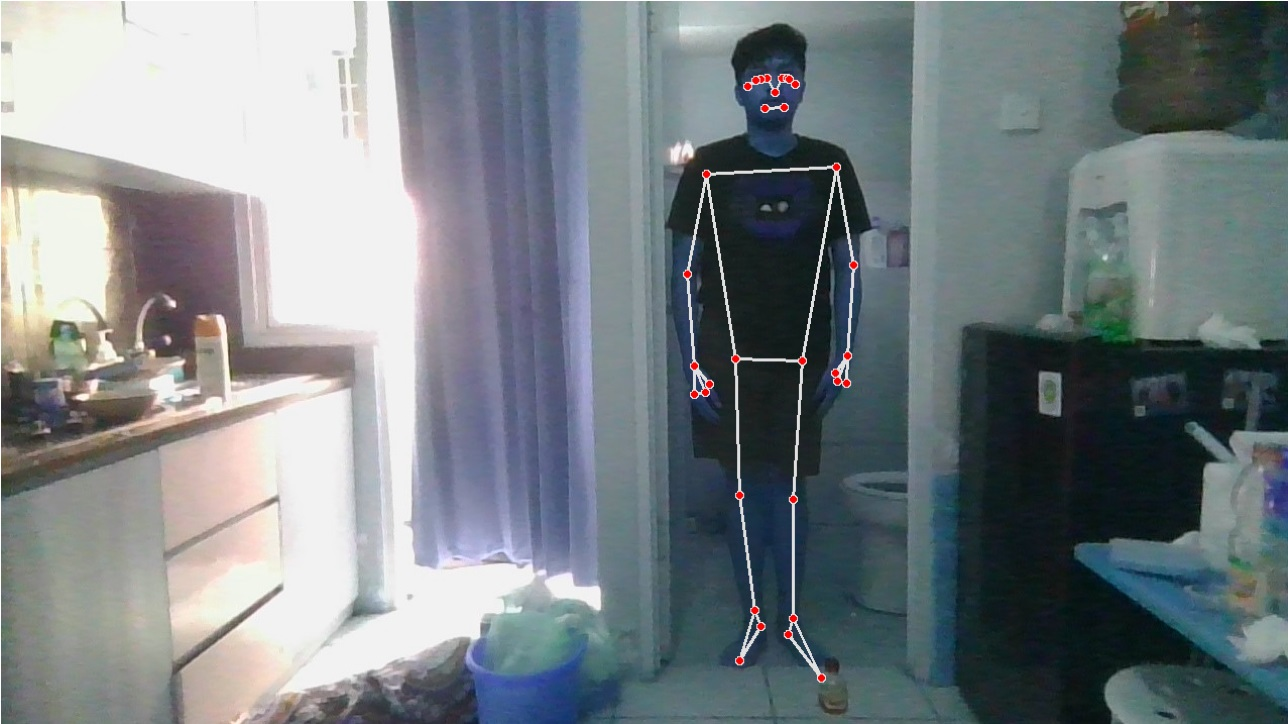
\includegraphics[scale=0.35]{gambar/fotomediapipe2.jpg}
  % Ubah dengan keterangan gambar yang diinginkan
  \caption{Contoh hasil deteksi pose seluruh tubuh.}
  \label{fig:confusion matrix model}
\end{figure}

Pengunaan landmark lengan dan bahu sebagai acuan dalam perhitungan berdasar pada visibilitas, dimana visibilitas kedua landmark ini cenderung lebih baik ketimbang landmark kaki dan kepala terutama dalam kasus penghindaran manusia. Dimana dalam jarak dekat kedua landmark ini akan lebih terlihat ketimbang landmark lainnya. Selain itu penggunaan landmark ini juga dapat menghasilkan nilai yang lebih konsisten ketimbang landmark lainnya.

\subsection{Perhitungan Rumus}

Untuk dapat menentukan jarak, pertama tama model Yolo akan digunakan untuk mendeteksi class Manusia yang akan menjadi obstacle dalam tugas akhir ini. Dari hasil deteksi yang didapat akan digambar Bounding Box penanda kelas telah terdeteksi. Dimana dalam bounding box tersebut juga akan digambar Estimasi Pose dari MediaPipe. Kedua hasil deteksi ini yaitu Bounding Box dan Pose yang dihasilkan akan digunakan untuk mendapat estimasi jarak berdasarkan rumus yang akan dijabarkan, dimana hasil dari jarak yang didapatkan akan dipetakan perpindahannya dalam grid. Dimana grid ini akan menjadi acuan dari keputusan belok yang akan diambil. berikut merupakan contoh gambar pemetaan hasil deteksi dan pengambilan keputusan belok.

\begin{figure}[H]
  \centering
  % Ubah dengan nama file gambar dan ukuran yang akan digunakan
  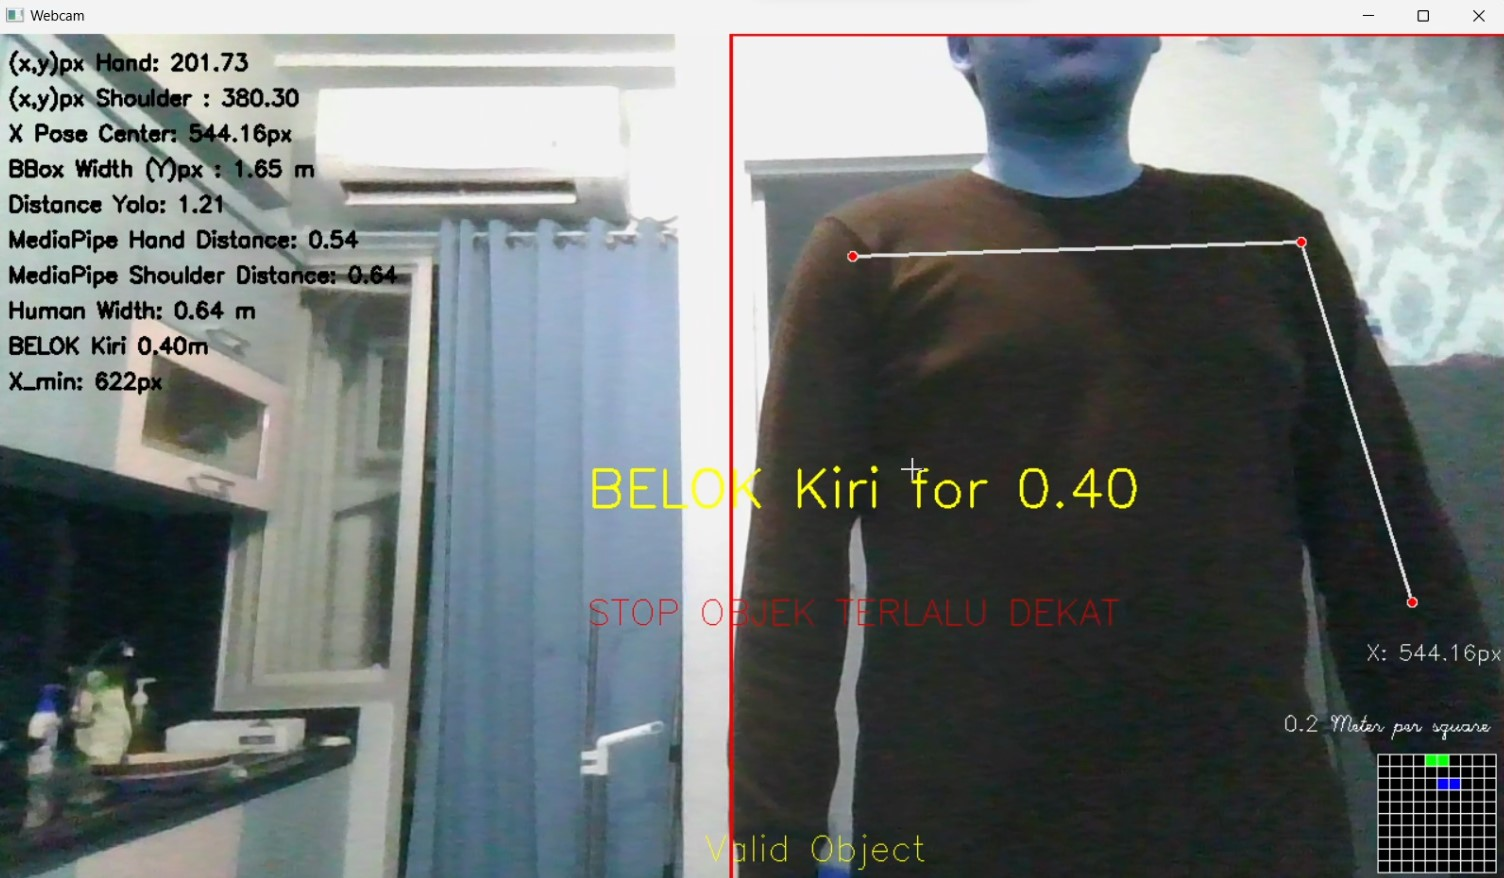
\includegraphics[scale=0.35]{gambar/belokkiri.jpg}
  % Ubah dengan keterangan gambar yang diinginkan
  \caption{Contoh Penerapan hasil perhitungan jarak dan pemetaan grid.}
  \label{fig:Penerapan hasil perhitungan jarak dan pemetaan grid}
\end{figure}

Dapat dilihat bahwa Terdapat banyak variabel pada jendela web kamera. Semua variabel tersebut memiliki peran masing masing, yang akan membantu mendapatkan nilai yang akan dipetakan dalam grid pada bagian kiri bawah.

Dalam Tugas Akhir ini terdapat beberapa variabel yang akan diukur. Variabel-variabel tersebut yaitu jarak manusia, lebar manusia, dan posisi manusia. Dimana Jarak manusia ini akan dibedakan menjadi 2 perhitungan, dimana 2 perhitungan ini berdasarkan 2 hasil deteksi yang didapatkan yaitu bounding box dan pose.

\subsubsection*{1. Perhitungan Jarak Obstacle berdasarkan Bounding Box}
Salah satu cara untuk mendapatkan jarak melalui Bounding Box adalah dengan menggunakan \emph{Focal Length Pixel}. Fokus panjang dalam piksel, atau \emph{focal length pixel}, adalah sebuah konversi dari fokus panjang lensa kamera yang biasanya diukur dalam milimeter ke dalam satuan piksel. Ini adalah konsep kunci dalam fotogrametri dan visi komputer yang digunakan untuk menghubungkan informasi visual yang diperoleh dari kamera ke ukuran fisik dalam dunia nyata.

Dalam konteks tugas akhir ini Fokus panjang dalam piksel digunakan untuk mengkonversi ukuran halangan dari unit piksel menjadi unit meter. Ini penting karena kursi roda otonom perlu memahami jarak nyata ke halangan untuk mengambil keputusan navigasi yang tepat. Dalam penggunaannya dapat dilihat dalam rumus berikut.

\begin{equation}
    focal\_length\_pixel = \left (\frac{jarak\times tinggi\_bounding\_box }{tinggi\_objek\_nyata}\right )
\end{equation}

Fokus panjang dalam piksel adalah parameter penting dalam perhitungan jarak Anda. Ini digunakan untuk mengonversi pengukuran dari ruang gambar (piksel) menjadi dimensi dunia nyata (seperti meter). Nilai ini mewakili fokus panjang lensa kamera dalam satuan piksel, yang diperoleh dari prosedur kalibrasi. 

Saat menghitung jarak ke objek dengan menggunakan tinggi dari bounding box yang terdeteksi oleh YOLO, dikombinasikan dengan tinggi nyata objek yang diketahui dan fokus panjang dalam piksel. penerapannya dapat dilihat sebagai berikut :

\begin{equation}
    jarak = \left ( \frac{focal\_length\_pixel \times tinggi\_objek\_nyata}{tinggi\_bounding\_box} \right )
\end{equation}

Di sini, tinggi\_objek\_nyata mungkin merupakan tinggi rata-rata orang atau objek lain yang diidentifikasi sebagai obstacle. Dengan menggunakan tinggi bounding box yang dideteksi oleh YOLOv8, kursi roda dapat menghitung jarak ke objek tersebut, yang sangat penting untuk menghindari benturan dan pengambilan keputusan.

\subsubsection*{2. Perhitungan Jarak Obstacle berdasarkan Pose}
Salah satu pendekatan yang baik dalam menentukan jarak dengan pose adalah menggunakan metode Jarak Euclidean. Jarak Euclidean dalam piksel adalah metode untuk mengukur jarak lurus antara dua titik dalam ruang gambar, yang biasanya diukur dalam piksel. Dalam konteks tugas akhir ini yang melibatkan kursi roda otonom dengan integrasi MediaPipe, pengukuran ini sangat penting untuk berbagai fungsi, terutama dalam analisis pose dan penilaian proporsi objek dalam citra yang dihasilkan oleh kamera. 

\begin{equation}
    {jarak\_euclidean} = \sqrt{(x_2 - x_1)^2 + (y_2 - y_1)^2} \times scale\_factor
\end{equation}

Rumus ini menghasilkan jarak antara dua titik dalam satuan yang sama dengan satuan koordinat \emph{x1,y1} dan \emph{x2,y2} Biasanya, jika koordinat-kordinat ini diukur dalam piksel, maka jarak yang dihasilkan juga akan dalam piksel.

Penambahan faktor skala ke dalam perhitungan jarak Euclidean berguna ketika perlu mengkonversi jarak dari satu unit ke unit lain, atau ketika koordinat titik disesuaikan ke skala tertentu yang tidak merefleksikan dimensi sebenarnya dalam piksel. Normalisasi Koordinat Dalam banyak aplikasi visi komputer, koordinat titik mungkin dinormalisasi ke skala [0, 1]. Di sini \emph{x1,y1} dan \emph{x2,y2} dalah proporsi dari lebar dan tinggi gambar. Untuk menghitung jarak nyata dalam piksel, perlu mendapatkan hasik kali dari rumus Euclidean dengan dimensi gambar.

Dari perhitungan diatas masih didapatkan jarak yang bernilai pixel. Dalam konteks perhitungan jarak perlu menggunakan niali standar dalam Meter agar perhitungan tersebut sesuai dengan kaidah yang berlaku pada umumnya. Agar nilai pixel tersebut dapat berubah menjadi meter maka perlu dilakukan kalibrasi menggunakan nilai K. nilai K merupakan nilai kalibrasi berdasarkan pengukuran eksperimental. rumusnya dapat dilihat sebagai berikut. 

\begin{equation}
    jarak\_meter = \left(\frac{k}{{jarak\_pixel}}\right)
\end{equation}

Nilai k menentukan seberapa besar pengaruh jarak dalam piksel terhadap jarak dalam meter. Nilai yang lebih besar atau lebih kecil akan secara langsung mempengaruhi hasil perhitungan jarak. Misalnya, nilai k yang lebih besar akan menghasilkan jarak yang lebih kecil untuk jumlah piksel yang sama. Nilai ini digunakan dalam konteks yang sangat spesifik di mana parameter tersebut menggambarkan hubungan langsung antara ukuran piksel dan jarak atau dimensi nyata, berdasarkan asumsi spesifik tentang geometri scene dan karakteristik kamera.

Nilai ini harus dikalibrasi secara akurat agar sesuai dengan karakteristik spesifik kamera dan setup yang digunakan. Kalibrasi yang tidak tepat akan menghasilkan pengukuran jarak yang tidak akurat, yang bisa berdampak pada keputusan navigasi kursi roda otonom. berikut rumus untuk pengkalibrasian nilai K:

\begin{equation}
    k ={{Jarak\_nyata\_objek}\times{Ukuran\_objek\_dalam\_piksel}}
\end{equation}

Nilai k mungkin perlu disesuaikan jika kondisi lingkungan berubah, seperti perubahan pencahayaan yang mempengaruhi visibilitas atau ketepatan deteksi landmark oleh MediaPipe.

\subsubsection{3. Perhitungan Lebar Obstacle Berdasarkan Pose}
Dalam perhitungan lebar juga menggunakan perhitungan jarak euclidean namun yang membedakan adalah konteks spesifikasi aplikasi. Dimana kedua pendekatan ini berbeda dalam aplikasi dan konteksnya. 

\begin{equation}
    {width\_pixel} = \sqrt{(x_2 - x_1)^2 + (y_2 - y_1)^2} \times {scale\_factor}
\end{equation}

Dimana sesuai dengan dijelaskan sebelumnya nilai output yang didapatkan adalah pixel dari lebar manusia. untuk memetakan lebarnya pixel ke meter maka perlulah membuat sebuah rumus konversi yang menentukan ukuran dalam pixel (yang merupakan ukuran digital dan relatif dikonversikan ke ukuran dunia nyata (meter)). sehingga rumusnya menjadi : 
\begin{equation}
    {width\_meters} = width\_pixel \times scale\_factor
\end{equation}

Dengan mengalikan lebar objek dalam piksel dengan faktor skala, hasilnya adalah lebar objek dalam meter. Rumus ini berguna, misalnya, dalam aplikasi dimana perlu untuk mengetahui dimensi fisik objek dalam dunia nyata untuk membuat keputusan atau pengukuran yang tepat.

Faktor skala adalah nilai yang mengonversi ukuran dari unit piksel ke unit meter. Nilai ini diperoleh melalui proses kalibrasi. Faktor skala menentukan berapa meter yang diwakili oleh setiap piksel dalam gambar, berdasarkan jarak kamera ke objek dan pengaturan kamera lainnya seperti fokus panjang. Selain itu perlu diketahui bahwa faktor skala yang digunakan pada rumus ini berbeda dengan rumus jarak yang sebelumnya dijabarkan. berikut rumus untuk mengkalibrasi faktor skala dalam konteks lebar objek:

\begin{equation}
    {scale\_factor} = \frac{{dimensi\_nyata\_rata-rata}}{{ukuran\_dalam\_piksel\_rata-rata}}
\end{equation}

Nilai-nilai ini dapat digunakan dalam kode untuk mengonversi ukuran dalam piksel ke ukuran nyata berdasarkan pengukuran yang telah dikalibrasi. Dan sekali lagi pastikan kalibrasi dilakukan dengan baik dan benar agar mendapatkan hasil yang akurat. 

\subsection{Visualisasi hasil deteksi dalam Grid}
Dalam tugas akhir ini, kursi roda otonom harus dapat mengetahui posisi obstacle yang akan dilaluinya. Oleh karena itu perlu dibuatnya sebuah peta yang dapat digunakan sebagai acuan kursi roda untuk mengambil tindakan berdasarkan jarak obstacle dan lebar obstacle yang akan menjadi acuan untuk menjawab permasalan, yaitu di titik mana kursi roda harus menghindar dan berhasilkah obstacle dihindari. Grid menjadi salah satu pendekatan terbaik dalam memetakan hasil deteksi, dimana penggunaan grid tidak hanya mempermudah dalam pengambilan tindakan, namun grid juga memberikan visualisasi mudah untuk dimengerti. Dimana ukuran grid juga dapat dicustom sesuai dengan kebutuhan, baik dimensi maupun tampilannya. 

Setelah perhitungan rumus diatas diimplementasikan dalam kode. Maka akan didapatkan beberapa variabel penting yang akan digunakan dalam memetakan posisi maupun ukuran obstacle dalam grid. sebelum itu berikut tampilan grid yang digunakan. 

\begin{figure}[H]
  \centering
  % Ubah dengan nama file gambar dan ukuran yang akan digunakan
  
\includegraphics[scale=0.3]{gambar/gridtanpakamera2.jpg}
  % Ubah dengan keterangan gambar yang diinginkan
  \caption{Grid 10x10.}
  \label{fig:Grid10x10}
\end{figure}

Penggunaan grid 10x10 didasari atas hasil citra dan performa model. Dimana baik bounding box maupun pose memiliki keterbatasan dimana hasil perhitungannya tidak melebihi parameter yang akan ditetapkan pada grid. Dimana parameter tersebut ialah sebagai berikut

\begin{figure}[H]
  \centering
  % Ubah dengan nama file gambar dan ukuran yang akan digunakan
  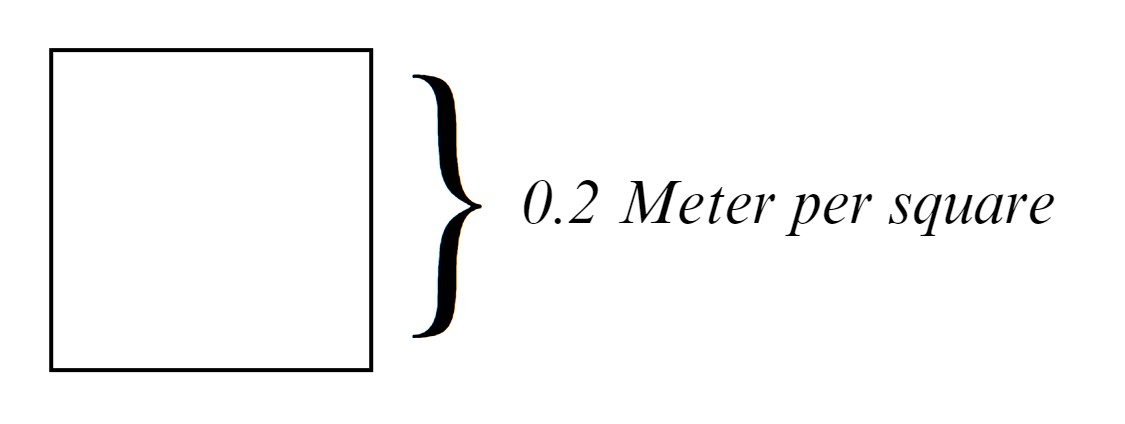
\includegraphics[scale=0.35]{gambar/02meter.jpg}
  % Ubah dengan keterangan gambar yang diinginkan
  \caption{Parameter untuk setiap kotak grid.}
  \label{fig:Parameter grid}
\end{figure}

Dapat dilihat dari gambar diatas, merupakan tetapan yang didasari dari performa diatas yang dimana setiap kotak dalam grid tersebut akan bernilai 0.2 meter baik dalam posisi vertikal maupun horizontal.

Agar dapat memetakan objek dengan baik dalam grid maka diperlukannya index untuk mengetahui posisi relatif kiri dan kanan objek terhadap kamera. Dimana untuk 10 kotak horizontal akan dibagi dimana Index 1 sampai 5 akan dikategorikan sebagai index kiri, dan index 6 hingga 10 akan dikategorikan dalam index kanan. pengambilan keputusan ini terkait dengan posisi kursi roda statis pada grid yang akan digambarkan sebagai berikut

\begin{figure}[H]
  \centering
  % Ubah dengan nama file gambar dan ukuran yang akan digunakan
  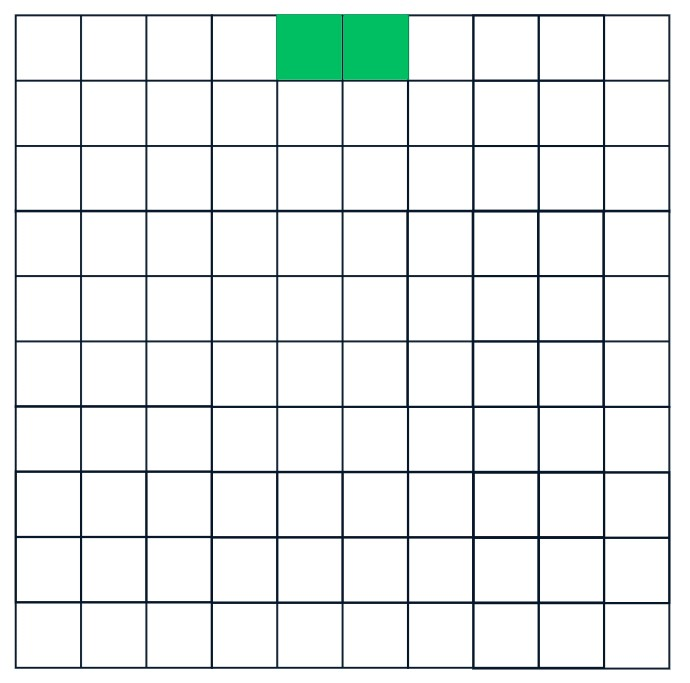
\includegraphics[scale=0.35]{gambar/gridkamera.jpg}
  % Ubah dengan keterangan gambar yang diinginkan
  \caption{Posisi Kursi Pada grid.}
  \label{fig:Posisi}
\end{figure}

Dapat dilihat posisi kursi roda mengambil 2 kotak grid hijau pada bagian (5,1) dan (6,1) dimana keputusan ini didasarkan lebar kursi roda yang sesuai dengan ukuran grid ada. Pemilihan posisi atas menentukan index mana yang merupakan bagian kiri maupun kanan dalam grid. Dengan posisi atas ditetapkan sebagai posisi konstan kursi roda dan hasil input citra yang didapatkan bersebrangan dengan hasil deteksi (mirror) maka index dapat diposisikan sebagai berikut:

\begin{figure}[H]
  \centering
  % Ubah dengan nama file gambar dan ukuran yang akan digunakan
  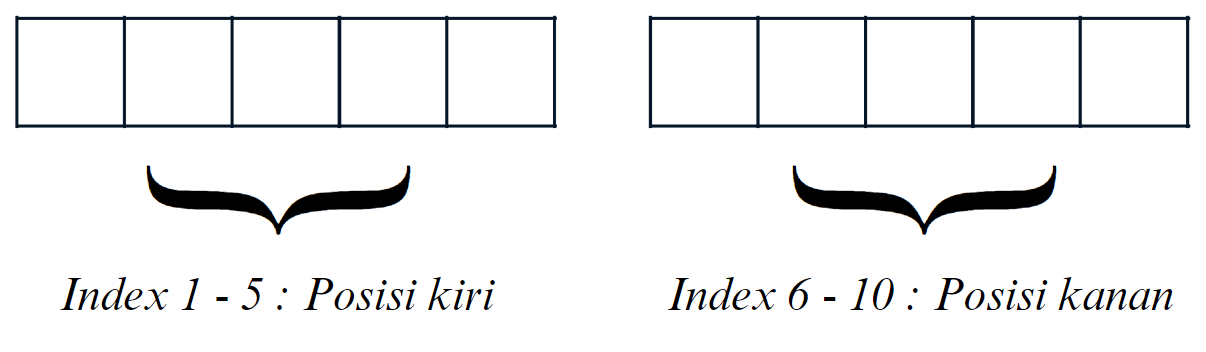
\includegraphics[scale=0.3]{gambar/posisi index sebenarnya.png}
  % Ubah dengan keterangan gambar yang diinginkan
  \caption{Kategori Posisi berdasarkan Index.}
  \label{fig:Kategori Posisi berdasarkan index.}
\end{figure}

Pengkategorian ini berperan penting dalam pengambilan keputusan belok kursi roda dimana nantinya hasil deteksi yang berupa jarak , lebar serta posisi relatif akan ditampilkan pada grid.

Secara horizontal posisi objek hasil deteksi akan diambil berdasarkan Nilai perpindahan titik X bounding box bawah relatif terhadap pixel. Yang mana nilainya akan disesuaikan dengan Resolusi frame yang didapatkan oleh kamera. Dimana akan dibuat patokan untuk posisi tertentu yang melambangkan perpindahan sebesar 0.2 meter secara horizontal.  Dengan asumsi bahwa kursi roda bergerak dan objek diam. maka hanya posisi objek yang terdeteksi didepanlah yang akan menjadi patokan penghindaran. Apabila objek terdeteksi namun saat berjalan maju objek menghilang maka kursi roda tidak perlu melakukan penghindaran. Oleh karena itu ditetapkan parameter jarak pada objek yang terdeteksi berdasarkan vertikal. Namun sebelum membahas lebih lanjut, akan dijelaskan secara rinci mengenai pemetaan hasil deteksi melalui hasil variabel yang didapat.

\begin{figure}[H]
  \centering
  % Ubah dengan nama file gambar dan ukuran yang akan digunakan
  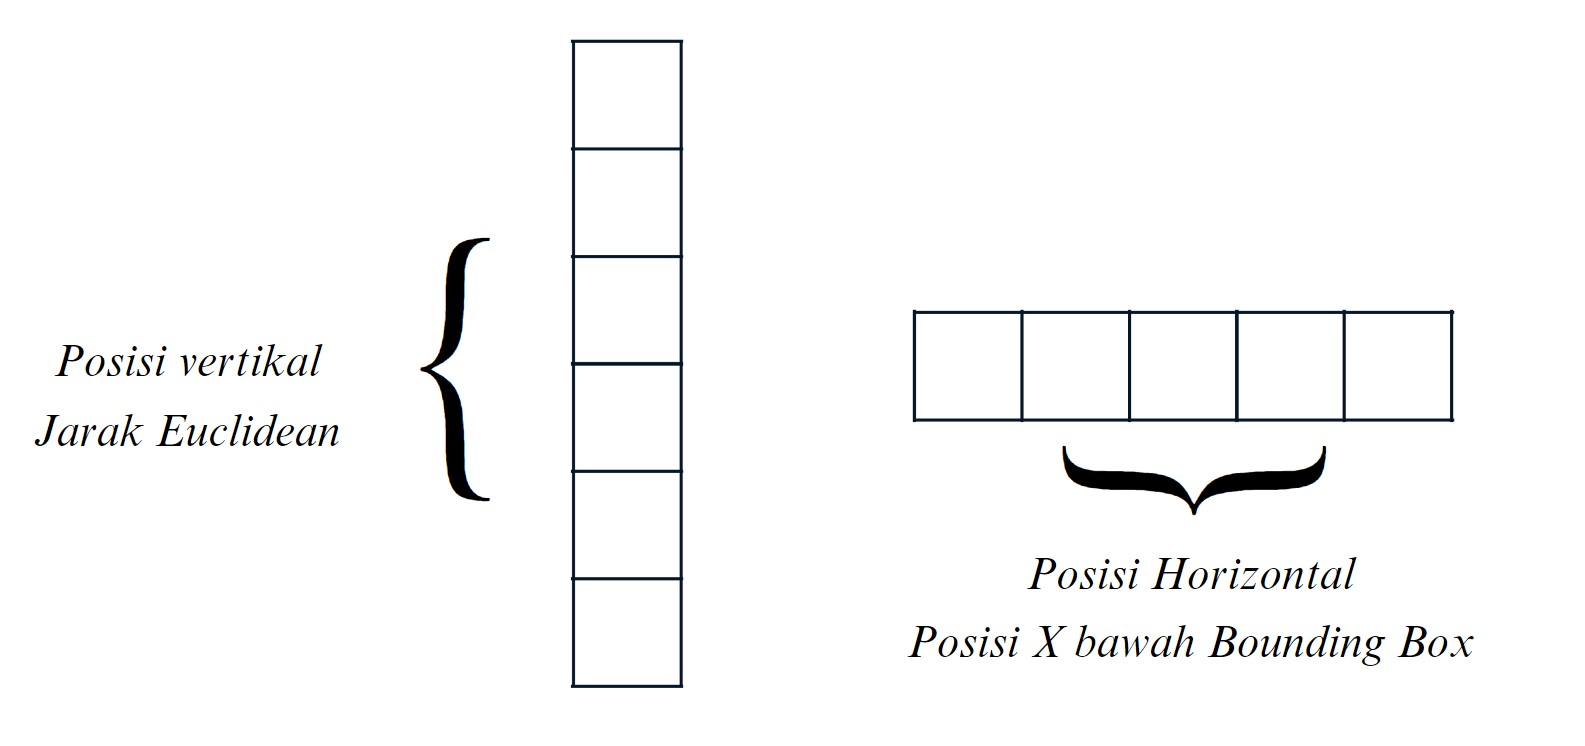
\includegraphics[scale=0.3]{gambar/posisi.jpg}
  % Ubah dengan keterangan gambar yang diinginkan
  \caption{Variabel Dalam perpindahan Posisi terhadap Grid.}
  \label{fig:Kategori Posisi berdasarkan index.}
\end{figure}

Berdasarkan Perhitungan rumus yang tadi didapatkan maka obstacle yang dideteksi dapat dipetakan posisinya relatif terhadap sumbu x dan y pada grid. Dimana keputusan mengambil variabel tersebut didasari oleh visibilitas hasil deteksi dan performa model dari hasil training. sehingga posisi yang dipetakan akan menjadi lebih akurat dan pengambilan keputusan dapat lebih konsisten. Namun dari posisi tersebut grid masih belum dapat merepresentasikan besar objek yang akan dilalui sehingga diperlukanlah sebuah variabel tambahan yang dapat membuat grid menggambar lebar objek relatif terhadap pixel yang nantinya akan dipetakan dalam grid. sehingga pada contoh gambar selanjutnya akan dijabarkan pemetaan lebar objek pada grid.

\begin{figure}[H]
  \centering
  % Ubah dengan nama file gambar dan ukuran yang akan digunakan
  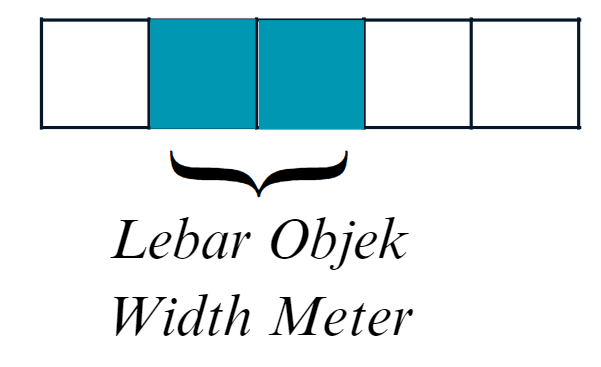
\includegraphics[scale=0.3]{gambar/Lebarobjek.png}
  % Ubah dengan keterangan gambar yang diinginkan
  \caption{Lebar Objek dalam grid.}
  \label{fig:Lebar Objek dalam grid.}
\end{figure}

Dapat dilihat pada gambar diatas pemetaan lebar berdasarkan nilai yang didapatkan pada variabel width meter. Dimana sesuai dengan parameter ukuran kotak yang telah ditentukan. Maka untuk setiap penambahan 0.2 meter ukuran lebar hasil deteksi yang didapatkan akan menambah jumlah kotak yang akan ditampilkan. 

Adapun beberapa kondisi dimana perlu dilakukannya kalibrasi mengingat bounding box yang ditampilkan tidak sepenuhnya dapat dengan akurat merepresentasikan posisi objek dalam horizontal sehingga perlunya ditambahkan sebuah nilai kalibrasi yang akan berperan dalam mengatasi limitasi bounding box yang kadang memiliki nilai tengah yang tidak konsisten. Penambahan nilai pada rumus dibawah dapat menyesuaikan nilai posisi x pada grid agar lebih mendekati nilai kenyataan.

\begin{equation}
    Grid\_x = (\frac{posisi\_x\_bounding\_box +konstanta}{scale\_factor})
\end{equation}

Setelah pemetaan grid dilakukan selanjutnya akan ditampilkan parameter yang akan digunakan dalam pengambilan keputusan belok kursi roda.

\subsection{Output Hasil deteksi}
Dalam menentukan keputusan dalam pembelokan kursi roda akan ditambahkan beberapa parameter. Parameter ini berfungsi untuk menentukan Kapan kursi roda harus berbelok dan seberapa jauh kursi roda harus berbelok. Parameter tersebut akan dibagi menjadi beberapa status yang dimana kondisi-kondisi yang telah ditetapkan harus terpenuhi untuk dapat dikatakan memenuhi syarat.

\subsubsection*{1. Valid Object Condition}
Pada kondisi ini objek harus terdeteksi pada input citra untuk memenuhi kondisi ini. Tidak ada parameter khusus yang mengharuskan kursi roda untuk berbelok dalam kondisi ini, karena posisi kursi roda masih tergolong jauh dari posisi hasil deteksi. Dimana pengambilan keputusan yang akan dilakukan kursi roda adalah untuk tetap maju. Berikut merupakan contoh gambar untuk kondisi yang memenuhi. 

\begin{figure}[H]
  \centering
  % Ubah dengan nama file gambar dan ukuran yang akan digunakan
  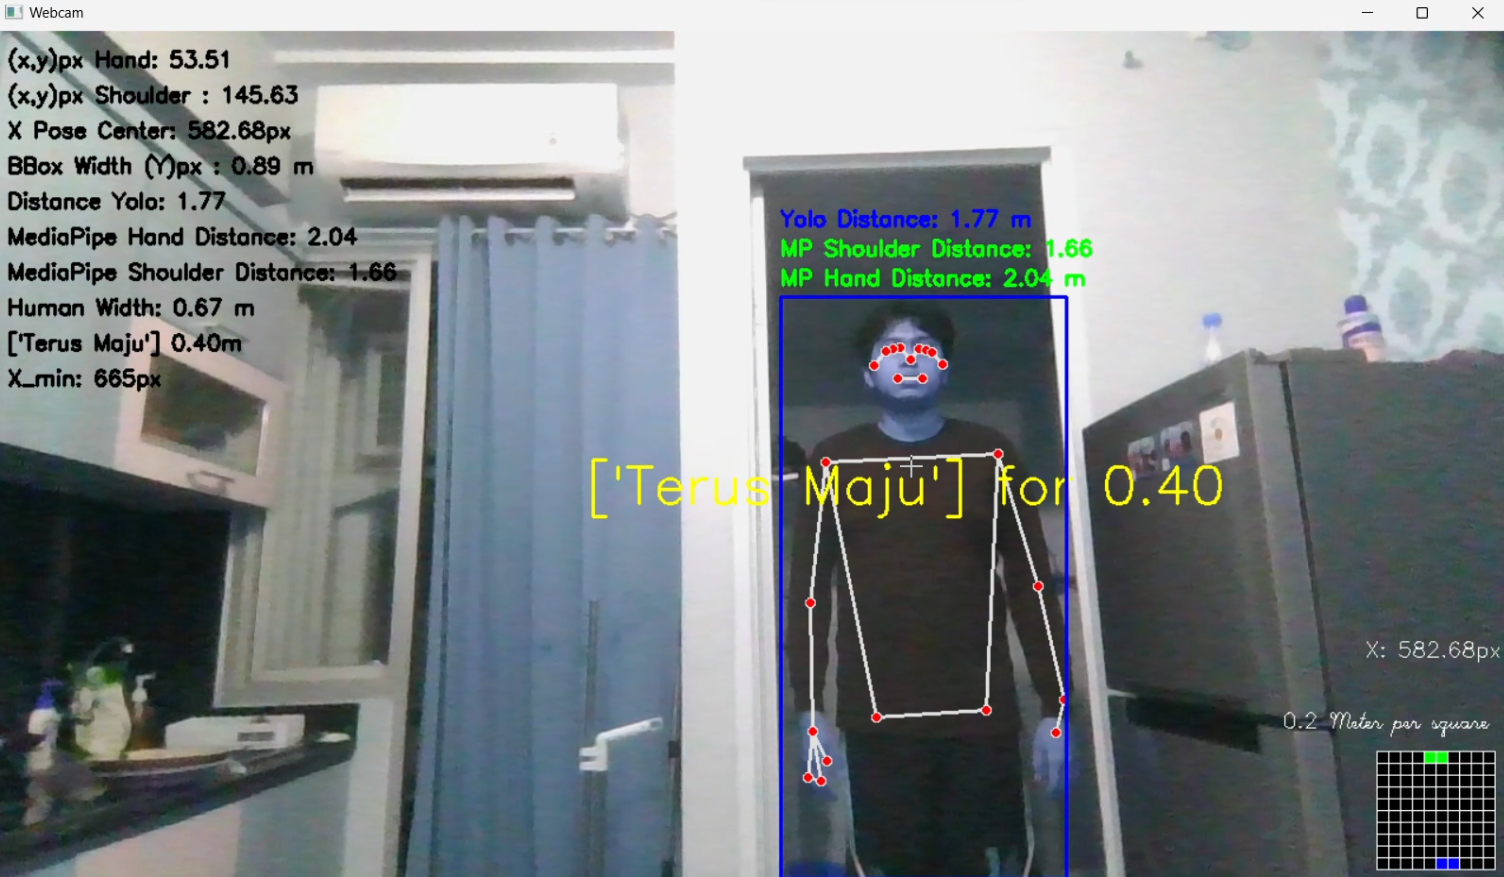
\includegraphics[scale=0.3]{gambar/posisibiru.png}
  % Ubah dengan keterangan gambar yang diinginkan
  \caption{Contoh valid object diatas 0.8 Meter.}
  \label{fig:Valid object diatas 0.8 Meter.}
\end{figure}

Dapat dilihat pada gambar diatas dimana objek hanya terdeteksi namun belum terdapat indikasi mendesak untuk kursi roda dalam mengambil keputusan karena posisi hasil deteksi yang masih tergolong jauh. adapun warna bounding box yang digambar berwarna biru sebagai penanda objek tergolong \emph{safe distance} terhadap kursi roda. Sehingga instruksi yang akan dikirim adalah tetap maju. 

\begin{figure}[H]
  \centering
  % Ubah dengan nama file gambar dan ukuran yang akan digunakan
  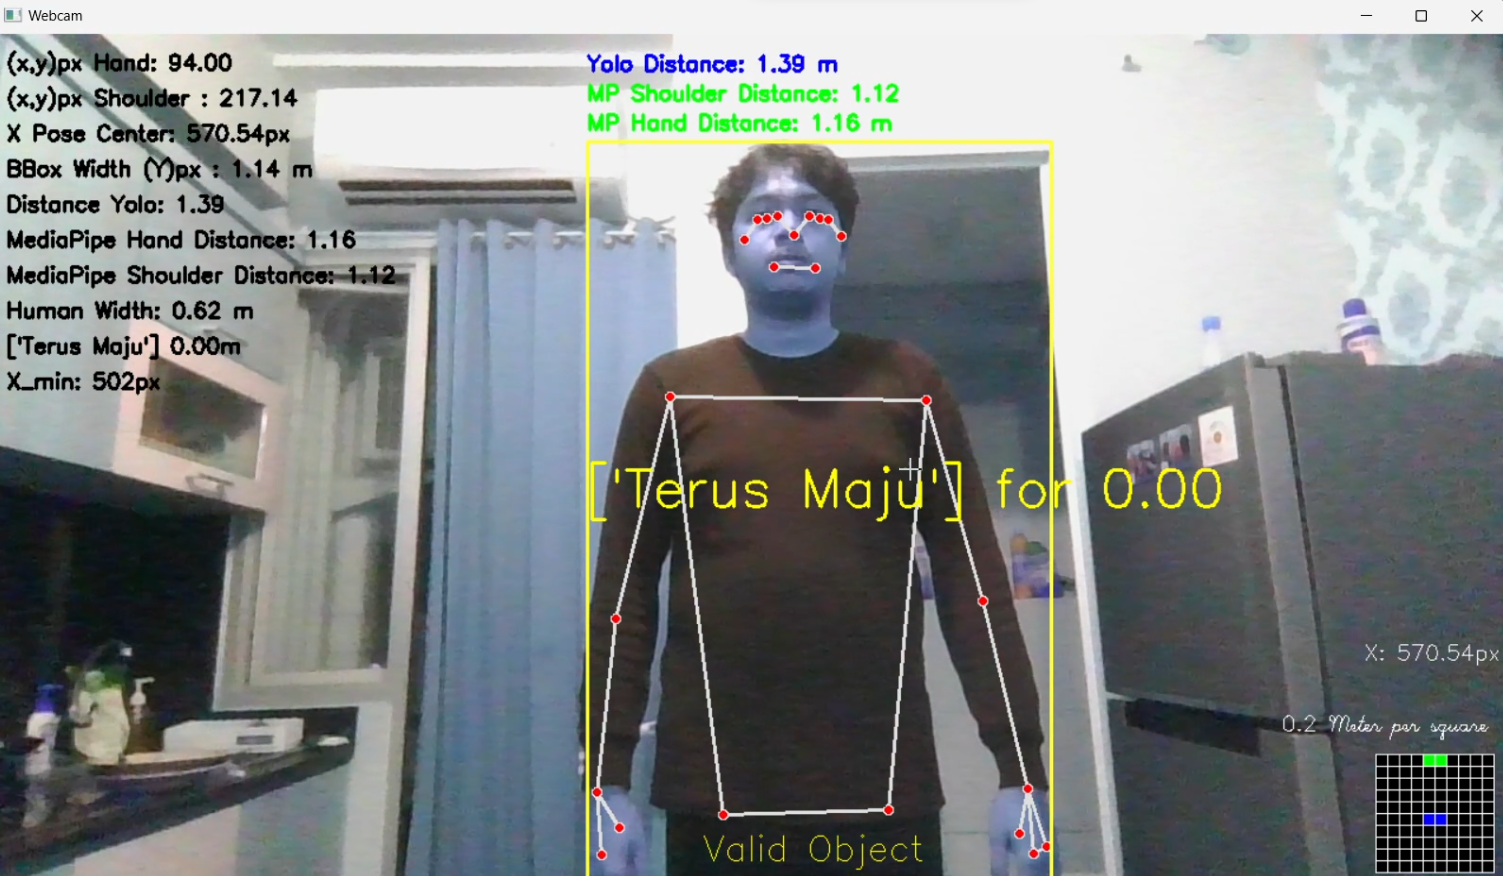
\includegraphics[scale=0.3]{gambar/posisikuning.png}
  % Ubah dengan keterangan gambar yang diinginkan
  \caption{Contoh valid object dibawah 0.8 Meter.}
  \label{fig:Valid object diatas 0.8 Meter.}
\end{figure}

Saat hasil objek yang terdeteksi menjadi lebih dekat terhadap kursi roda maka bounding box akan berubah menjadi warna kuning yang menjadi indikasi bahwa objek yang terdeteksi sudah dibawah 0.8 Meter. sejauh ini pengambilan keputusan untuk belok belum dilakukan, namun akan menampilkan "valid object" pada bagian bawah layar kamera. Mengindikasikan objek benar-benar terdeteksi dan mulai mendekati. Dapat dilihat juga pada Grid di pojok kanan bawah bahwa perpindahan telah terjadi yang direpresentasikan berdasarkan perhitungan variabel yang ditampilkan pada pojok kanan atas layar kamera. Adapun beberapa contoh lainnya dapat dilihat digambar berikut.

\begin{figure}[H]
  \centering
  % Ubah dengan nama file gambar dan ukuran yang akan digunakan
  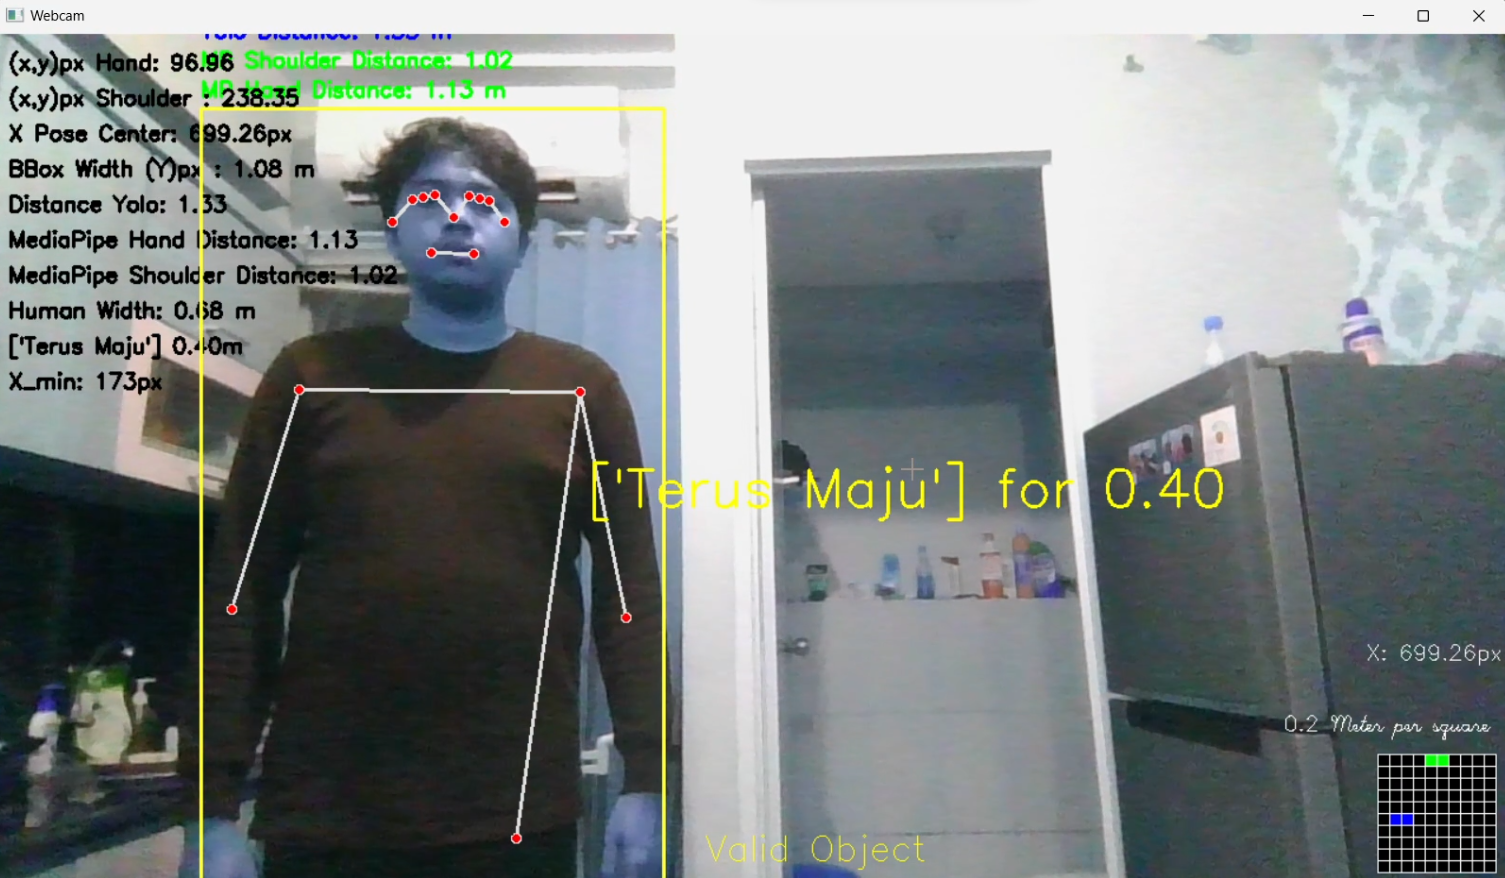
\includegraphics[scale=0.3]{gambar/posisikuning kiri.png}
  % Ubah dengan keterangan gambar yang diinginkan
  \caption{Contoh lain valid object dibawah 0.8 Meter condong kiri.}
  \label{fig:Contoh lain Valid object dibawah 0.8 Meter.}
\end{figure}

\begin{figure}[H]
  \centering
  % Ubah dengan nama file gambar dan ukuran yang akan digunakan
  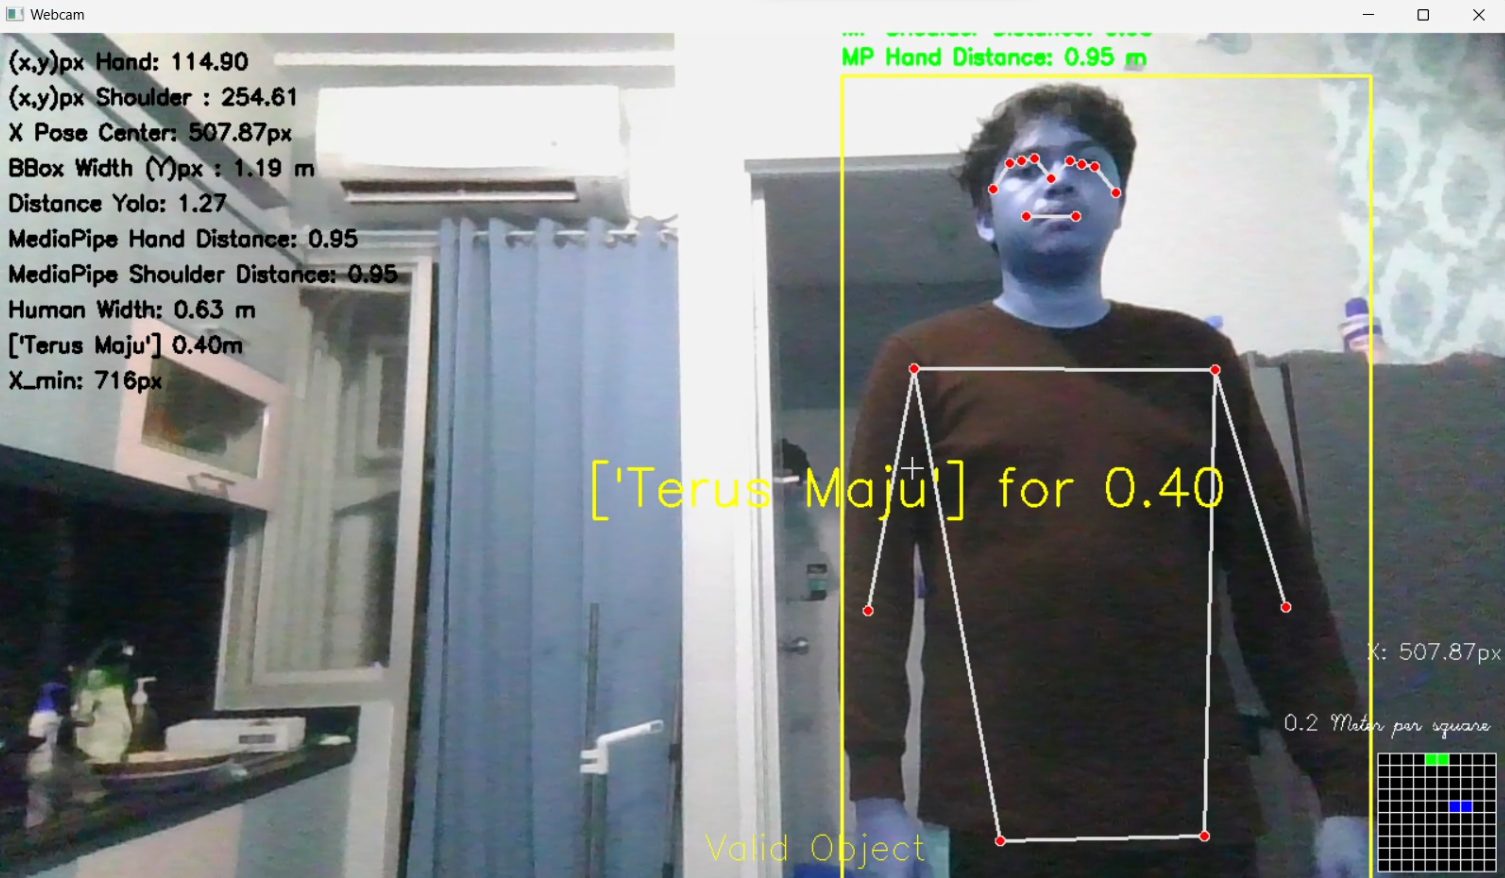
\includegraphics[scale=0.3]{gambar/posisikuning kanan.png}
  % Ubah dengan keterangan gambar yang diinginkan
  \caption{Contoh lain valid object dibawah 0.8 Meter condong kanan.}
  \label{fig:Valid object dibawah 0.8 Meter.}
\end{figure}

\subsubsection{2. Near Object Condition}
Pada kondisi ini objek harus terdeteksi pada input citra untuk memenuhi kondisi ini dan objek harus berada dibawah 0.5 Meter jarak terdeteksi. Dalam kondisi ini akan dibagi menjadi 3 pengambilan keputusan. yaitu sebagai berikut: 

\subsubsection*{Hasil deteksi objek pada grid menunjukan Index Kiri Lebih besar dari Index kanan}
Pada kondisi ini posisi hasil deteksi menunjukan nilai yang lebih besar pada Index kiri (Index 1-5) yang berarti bahwa objek sedang berada pada sebelah kiri posisi terhadap kursi roda. Dapat dilihat pada contoh gambar dibawah.

\begin{figure}[H]
  \centering
  % Ubah dengan nama file gambar dan ukuran yang akan digunakan
  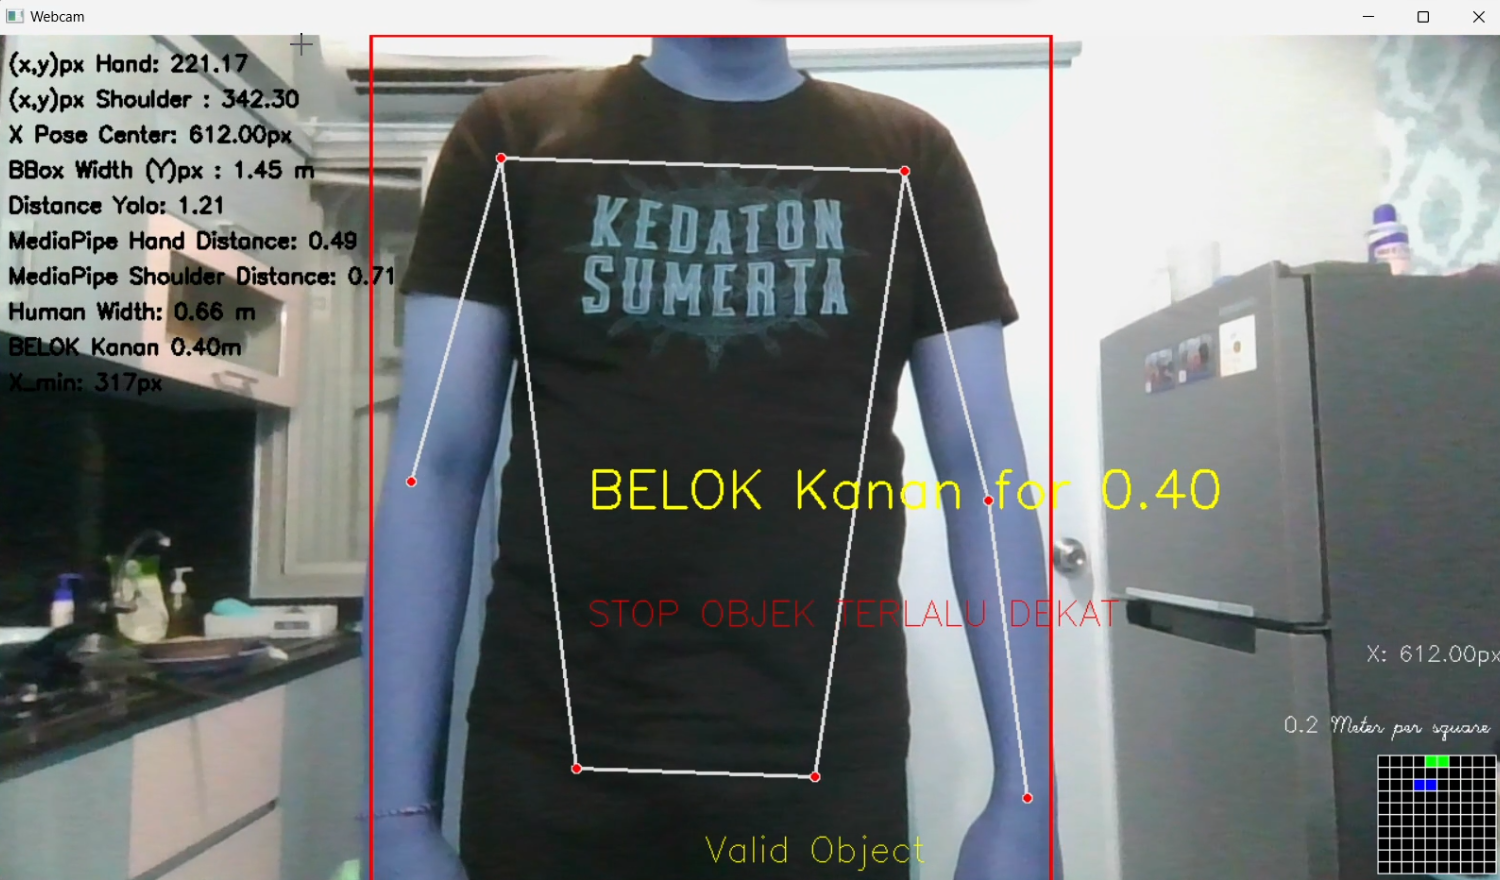
\includegraphics[scale=0.3]{gambar/merahkiri.png}
  % Ubah dengan keterangan gambar yang diinginkan
  \caption{Contoh kondisi Near Object Index Kiri \textgreater Kanan .}
  \label{fig:Valid object dibawah 0.8 Meter.}
\end{figure}

Dapat dilihat pada gambar, grid nilainya lebih mengarah index kiri dari pada kanan. Dimana dilihat dari pertimbangan posisi tersebut maka kursi roda akan menghindar ke Kanan yang merupakan belokan yang lebih aman ketimbang belokan ke kiri.

\subsubsection*{Hasil deteksi objek pada grid menunjukan index Kanan lebih besar dari Index kiri}
Pada kondisi ini posisi hasil deteksi menunjukan nilai yang lebih besar pada index kanan (6-10) yang berarti bahwa objek sedang berada pada sebelah kanan posisi terhadap kursi roda. dapat dilihat pada contoh gambar dibawah

\begin{figure}[H]
    \centering
    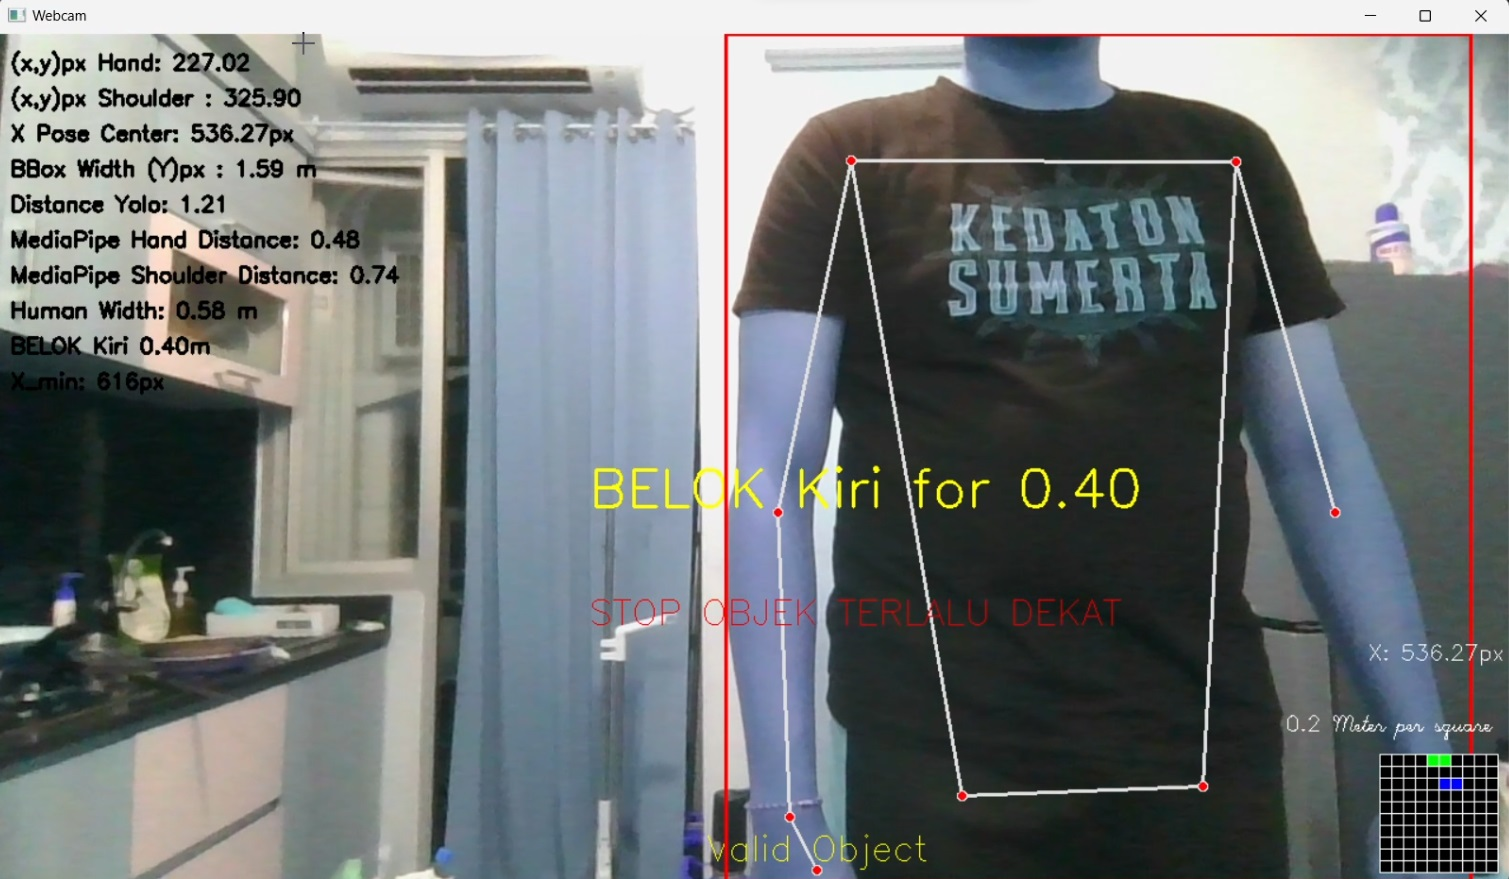
\includegraphics[scale=0.3]{gambar/merahkanan.jpg}
    \caption{Contoh kondisi Near Object Index Kanan \textgreater kiri}
    \label{fig:Near Object index kanan>kiri}
\end{figure}

Dapat dilihat pada gambar, grid nilainya lebih mengarah index kanan dari pada kiri. Dimana dilihat dari pertimbangan posisi tersebut maka kursi roda akan menghindar ke kiri yang merupakan belokan yang lebih aman ketimbang belokan ke kanan.

\subsubsection*{Hasil deteksi objek pada grid menunjukan posisi Linear terhadap kursi roda}
Pada kondisi ini perlu ditambahkan sebuah perintah untuk pengambilan keputusan dimana posisi belok pada kondisi ini baik melalui kanan maupun kiri tidak akan memiliki kelebihan/kekurangan karena dalam posisi ini nilai index sama besarnya baik kanan maupun kiri. sehingga perlu dilakukan pendekatan yang baik agar pengambilan keputusan ini tidak menimbulkan kesalahan. Pada tugas proyek ini pengambilan keputusan ini didasari pada nilai random. Sehingga keputusan yang diambil bisa ke kanan maupun ke kiri. 

\begin{figure}[H]
    \centering
    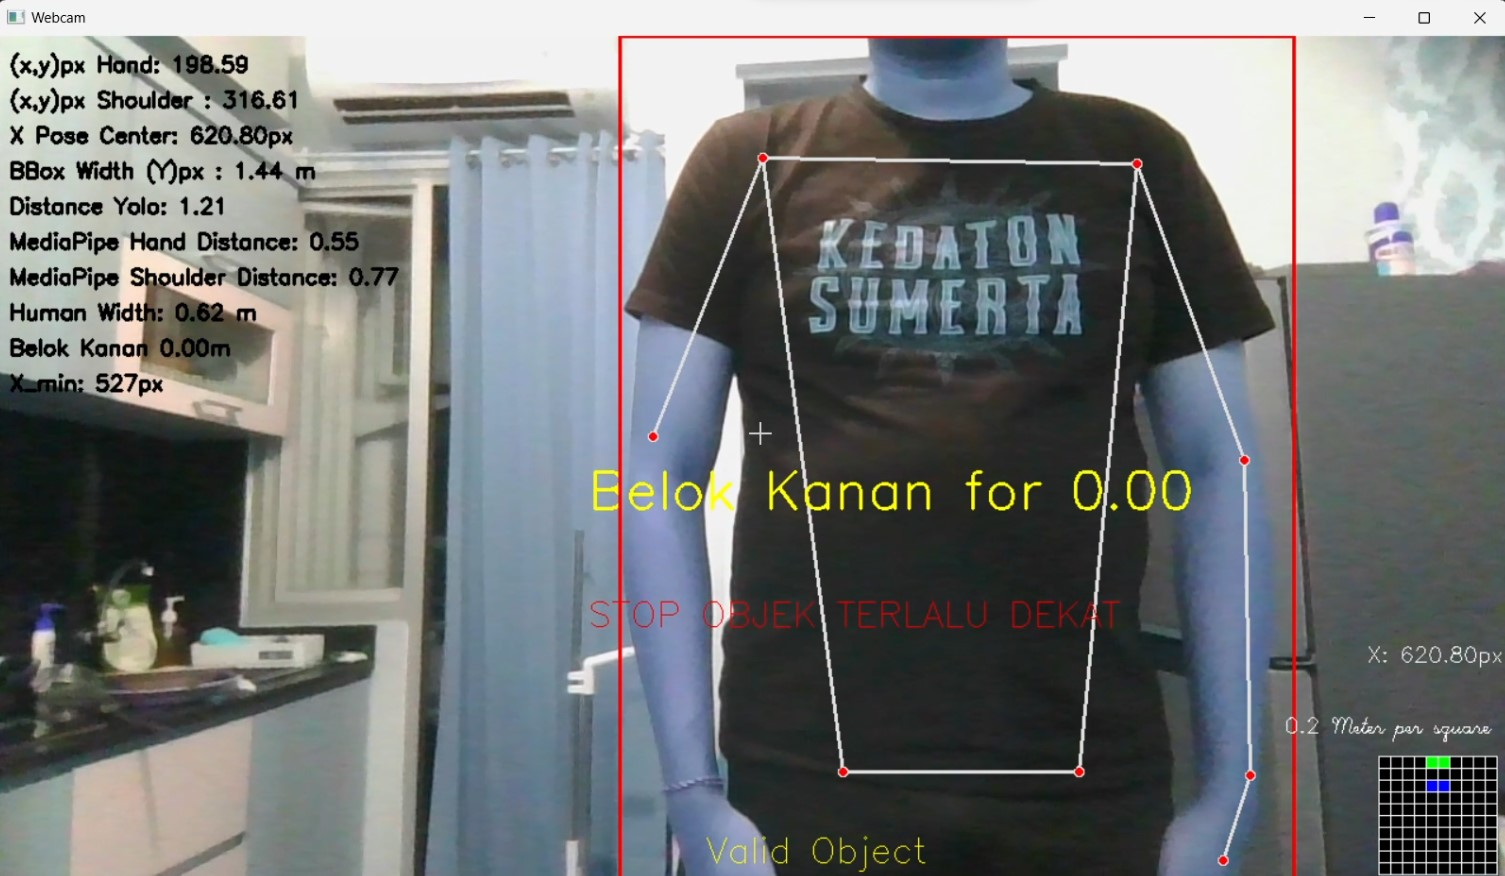
\includegraphics[scale=0.3]{gambar/merahlinier.jpg}
    \caption{Contoh kondisi Near Object Liniear.}
    \label{fig:Near Object Linear}
\end{figure}

Dapat dilihat pada gambar, gridnya sejajar dengan posisi kursi roda. Sehingga penggunaan random akan sangat berguna untuk mengabil keputusan apabila menghadapi kasus seperti ini.


\cleardoublepage

% Bab 4 pengujian dan analisis
\chapter{PENGUJIAN DAN ANALISIS}
\label{chap:pengujiananalisis}

% Ubah bagian-bagian berikut dengan isi dari pengujian dan analisis

Pada penelitian ini dilakukan uji dan analisis dari model prediksi yang sudah dibuat. Pengujian ini dilakukan dengan beberapa skenario pengujian. Dalam pengujian ini akan diambil data yang akan merujuk pada performa sistem yang telah dibuat. Data - data yang diambil juga akan divisualisasikan untuk mendapatkan indikasi terkait hasil tugas akhir yang telah dilakukan.

\section{Pengujian}
\label{sec:skenariopengujian}

Pada subbab ini dilakukan beberapa skenario pengujian terhadap model untuk mengetahui performa dan tingkat kesalahan yang dapat membuka kesempatan pengembangan penelitian di masa depan serta menarik kesimpulan secara keseluruhan. Berikut adalah skenario pengujian yang dilakukan.

\subsection{Hasil Pengujian Performa menggunakan YOLOV8}
Dalam pembuatan model yang digunakan, dilakukan pengambilan dan labeling data citra yang akan digunakan sebagai set data pelatihan atau set data \emph{train}. Dimana data yang digunakan pada sistem yang akan dibuat menggunakan data citra manusia yang telah dijabarkan pada bab sebelumnya.

Data yang digunakan sebagai set data berjumlah  1735 data citra manusia. Dalam pengembangan model nantinya data citra ini akan dibagi menjadi 2 bagian dimana sebesar 1435 data citra sebagai set pelatihan dan sisanya sebesar 300 data citra akan digunakan sebagai set validasi. Setelah proporsi dataset ditentukan maka API key akan digenerate pada roboflow yang nantinya akan dipanggil untuk dilakukan proses training. 

Setelah proses pemuatan set dilakukan, maka akan dilajutkan pada proses training model. Proses training dilakukan dengan menggunakan beberapa parameter, yang dimana parameter ini akan dibandingkan performanya melalui nilai confusion matrix maupun nilai akurasi deteksi seperti presisi , recall, mapupun classification loss.

Pelatihan pertama menggunakan 100\emph{epoch} dan \emph{batch size} sebesar 16 dengan tindakan praproses merubah ukuran gambar pada dataset menjadi 800x800 piksel dengan pemberian augmentasi berupa 90\textdegree rotasi dan noise. Penggunaan augmentasi ini menambah jumlah data citra yang semulanya 1435 menjadi 4305. Adapun tujuan dari pelatihan ini untuk mengetahui seberapa baik peningkatan model pre- trained yang digunakan dalam deteksi manusia dengan menggunakan dataset yang teraugmentasi.

Didapatkan nilai box loss pada proses training menggunakan YOLOV8 ini adalah sebesar 0.819 setelah 100 epoch. Box loss mengukur seberapa baik model memprediksi bounding boxes seputar objek. Loss ini umumnya dihitung menggunakan metode seperti Intersection over Union (IoU) atau variasinya seperti CIoU atau DIoU, yang mengukur kesesuaian antara bounding box yang diprediksi dengan ground truth. Tujuan dari loss ini adalah untuk mengoptimalkan model agar bounding box yang diprediksi sesuai dengan posisi dan ukuran objek sebenarnya dalam gambar. Adapun penurunan yang nilai box loss yang didapatkan selama training menandakan bahwa hasil training yang dilakukan telah berhasil membuat model menentukan koordinat bounding box pada object manusia dengan akurat.

Didapatkan nilai box loss pada proses validasi menggunakan YOLOV8 ini sebesar 1.2 , adapun box loss pada validasi ini mengindikasikan kemampuan mengenali objek pada data uji. Secara teori, penurunan object loss pada tahap validasi menandakan bahwa model mampu melakukan deteksi objek secara umum. bukan hanya pada data pelatihan.

Skor mAP pada threshold 0.5 yang diperoleh pada proses ini adalah sebesar 80.9\% dimana nilai ini mengindikasikan bahwa model memiliki kemampuan yang baik untuk mendeteksi objek dengan ketepatan yang tinggi, dengan syarat kriteria IoU minimal 0.5 terpenuhi. Ini mengindikasikan dalam banyak percobaan kasus, bounding box yang diprediksi oleh model memiliki overlap yang signifikan dengan bounding box ground truth.

Nilai nilai yang dicantumkan juga dapat dilihat lebih detail pada visualiasi berikut ini. Dimana nilai visualisasi cenderung turun pada Box loss dan cenderung naik pada skor mAP. 

\begin{figure}[H]
    \centering
    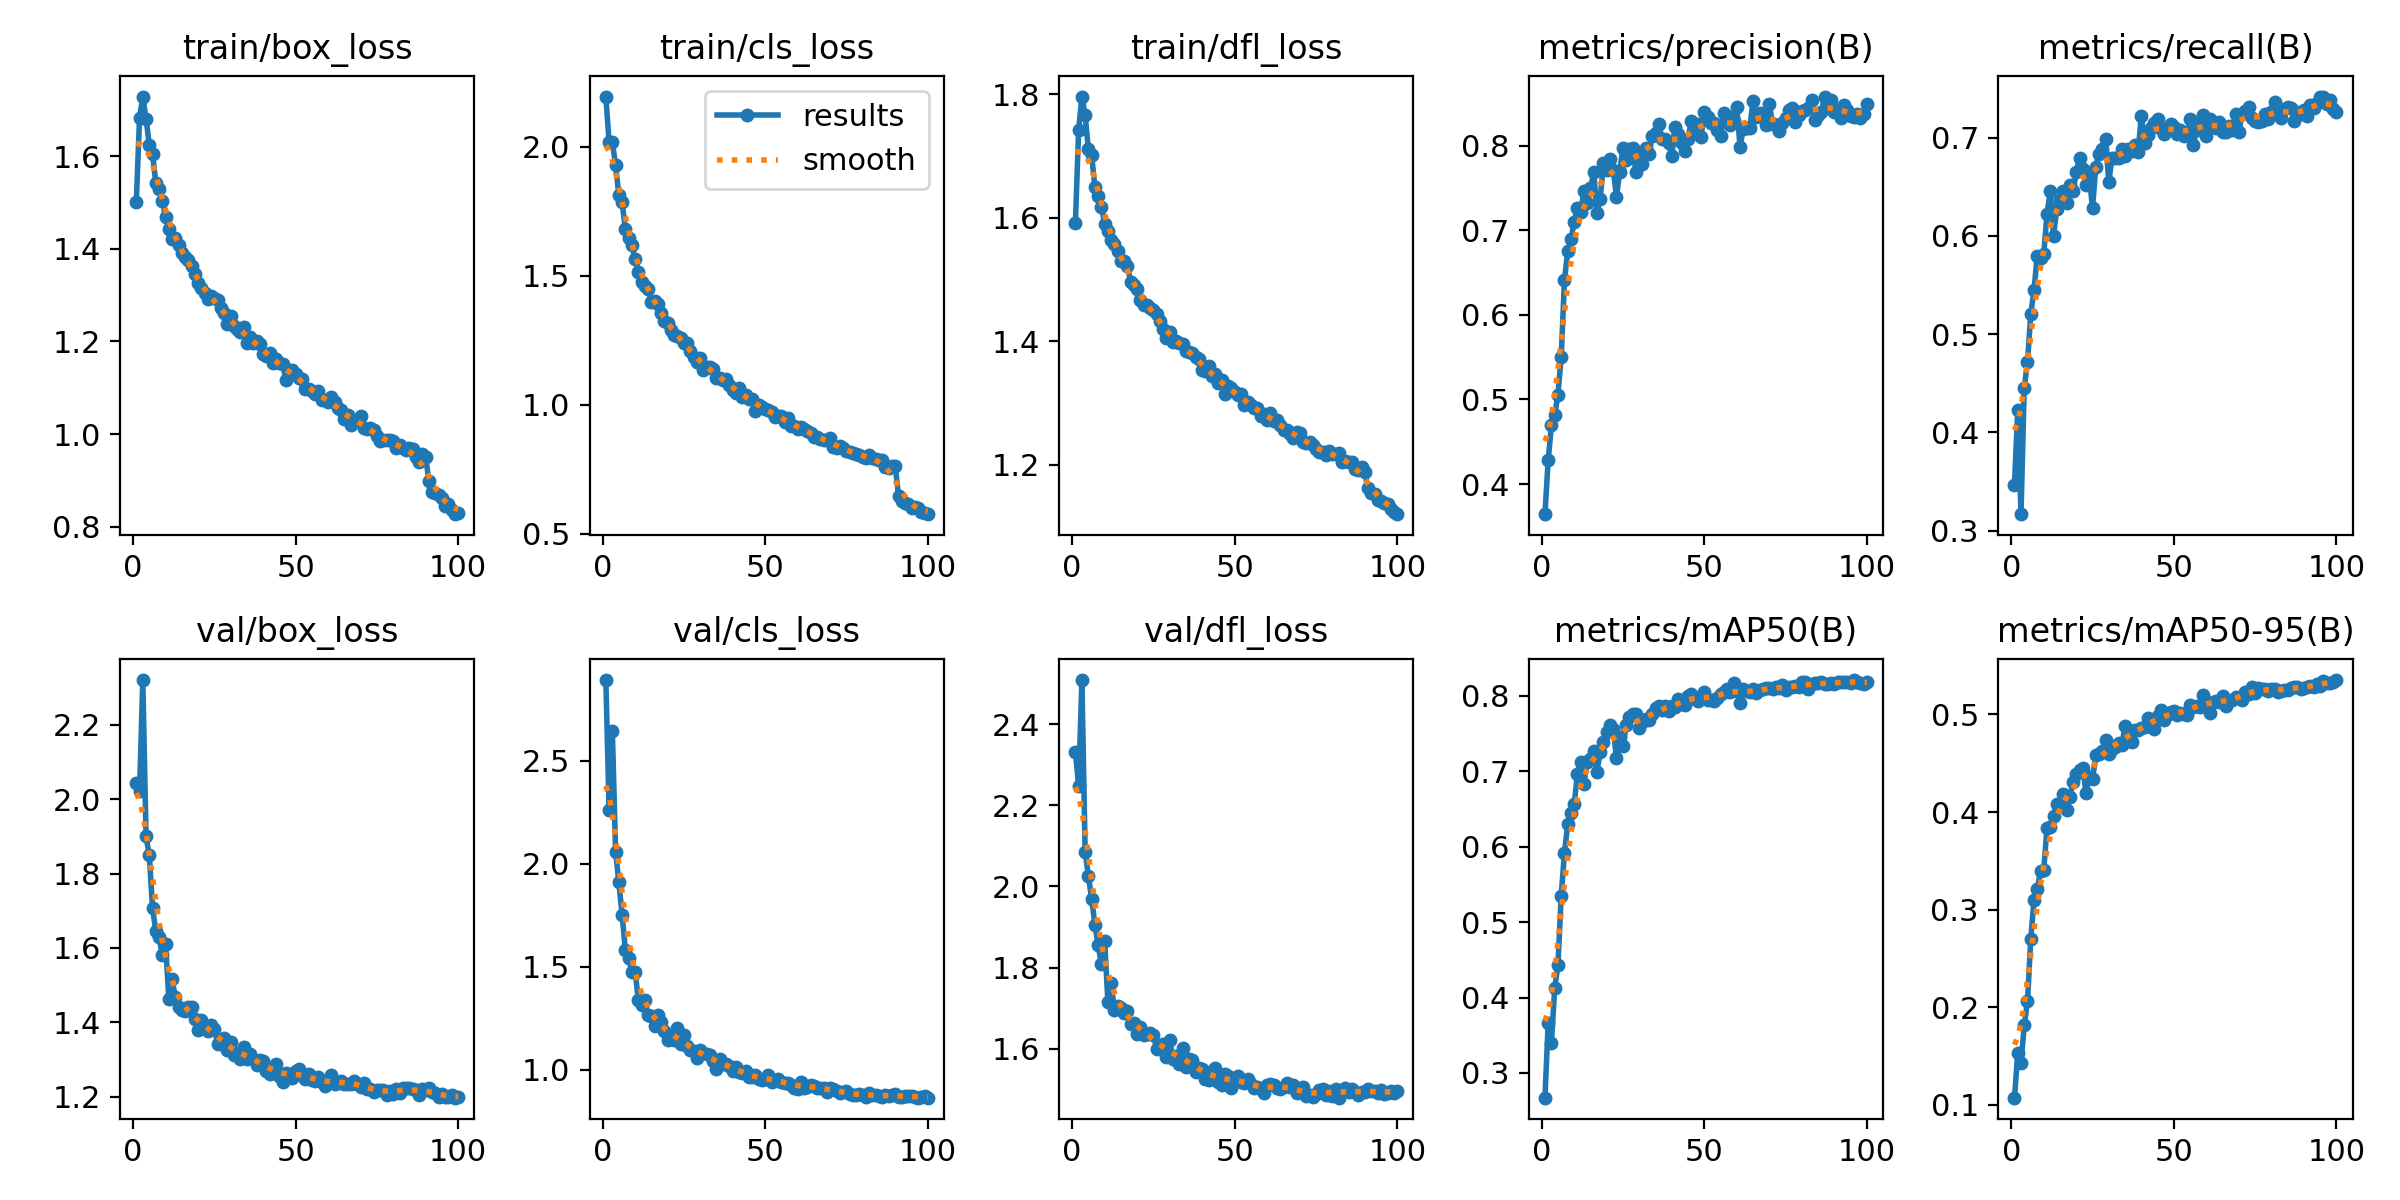
\includegraphics[scale=0.4]{gambar/loss 100 epoch.png}
    \caption{Visualisasi Hasil training}
    \label{fig:visualisasi hasil training}
\end{figure}

Adapun visualisasi melalui confusion matrix yang digunakan, untuk merepresentasikan hasil model lebih detail. Adapun indikator pada confusion matrix pada setiap kotaknya merepresentasikan nilai \emph{true positive}, \emph{false positive}, \emph{false negative}, \emph{true negative} sesuai dengan bahasan pada bab sebelumnya dapat dilihat pada gambar berikut ini. 

\begin{figure}[H]
    \centering
    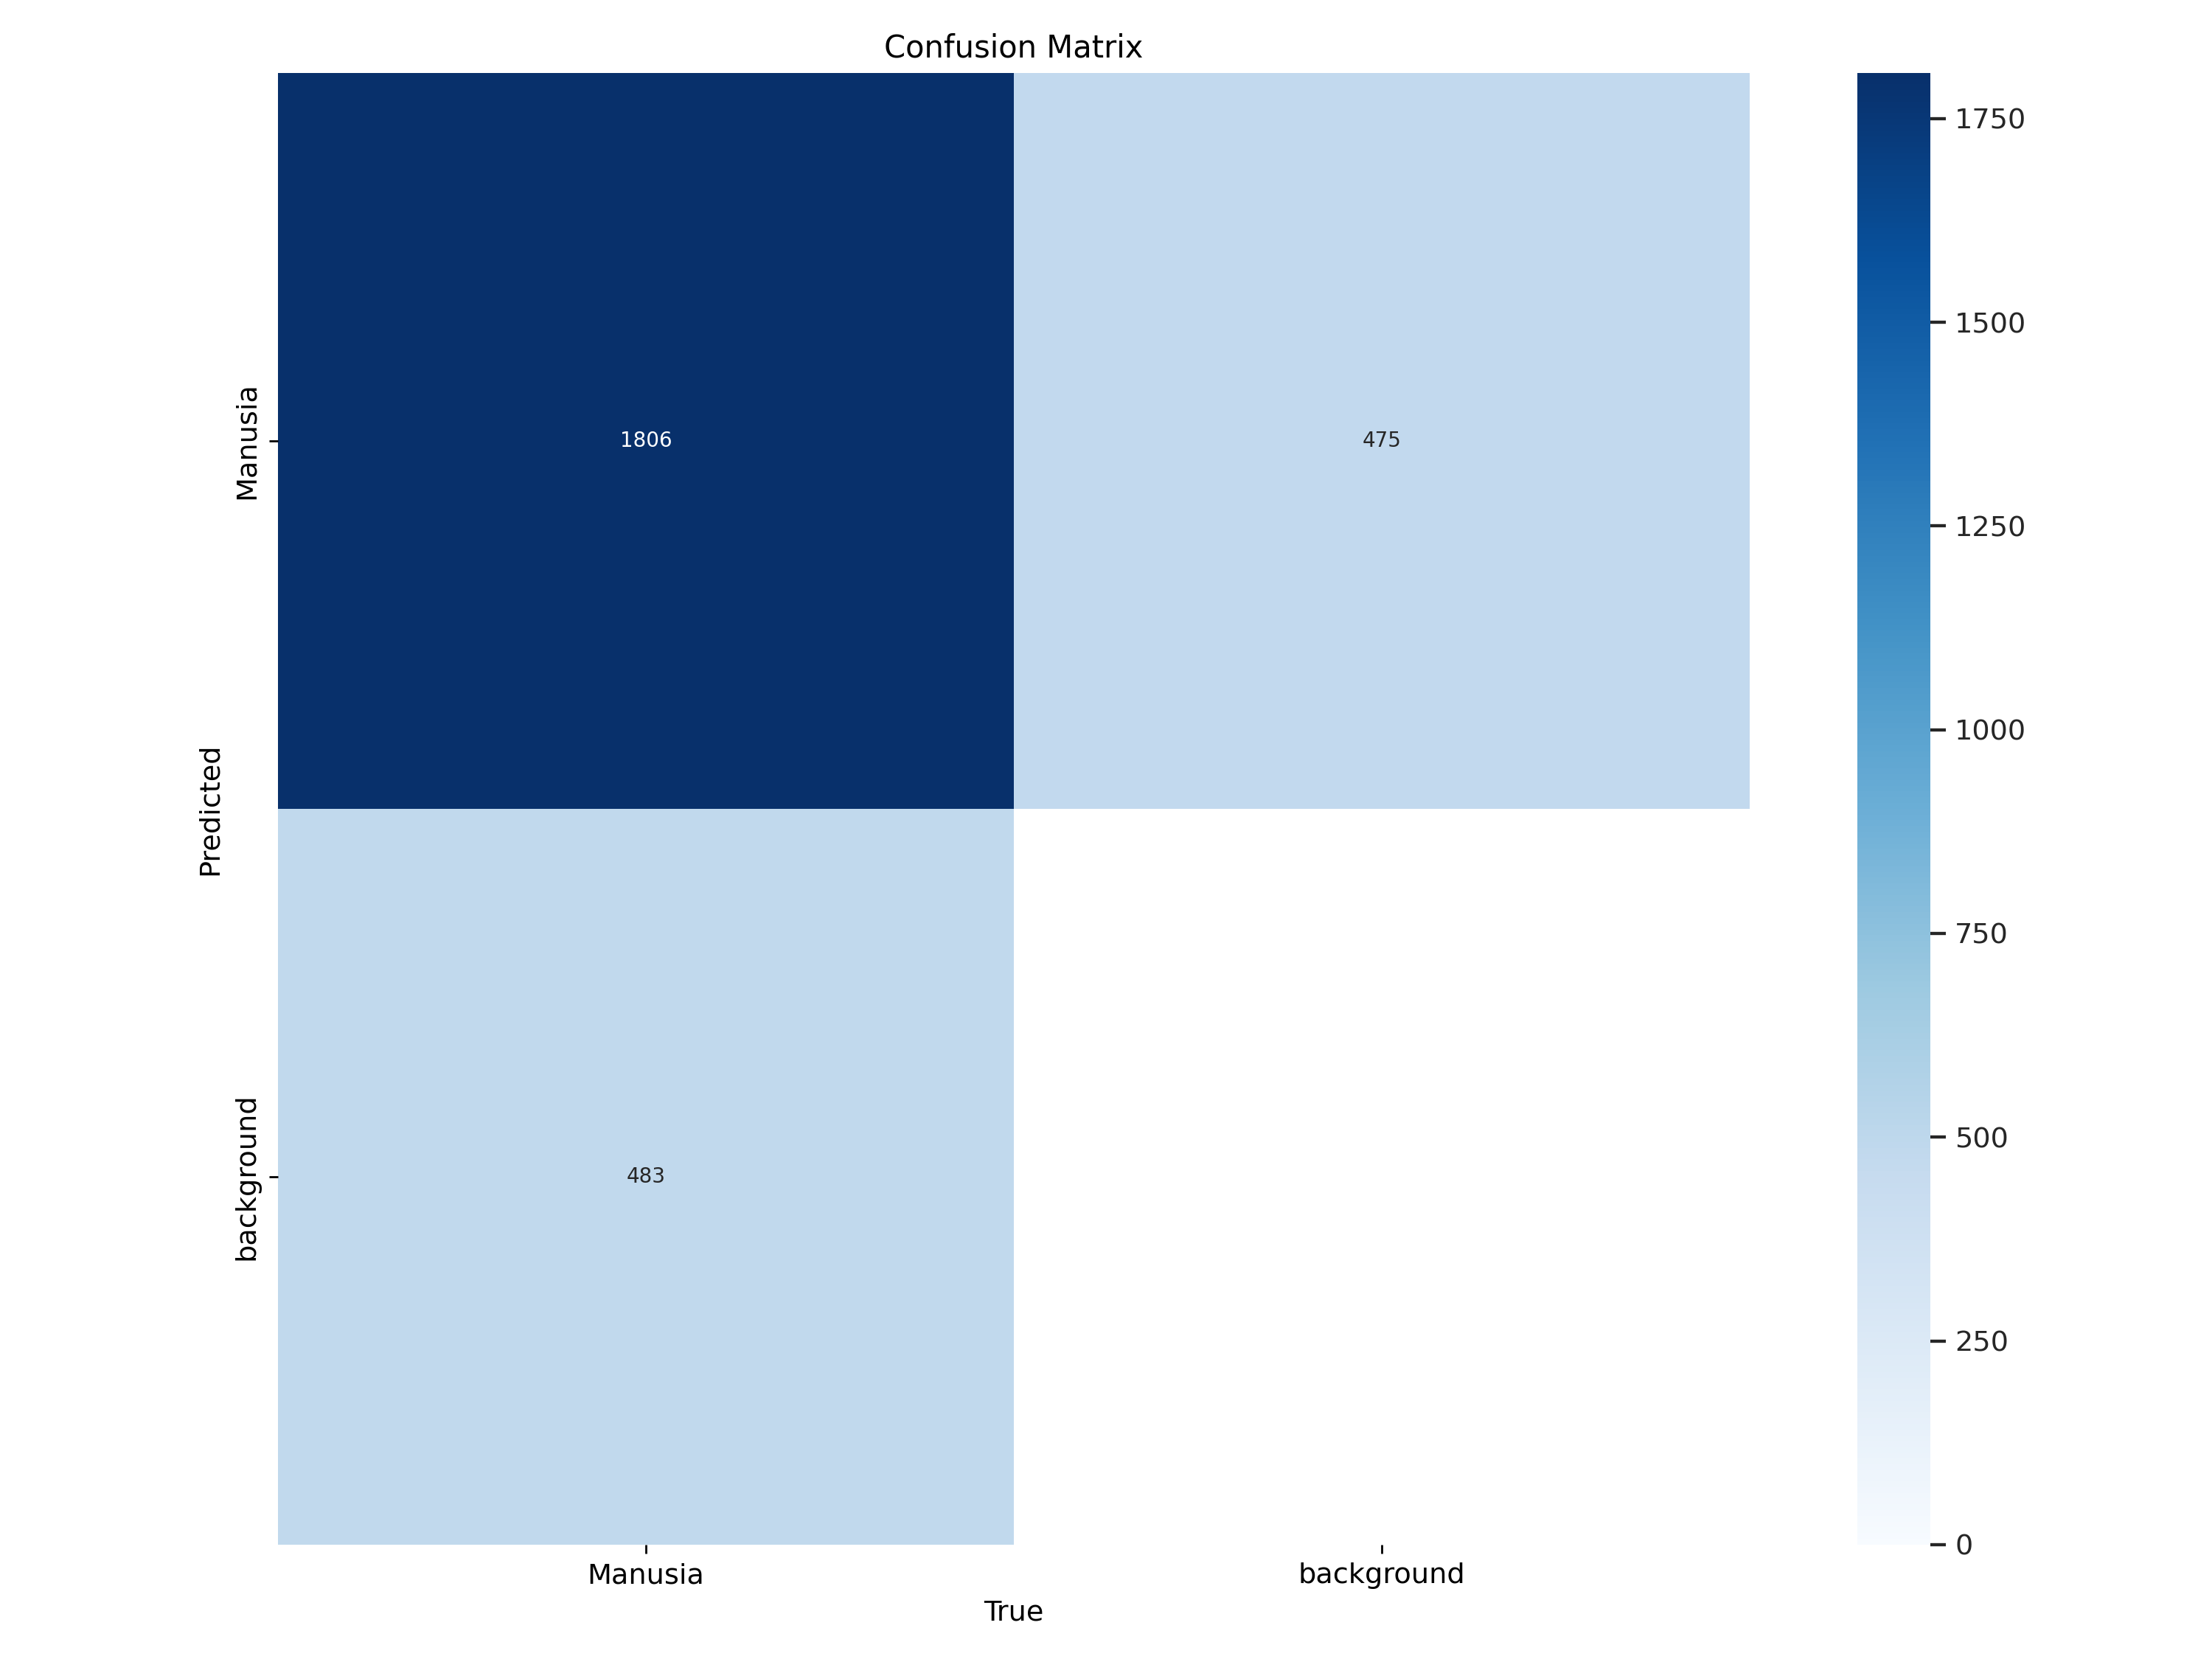
\includegraphics[scale=0.4]{gambar/confusion 100epoch.png}
    \caption{Confusion Matrix Hasil Training}
    \label{fig:visualisasi hasil training}
\end{figure}

Dapat dilihat pada dapat dilihat bahwa dari hasil klasifikasi model terdapat 1806 data citra yang termasuk dalam kategori true positive, 475 citra yang termasuk dalam kategori false positive dan 483 citra yang termasuk false negative.

Dilakukan pula tes inference model yang telah dilatih menggunakan set data test terhadap object manusia. Dapat dilihat pada gambar dibawah nilai confidence score yang cukup tinggi.

\begin{figure}[H]
    \centering
    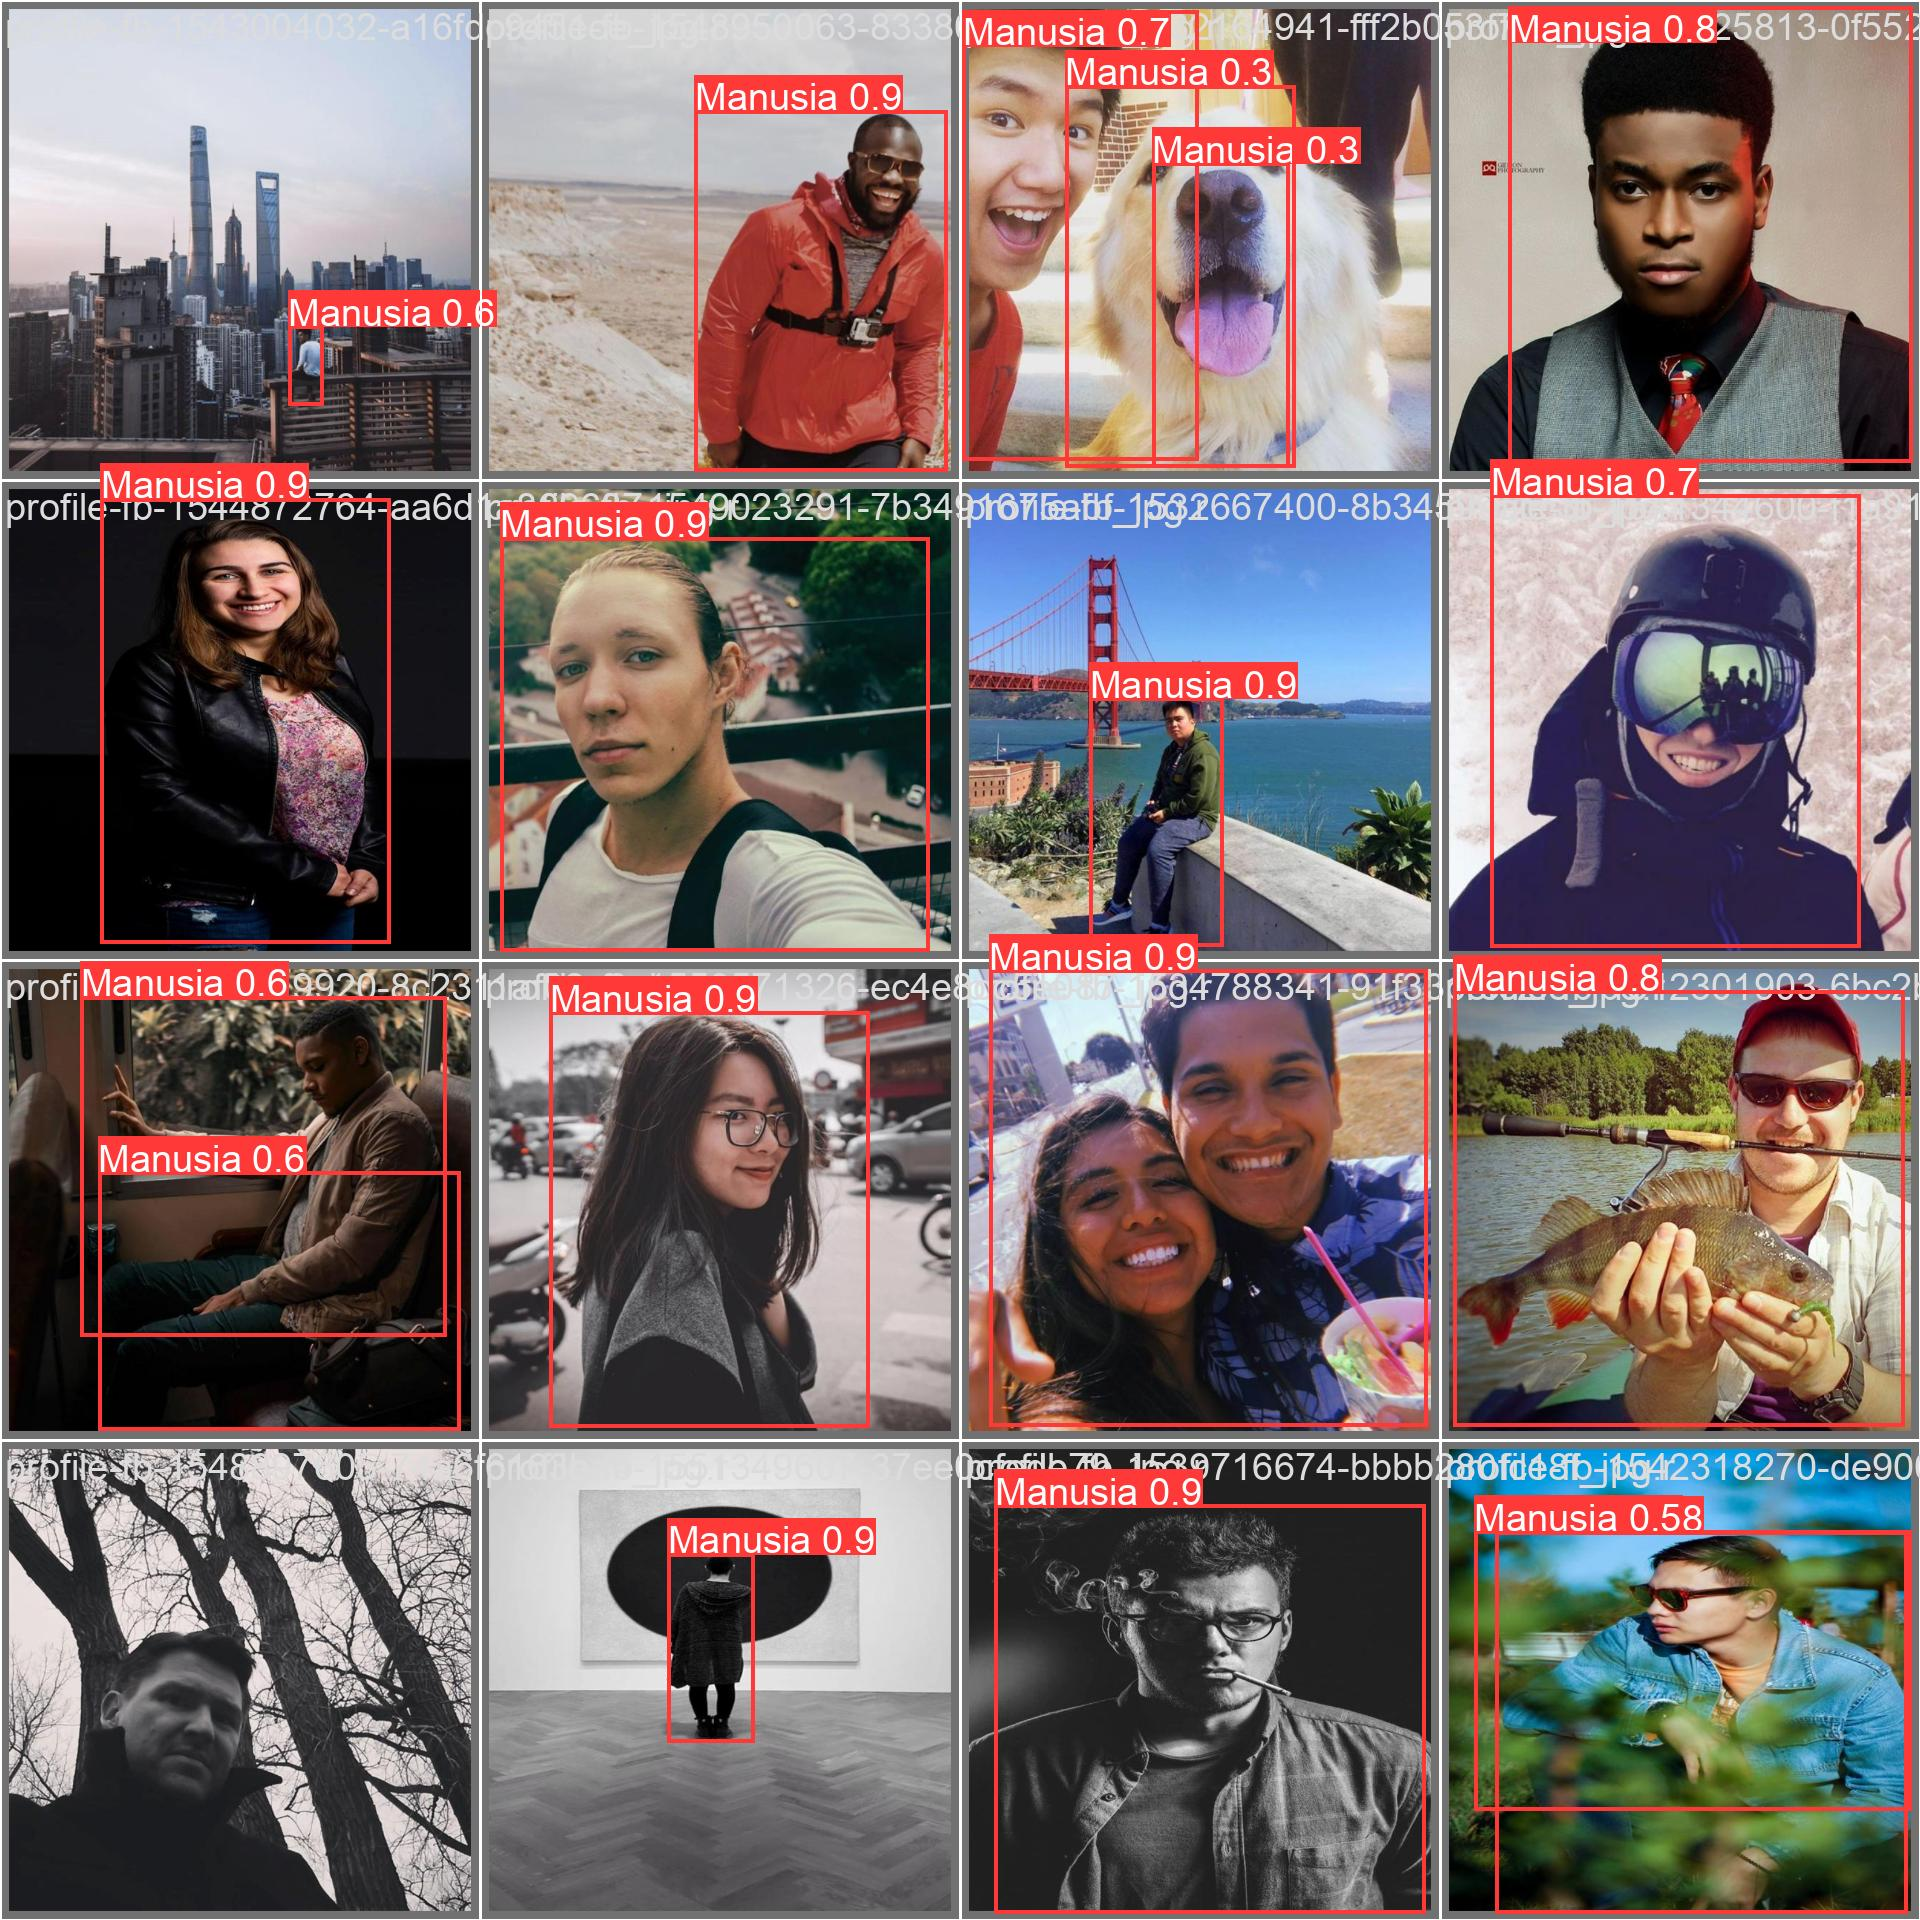
\includegraphics[scale=0.1]{gambar/confiden 100 epoch.jpg}
    \caption{Tes Inferensi Menggunakan Model Terlatih}
    \label{fig:visualisasi hasil training}
\end{figure}

\begin{figure}[H]
    \centering
    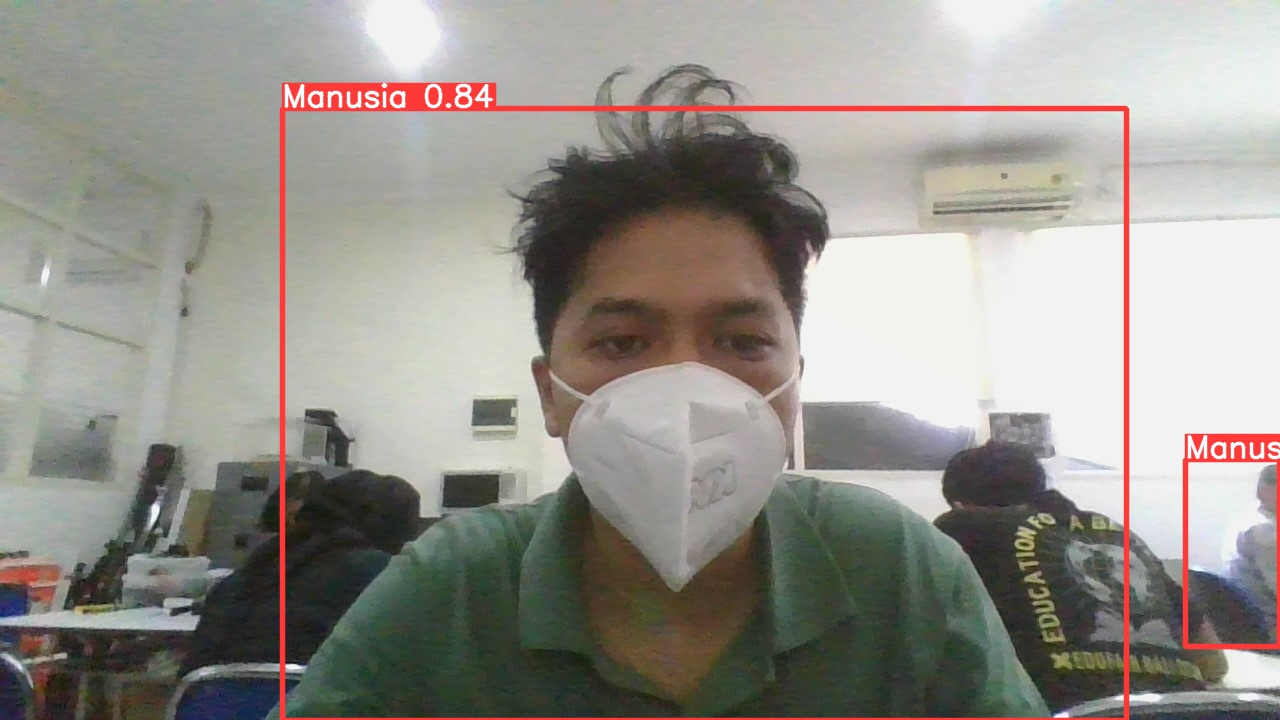
\includegraphics[scale=0.2]{gambar/confiden foto agung 100 epoch.jpg}
    \caption{Tes Inferensi Menggunakan Model Terlatih}
    \label{fig:enter-label}
\end{figure}

Pelatihan kedua menggunakan 150 \emph{epoch} dan \emph{batch size} sebesar 16 dengan tindakan pra proses merubah ukuran gambar pada dataset menjadi 800x800 piksel dengan pemberian augmentasi berupa 90\textdegree rotasi dan noise. Adapun tujuan dari pelatihan ini untuk mengetahui seberapa baik peningkatan model pre- trained yang digunakan dalam deteksi manusia dengan menggunakan dataset yang teraugmentasi.

Didapatkan nilai box loss pada proses training menggunakan YOLOV8 ini adalah sebesar 0.7383 setelah 150 epoch. Box loss mengukur seberapa baik model memprediksi bounding boxes seputar objek. Loss ini umumnya dihitung menggunakan metode seperti Intersection over Union (IoU) atau variasinya seperti CIoU atau DIoU, yang mengukur kesesuaian antara bounding box yang diprediksi dengan ground truth. Tujuan dari loss ini adalah untuk mengoptimalkan model agar bounding box yang diprediksi sesuai dengan posisi dan ukuran objek sebenarnya dalam gambar. Adapun penurunan yang nilai box loss yang didapatkan selama training menandakan bahwa hasil training yang dilakukan telah berhasil membuat model menentukan koordinat bounding box pada object manusia dengan akurat.

Didapatkan nilai box loss pada proses validasi menggunakan YOLOV8 ini sebesar 1.2143, adapun box loss pada validasi ini mengindikasikan kemampuan mengenali objek pada data uji. Secara teori, penurunan object loss pada tahap validasi menandakan bahwa model mampu melakukan deteksi objek secara umum. bukan hanya pada data pelatihan.

Skor mAP pada threshold 0.5 yang diperoleh pada proses ini adalah sebesar 81,7\% dimana nilai ini mengindikasikan bahwa model memiliki kemampuan yang baik untuk mendeteksi objek dengan ketepatan yang tinggi, dengan syarat kriteria IoU minimal 0.5 terpenuhi. Ini mengindikasikan dalam banyak percobaan kasus, bounding box yang diprediksi oleh model memiliki overlap yang signifikan dengan bounding box ground truth.

Nilai nilai yang dicantumkan juga dapat dilihat lebih detail pada visualiasi berikut ini. Dimana nilai visualisasi cenderung turun pada Box loss dan cenderung naik pada skor mAP. 

\begin{figure}[H]
    \centering
    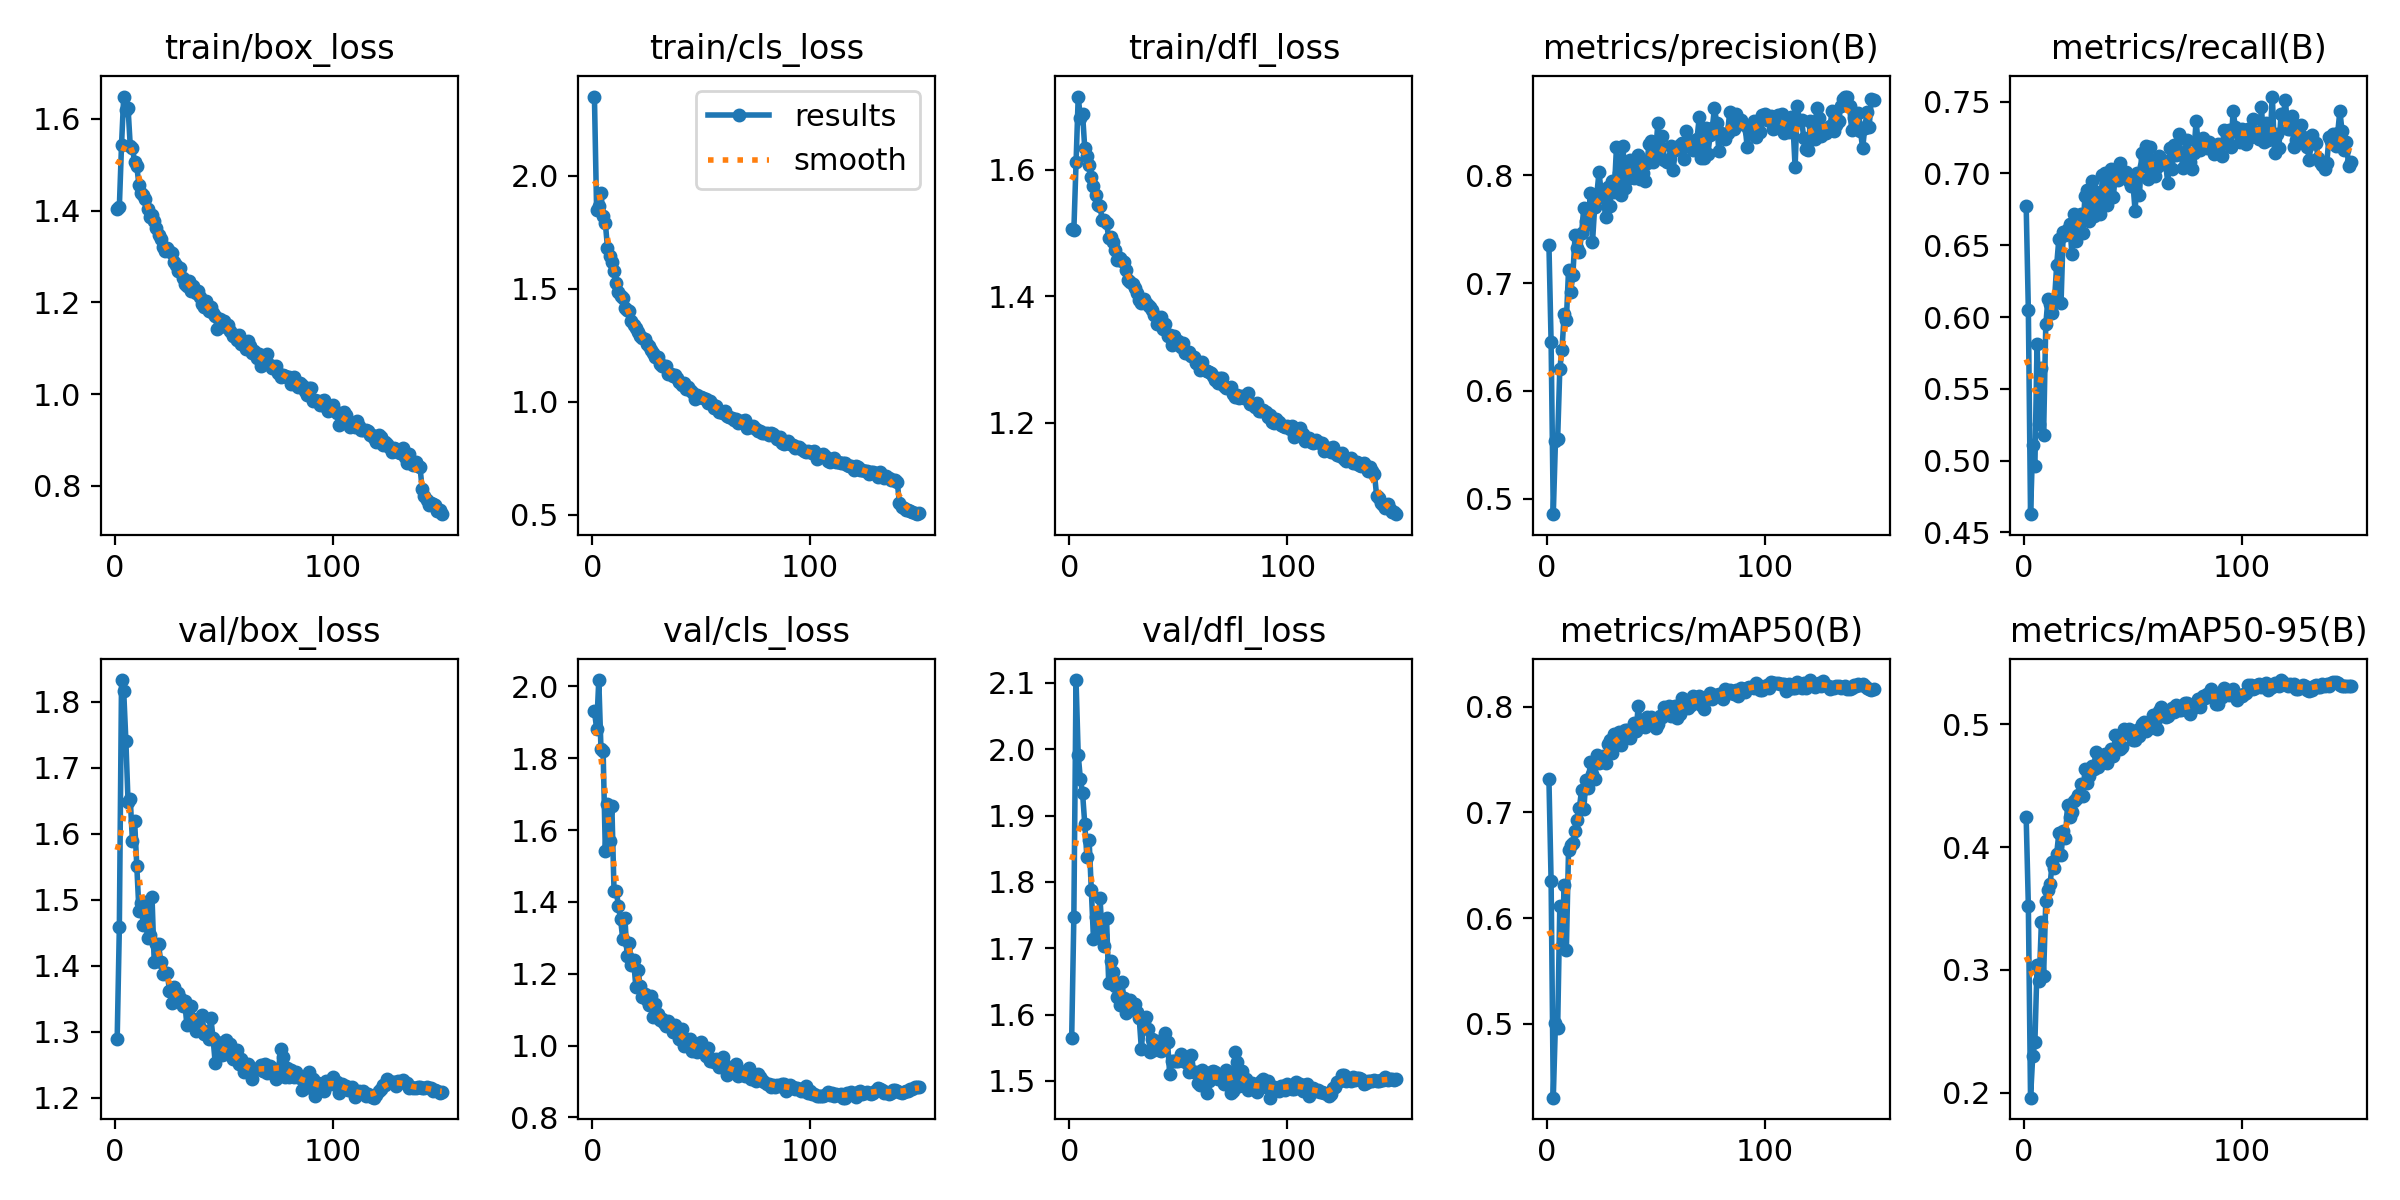
\includegraphics[scale=0.4]{gambar/loss 150 epoch.png}
    \caption{Visualisasi Hasil training}
    \label{fig:visualisasi hasil training}
\end{figure}


\begin{figure}[H]
    \centering
    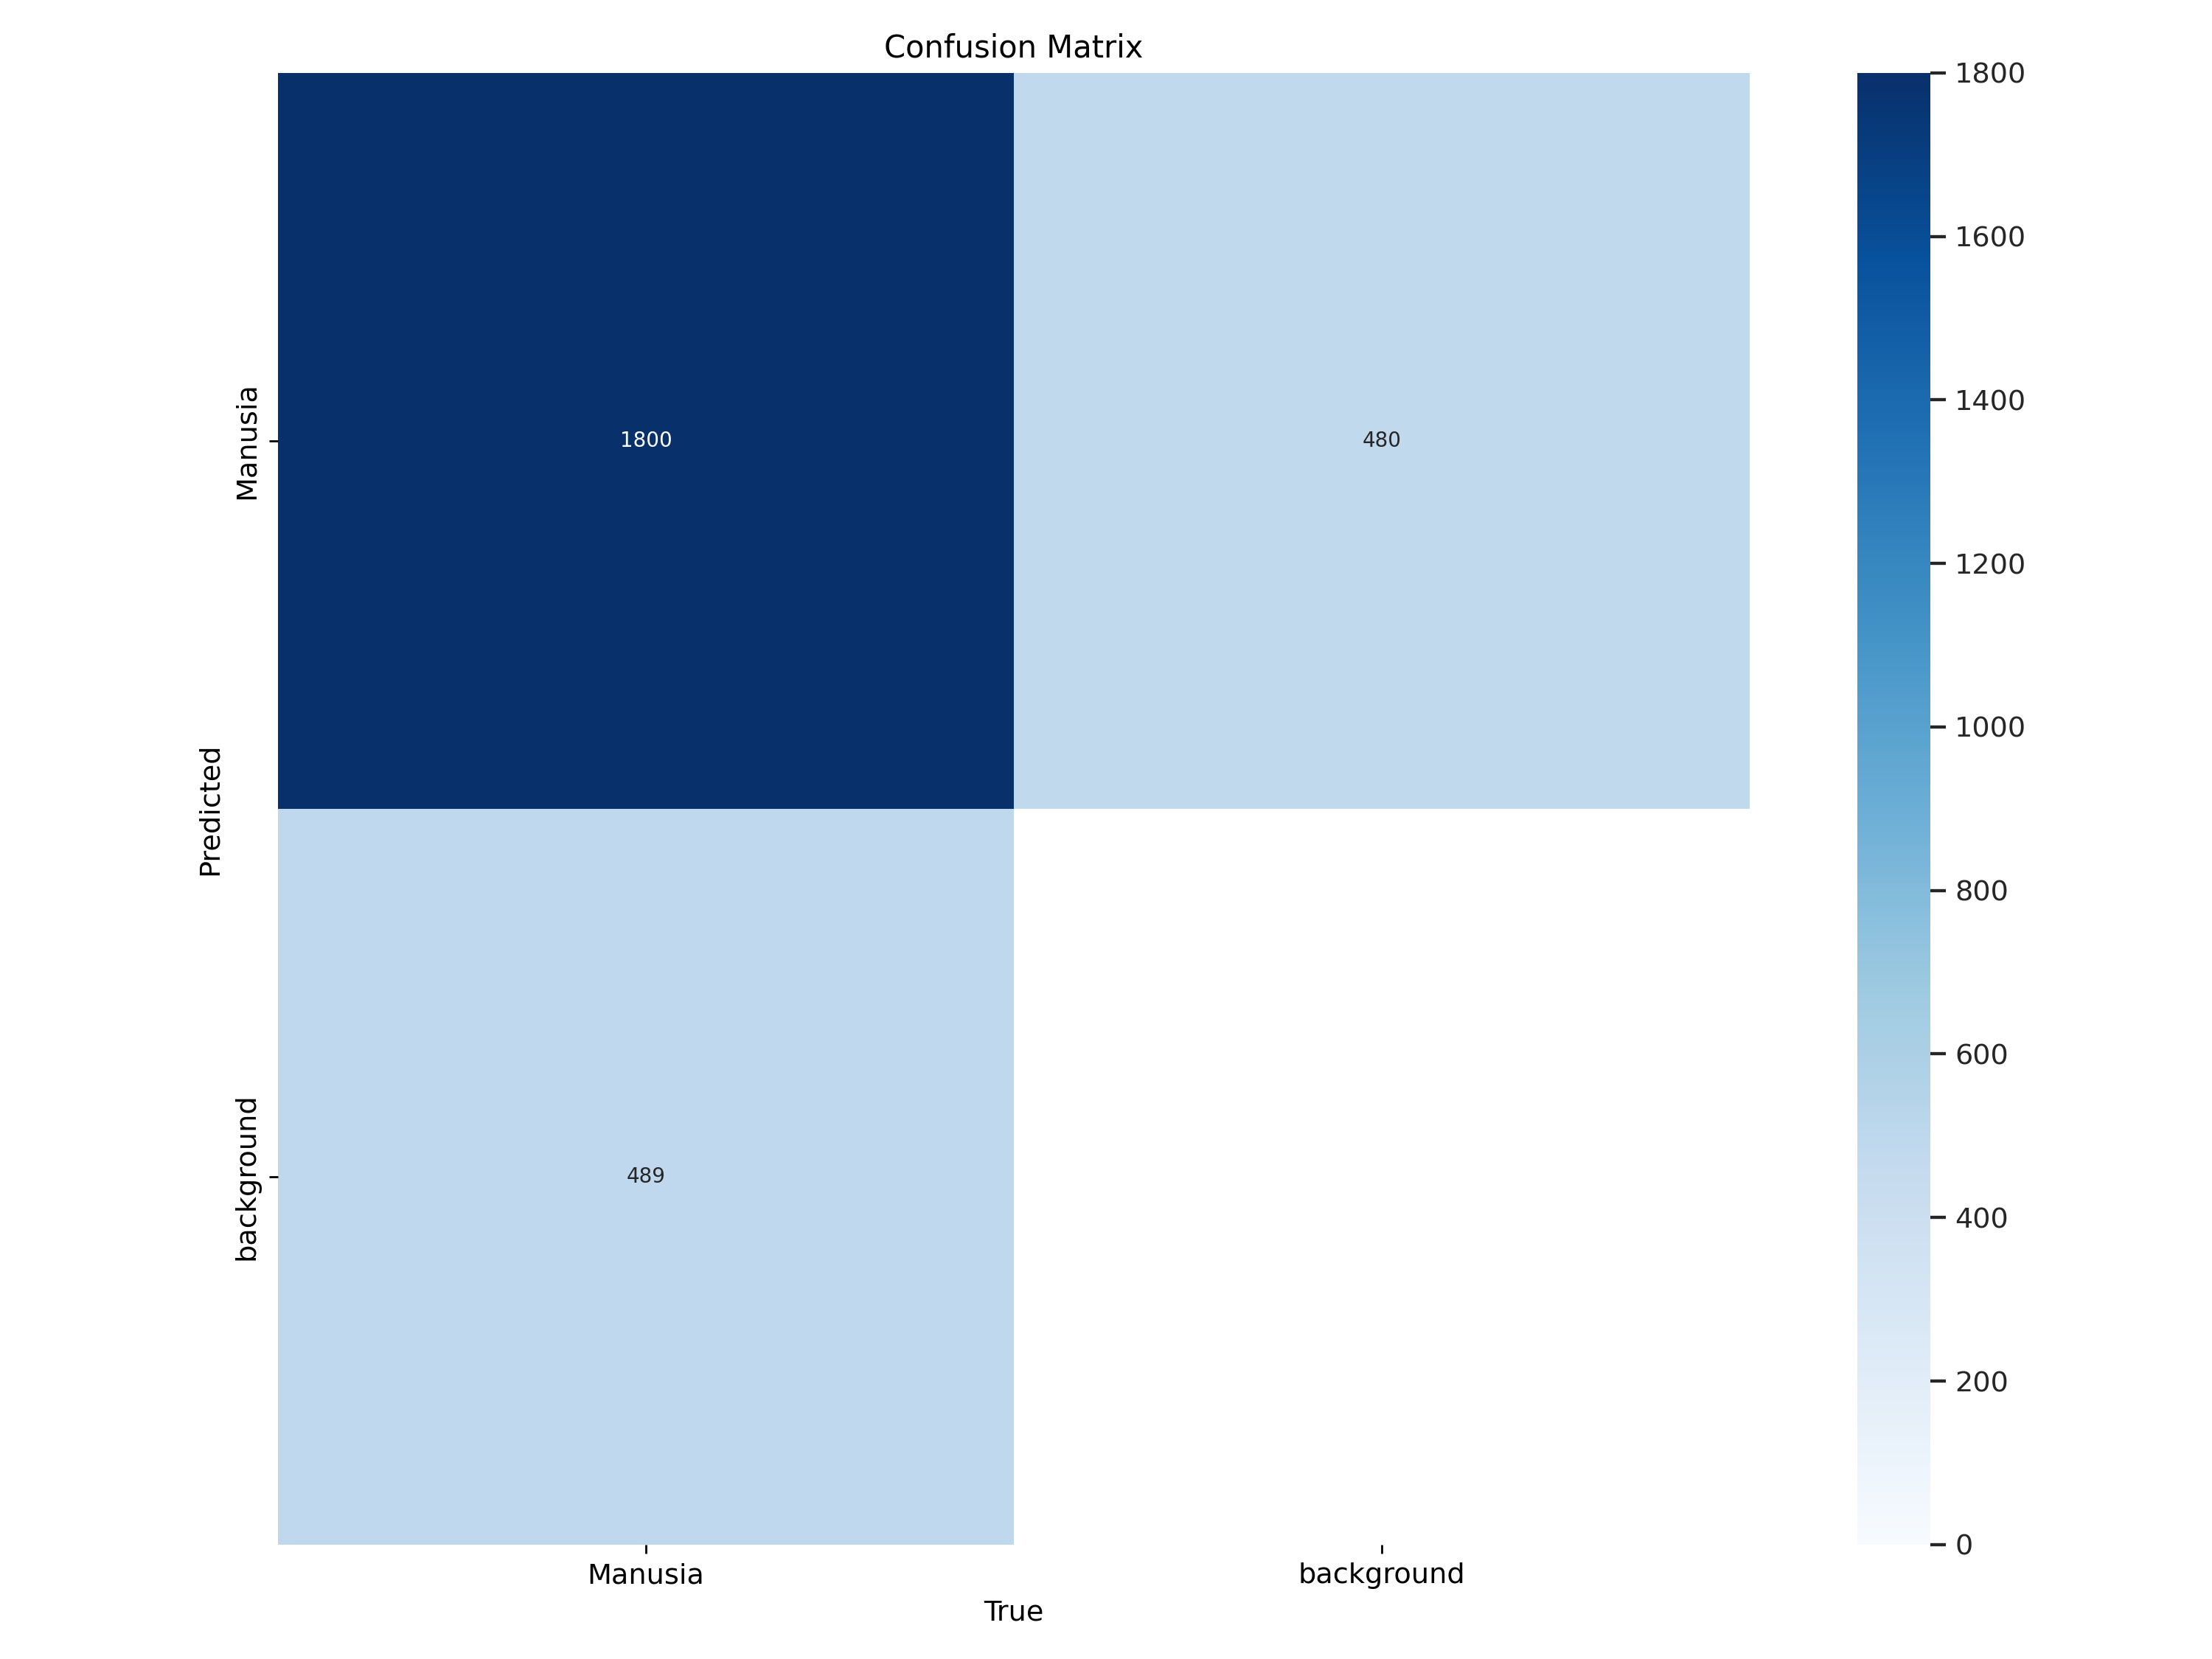
\includegraphics[scale=0.4]{gambar/confusion 150 epoch.png}
    \caption{Confusion Matrix Hasil Training}
    \label{fig:visualisasi hasil training}
\end{figure}

Dapat dilihat pada dapat dilihat bahwa dari hasil klasifikasi model terdapat 1800 data citra yang termasuk dalam kategori true positive, 480 citra yang termasuk dalam kategori false positive dan 489 citra yang termasuk false negative.

Dilakukan pula tes inference model yang telah dilatih menggunakan set data test terhadap object manusia. Dapat dilihat pada gambar dibawah nilai confidence score yang cukup tinggi.

\begin{figure}[H]
    \centering
    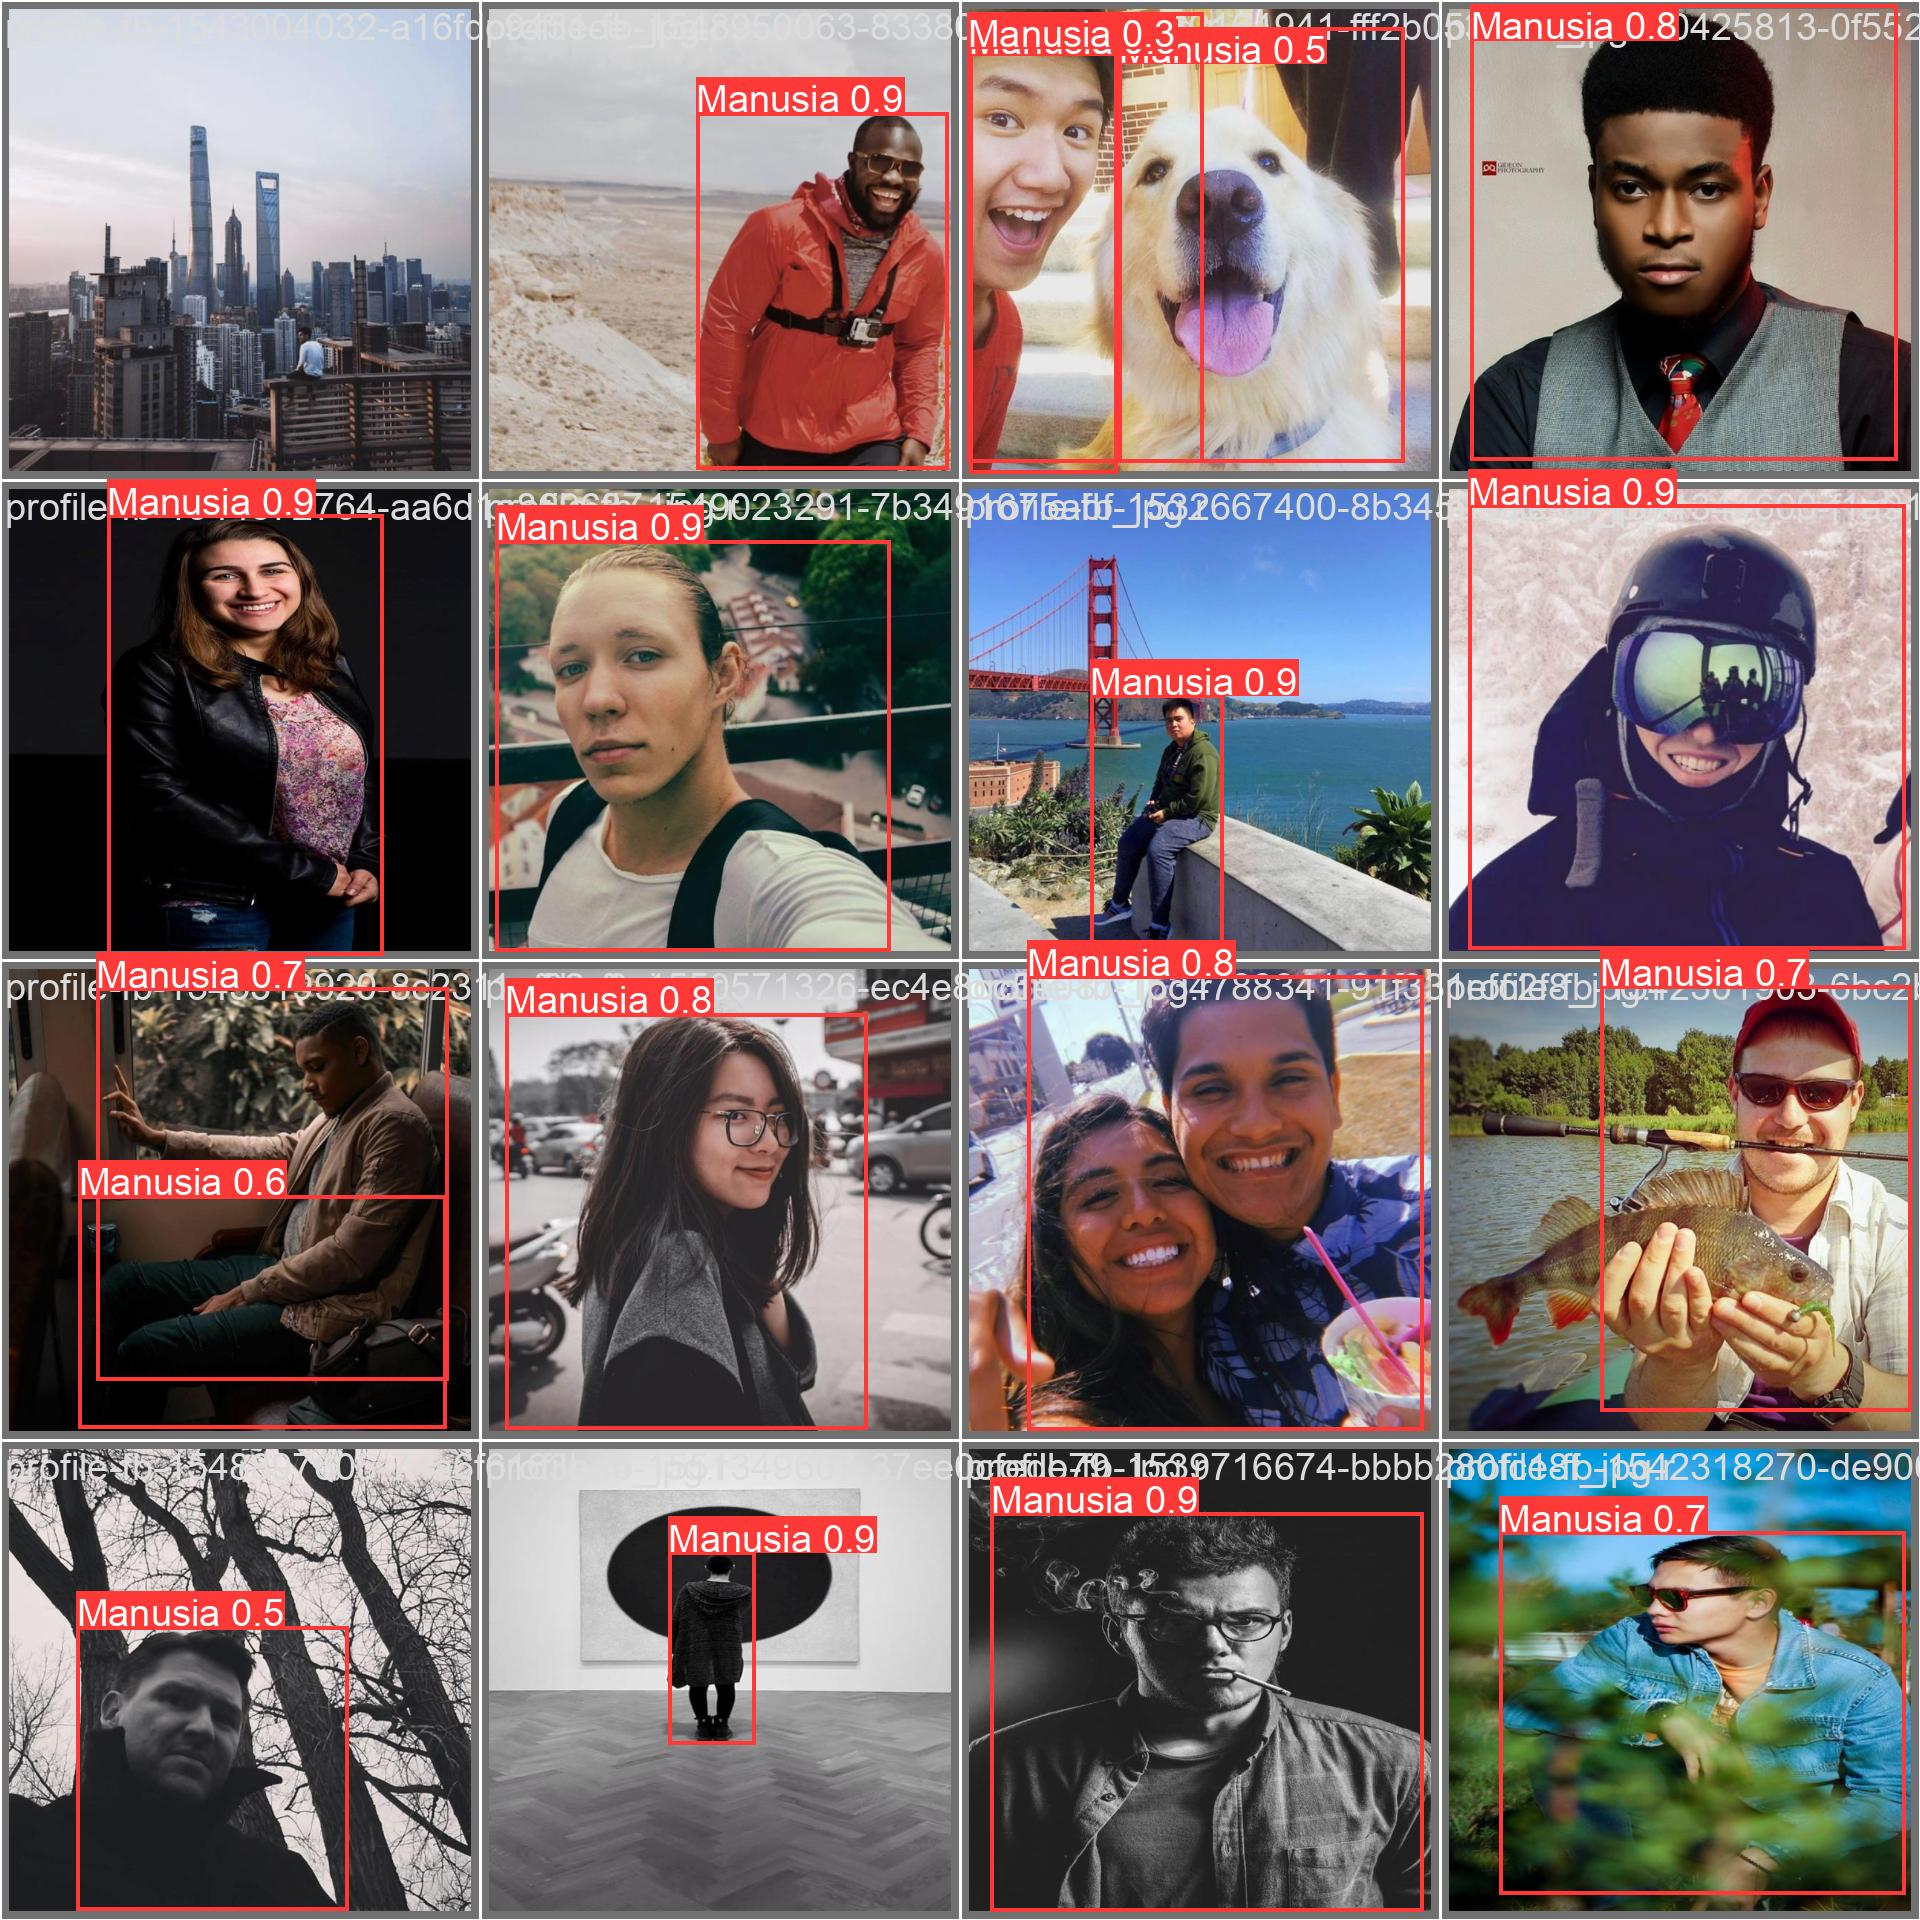
\includegraphics[scale=0.1]{gambar/confiden 150 epoch.jpg}
    \caption{Tes Inferensi Menggunakan Model Terlatih}
    \label{fig:visualisasi hasil training}
\end{figure}

\begin{figure}[H]
    \centering
    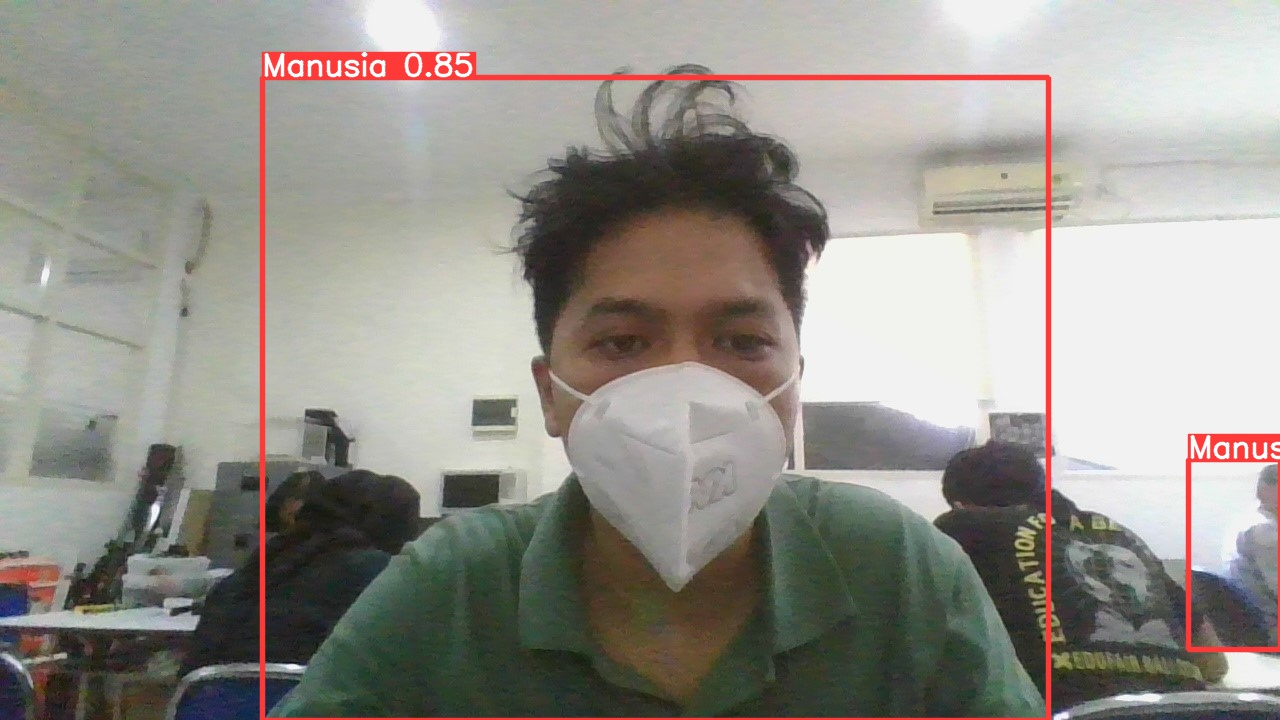
\includegraphics[scale=0.2]{gambar/confiden foto agung 150 epoch.jpg}
    \caption{Tes Inferensi Menggunakan Model Terlatih}
    \label{fig:enter-label}
\end{figure}

\subsubsection*{Perbandingan Evaluasi}

Dari kedua hasil training tersebut akan diambil yang terbaik berdasarkan pertimbangan akurasi. Dimana hasil dari confusion matrix kedua training menunjukan hasil yang baik, untuk lebih memahami kemampuan dari model maka perlu dihitung menggunakan rumus evaluasi sebagai berikut :

\begin{equation}
    Accuracy = \frac{TP + TN}{TP + TN + FP + FN}
\end{equation}

Sehingga dengan menginput masing nilai confusion matrix sebagai berikut :

\begin{lstlisting}[language=Python]
# Asumsi FP dan TN 0 Karena tidak ada nilai prediksi lain kecuali kelas manusia
TP_100 = 1806
FN_100 = 483
TP_150 = 1800
FN_150 = 489
FP_150_assumed = 0
FP_100_assumed = 0

accuracy_150_assumed = TP_150 / (TP_150 + FN_150 + FP_150_assumed)
accuracy_100_assumed = TP_100 / (TP_100 + FN_100 + FP_100_assumed)

accuracy_150_assumed, accuracy_100_assumed
\end{lstlisting}

Dari hasil perhitungan diatas didapatkan nilai akurasi untuk masing training dengan epoch 100 dan 150 yaitu sebesar 78.90\% dan 78.64\%. Dari 2 nilai tersebut didapatkan indikasi bahwa mengurangi jumlah epoch tidak berpengaruh signifikan terhadap kemampuan model untuk mengenali manusia dengan benar, dan bahkan sedikit lebih efisien dalam hal ini. Ini bisa berguna untuk menghemat waktu dan sumber daya komputasi tanpa mengorbankan performa yang banyak. Sehingga dalam proses selanjutnya model dengan 100 epoch akan digunakan dalam melakukan pengujian pada NUC.




\section{Deployment Pada Hardware}
Proses Deployment yang dilakukan Pada bagian ini berupa evaluasi kinerja model yang diimplementasikan pada perangkat keras. Skenario untuk mengumpulkan data untuk pengujian dengan menggunakan kamera Logitech C920 yang dipasangkan pada kursi roda otonom untuk mendeteksi manusia. Pengujian kinerja deployment dilakukan terhadap model yang dihasilkan pada pelatahin dengan 100 epoch. Dimana implementasi ini untuk mengukur:
\begin{enumerate} 
    \item Performa FPS sistem deteksi pada NUC.
    \item Inference dan Response time pada sistem.
    \item Tingkat keberhasilan kursi roda otonom dalam menghindari manusia.
\end{enumerate}

\subsection{Performa Model Pada Intel NUC}
Berikut hasil deployment yang dilakukan pada Intel NUC. Instalasi model pada NUC menggunakan venv yang tersedia pada Visual Studio code ide. Instalasi library perlu dilakukan untuk menjalankan model pada Intel NUC. Model output model berupa perintah yang dikirimkan untuk menggerakan motor akan dicatat melalui perbandingan hasil pada terminal visual studio code dan pada Ardruino ide. Berikut merupakan contoh data mentah yang dihasilkan dari output deteksi : 

\begin{lstlisting}[language = python]
0: 480x800 1 Manusia, 102.8ms
Waktu respons MediaPipe: 0.03261 detik
FPS: 6.08
Manusia di kiri
Speed: 5.7ms preprocess, 102.8ms inference, 0.0ms postprocess per image at shape (1, 3, 480, 800)
Waktu respons YOLO: 0.000467 detik
\end{lstlisting}

Dapat dilihat nilai yang ditampilkan berupa Waktu response mediapipe, FPS dari sistem, posisi manusia , kecepatan preprocess, waktu inference pada sistem NUC, postprocess, dan waktu response YOLO.

Agar kita dapat dengan mudah membaca nilainya maka akan dilakukan proses olah data menggunakan python. Berikut merupakan teknik pengolahan data menjadi format CSV sebagai berikut:

\begin{lstlisting}[language = python]
import pandas as pd
import re

raw_data = """
0: 480x800 1 Manusia, 95.6ms
Waktu respons MediaPipe: 0.02218 detik
Jarak : 1.34
FPS: 6.37
Manusia di tengah
Speed: 5.2ms preprocess, 95.6ms inference, 0.0ms postprocess per image at shape (1, 3, 480, 800)
Waktu respons YOLO: 0.00047 detik
"""

def parse_data_block(block):
    lines = block.strip().split('\n')
    parsed_data = {
        'Inference': float(re.findall(r"(\d+\.\d+)ms", lines[0])[0]),
        'MediaPipe Response Time': float(re.findall(r"(\d+\.\d+) detik", lines[1])[0]),
        'Jarak': float(re.findall(r"Jarak : (\d+\.\d+)", lines[2])[0]),
        'FPS': float(re.findall(r"FPS: (\d+\.\d+)", lines[3])[0]),
        'Position': lines[4],
        'Preprocess Time': float(re.findall(r"(\d+\.\d+)ms preprocess", lines[5])[0]),
        'Postprocess Time': float(re.findall(r"(\d+\.\d+)ms postprocess", lines[5])[0]),
        'YOLO Response Time': float(re.findall(r"(\d+\.\d+) detik", lines[6])[0])
    }
    return parsed_data

blocks = raw_data.strip().split('\n\n')
data = [parse_data_block(block) for block in blocks]

df = pd.DataFrame(data)

csv_path = "/mnt/data/processed_data_v2.csv"
df.to_csv(csv_path, index=False)

csv_path, df.head()
\end{lstlisting}

Dengan menjalankan program tersebut akan didapatkan tabel yang berisikan Waktu response mediapipe, FPS dari sistem, posisi manusia , kecepatan preprocess, waktu inference pada sistem NUC, postprocess, dan waktu response YOLO. Nilai - nilai yang didapatkan dari program tersebut akan dilakukan pengujian pada bagian selanjutnya dan diambil kesimpulan.  

\subsection{Pengujian Berdasarkan FPS}
Pengujian FPS akan dilakukan pada dua device yang pertama adalah pengujian pada device Laptop, dan pengujian pada device NUC. Dalam pengujian ini akan diambil nilai FPS sesuai dengan output yang didapatkan dan sudah diolah pada bagian sebelumnya.

\subsubsection{1. Pengujian pada Laptop}
Pada pengujian ini akan diambil nilai FPS pada laptop. Spesifikasi laptop yang digunakan pada pengujian ini merupakan sebagai berikut :

\begin{longtable}{|c|c|}
  \caption{Spesifikasi Laptop}
  \label{tb:Spesifikasi Laptop}                                   \\
  \hline
  \rowcolor[HTML]{C0C0C0}
  \textbf{Komponen} & \textbf{Spesifikasi}  \\
  \hline
  CPU            & Intel(R) Core(TM) i5-10300H CPU @2.50GHz(8CPU)        \\
  RAM            & 16 GB DDR4-2666 SDRAM        \\
  GPU            & NVIDIA® GeForce RTX™ 2060 with Max-Q design           \\
  \hline
\end{longtable}
Dapat dilihat pada tabel dibawah, didapatkan pada pengujian ini nilai rata - rata FPS sebesar 13.140. Dimana nilai FPS tertinggi adalah sebesar 13.23 dan FPS paling rendah ialah 13.05. Kestabilan nilai pada Pengujian ini menandakan bahwa performa sistem yang dijalankan pada laptop berjalan dengan sangat baik dan efisien.
\begin{table}[H]
    \centering
    \caption{Tabel FPS pada Laptop}
    \label{tb:FPS pada Laptop}                          \\
    \begin{tabular}{|l|l|}
    \hline
        No & FPS \\ \hline
        1 & 13.23 \\ \hline
        2 & 13.23 \\ \hline
        3 & 13.23 \\ \hline
        4 & 13.23 \\ \hline
        5 & 13.23 \\ \hline
        6 & 13.23 \\ \hline
        7 & 13.23 \\ \hline
        8 & 13.23 \\ \hline
        9 & 13.23 \\ \hline
        10 & 13.23 \\ \hline
        11 & 13.23 \\ \hline
        12 & 13.23 \\ \hline
        13 & 13.23 \\ \hline
        14 & 13.23 \\ \hline
        15 & 13.05 \\ \hline
        16 & 13.05 \\ \hline
        17 & 13.05 \\ \hline
        18 & 13.05 \\ \hline
        19 & 13.05 \\ \hline
        20 & 13.05 \\ \hline
        21 & 13.05 \\ \hline
        22 & 13.05 \\ \hline
        23 & 13.05 \\ \hline
        24 & 13.05 \\ \hline
        25 & 13.05 \\ \hline
        26 & 13.05 \\ \hline
        27 & 13.05 \\ \hline
        28 & 13.05 \\ \hline
        29 & 13.05 \\ \hline
        30 & 13.05 \\ \hline
    \end{tabular}
\end{table} 

\subsubsection*{2. Pengujian pada NUC}
Pada pengujian ini akan diambil nilai FPS pada NUC. Spesifikasi NUC yang digunakan pada pengujian ini merupakan sebagai berikut :

\begin{longtable}{|c|c|}
    \caption{Spesifikasi NUC}
    \label{tb:Spesifikasi NUC}                             \\
    \hline   
    \rowcolor[HTML]{C0C0C0}
    \textbf{Komponen} & \textbf{Spesifikasi} \\
    \hline
  CPU            &  Intel® Core™ i7-1165G7        \\
  RAM            & 32 GBLPDDR4        \\
  OS            & Windows 11 Home Single Language           \\
\end{longtable}
Dapat dilihat pada tabel dibawah, didapatkan pada pengujian ini nilai rata - rata FPS sebesar 6.111. Dimana nilai FPS tertinggi yang didapatkan ialah 6.47 dan FPS paling rendah ialah 5.54. Performa yang dihasilkan pada NUC tergolong stabil namun hasilnya kurang mendekati performa laptop.

\begin{table}[H]
    \centering
    \caption{Tabel FPS pada NUC}
    \label{tb:TabelFPS}                                        \\
    \begin{tabular}{|l|l|}
    \hline
        No & FPS \\ \hline
        1 & 6.37 \\ \hline
        2 & 6.43 \\ \hline
        3 & 6.43 \\ \hline
        4 & 5.57 \\ \hline
        5 & 5.54 \\ \hline
        6 & 5.79 \\ \hline
        7 & 5.83 \\ \hline
        8 & 6.42 \\ \hline
        9 & 6.47 \\ \hline
        10 & 6.47 \\ \hline
        11 & 6.47 \\ \hline
        12 & 6.42 \\ \hline
        13 & 6.42 \\ \hline
        14 & 6.42 \\ \hline
        15 & 6.42 \\ \hline
        16 & 6.43 \\ \hline
        17 & 6.42 \\ \hline
        18 & 6.42 \\ \hline
        19 & 6.47 \\ \hline
        20 & 6.42 \\ \hline
        21 & 6.42 \\ \hline
        22 & 6.43 \\ \hline
        23 & 6.42 \\ \hline
        24 & 6.42 \\ \hline
        25 & 6.47 \\ \hline
        26 & 6.42 \\ \hline
        27 & 6.42 \\ \hline
        28 & 6.37 \\ \hline
        29 & 6.43 \\ \hline
        30 & 6.33 \\ \hline
    \end{tabular}
\end{table}
 
\subsection{Pengujian Berdasarkan Hasil Response Time}
Untuk dapat melakukan pengujian hasil response time, maka obstacle harus memenuhi syarat Near Object Condition yang telah dibahas pada bab sebelumnya. Output yang dihasilkan setiap kali penghindaran berisi Arah dan time stamp pada Ardruino IDE dan Visual Studio code. Berikut merupakan contoh data mentah untuk kedua hasil output: 

\begin{lstlisting}[language=c]
22:18:32.273 -> Stop
22:18:32.948 -> Arah : E
22:18:33.131 -> Kanan
22:18:33.759 -> Arah : C
22:18:33.936 -> Stop
22:18:34.748 -> Arah : B
22:18:35.121 -> Maju
22:18:35.439 -> Arah : C
22:18:35.815 -> Stop
22:18:36.410 -> Arah : E
22:18:36.616 -> Kanan
\end{lstlisting}


Output yang didapatkan pada ardruino berisikan Timestamp. Timestamp yang dihasilkan yaitu \emph{Timestamp Receive ESP} dan \emph{Timestamp Receive Motor}. Selain pada ardruino pada vscode juga didapatkan nilai time stamp \emph{sent}, contoh outputnya dapat dilihat sebagai berikut.

\begin{lstlisting}[language=python]
BELOK KANAN,0.8,2024-05-08 22:18:14.263
MAJU,0.4,2024-05-08 22:18:18.762
BELOK KANAN,0.0,2024-05-08 22:18:28.614
MAJU,0.0,2024-05-08 22:18:30.940
BELOK KANAN,1.2,2024-05-08 22:18:32.899
MAJU,0.8,2024-05-08 22:18:34.728
BELOK KANAN,0.0,2024-05-08 22:18:36.392
\end{lstlisting}

Berdasarkan output diatas dapat dihitung Response Time sistem yang akan jabarkan pada tabel selanjutnya Hasil Response Time akan diuji untuk mendapatkan waktu yang dibutuhkan untuk melakukan pendeteksian dengan model yang kemudian diklasifikasi dan dikirim ke ESP32 hingga mo tor kursi roda mulai bergerak. Pengujian ini dilakukan secara real time pada perangkat NUC, perhitungan delay didapatkan dari mulai dikirim hingga berhentinya motor pada kursi roda. sedangkan perhitungan inference time dimulai dari dimulainya proses prediksi hingga didapatkan hasil dari proses klasifikasi. Rata - rata waktu delay yang didapatkan adalah 0.248 dari data yang sudah didapatkan dari pengujian NUC, adapun hasil nya dapat dilihat pada tabel dibawah. Adapun nilai inference rata-rata yang didapatkan adalah 
\begin{table}[H]
    \caption{Hasil Pengujian Response Time}
    \centering
    \begin{tabular}{|l|l|l|l|l|l|}
    \hline
        Inference & Sent & Receive & Motor & Delay & Arah \\ \hline
        125.0 & 19:53:02.763 & 19:53:02.800 & 19:53:03.178 & 0.378 & Stop \\ \hline
        131.5 & 19:53:06.543 & 19:53:06.572 & 19:53:06.760 & 0.188 & Maju \\ \hline
        139.5 & 19:53:08.800 & 19:53:08.826 & 19:53:09.014 & 0.188 & Stop \\ \hline
        154.1 & 19:53:14.058 & 19:53:14.118 & 19:53:14.450 & 0.262 & Kanan \\ \hline
        131.6 & 19:53:17.932 & 19:53:17.974 & 19:53:18.162 & 0.188 & Stop \\ \hline
        141.9 & 19:53:19.645 & 19:53:19.667 & 19:53:19.855 & 0.188 & Kiri \\ \hline
        136.7 & 19:53:29.266 & 19:53:29.287 & 19:53:29.477 & 0.190 & Stop \\ \hline
        132.7 & 19:53:35.816 & 19:53:35.854 & 19:53:36.230 & 0.376 & Maju \\ \hline
        152.5 & 19:53:42.816 & 19:53:42.868 & 19:53:43.059 & 0.191 & Stop \\ \hline
        136.5 & 19:53:46.210 & 19:53:46.249 & 19:53:46.437 & 0.188 & Kiri \\ \hline
        141.8 & 19:53:55.093 & 19:53:55.124 & 19:53:55.314 & 0.190 & Stop \\ \hline
        140.1 & 19:54:01.549 & 19:54:01.586 & 19:54:01.766 & 0.180 & Kanan \\ \hline
        127.5 & 19:54:03.265 & 19:54:03.319 & 19:54:03.509 & 0.190 & Stop \\ \hline
        135.5 & 19:54:04.964 & 19:54:05.010 & 19:54:05.373 & 0.363 & Kiri \\ \hline
        142.5 & 19:54:20.862 & 19:54:20.886 & 19:54:21.073 & 0.187 & Stop \\ \hline
        136.6 & 19:54:22.398 & 19:54:22.440 & 19:54:22.819 & 0.379 & Maju \\ \hline
        123.1 & 19:54:24.094 & 19:54:24.133 & 19:54:24.323 & 0.190 & Stop \\ \hline
        143.4 & 19:54:32.486 & 19:54:32.517 & 19:54:32.713 & 0.196 & Kiri \\ \hline
        141.6 & 19:54:34.426 & 19:54:34.492 & 19:54:34.871 & 0.379 & Stop \\ \hline
        129.6 & 19:54:36.177 & 19:54:36.231 & 19:54:36.376 & 0.145 & Kanan \\ \hline
        152.1 & 19:54:37.870 & 19:54:37.923 & 19:54:38.111 & 0.188 & Stop \\ \hline
        134.2 & 19:54:40.144 & 19:54:40.177 & 19:54:40.546 & 0.369 & Kiri \\ \hline
        136.4 & 19:54:42.220 & 19:54:42.234 & 19:54:42.422 & 0.188 & Stop \\ \hline
        133.5 & 19:54:43.909 & 19:54:43.926 & 19:54:44.289 & 0.363 & Kanan \\ \hline
        137.1 & 19:54:51.301 & 19:54:51.333 & 19:54:51.523 & 0.190 & Stop \\ \hline
        140.1 & 19:54:54.763 & 19:54:54.796 & 19:54:55.142 & 0.346 & Kiri \\ \hline
        135.5 & 19:54:56.502 & 19:54:56.551 & 19:54:56.742 & 0.191 & Stop \\ \hline
        181.1 & 19:54:58.584 & 19:54:58.619 & 19:54:58.981 & 0.362 & Maju \\ \hline
        141.5 & 19:55:00.444 & 19:55:00.487 & 19:55:00.678 & 0.191 & Stop \\ \hline
        149.5 & 19:55:05.502 & 19:55:05.576 & 19:55:05.936 & 0.360 & Kanan \\ \hline
    \end{tabular}
\end{table}

\subsection{Performa Keberhasilan}
Pengujian ini dilakukan pengetesan terhadap kursi roda dalam menghindari Manusia secara real time. Pengetesan ini akan dilakukan Pada Tower 2 ITS. Pada pengujian ini diambil 20 kali sampel dan dicatat keberhasilan penghindaran. Manusia yang dideteksi Diam dan tidak bergerak. Hasil yang didapatkan sebagai berikut 

\begin{table}[H]
\centering
\begin{tabular}{|l|l|}
\hline
Percobaan Ke & Hasil                                                               \\ \hline
1            & \cellcolor[HTML]{67FD9A}Kursi Roda Berhasil Menghindar              \\ \hline
2            & \cellcolor[HTML]{67FD9A}Kursi Roda Berhasil Menghindar              \\ \hline
3            & \cellcolor[HTML]{67FD9A}Kursi Roda Berhasil Menghindar              \\ \hline
4            & \cellcolor[HTML]{67FD9A}Kursi Roda Berhasil Menghindar              \\ \hline
5            & \cellcolor[HTML]{67FD9A}Kursi Roda Berhasil Menghindar              \\ \hline
6            & \cellcolor[HTML]{67FD9A}Kursi Roda Berhasil Menghindar              \\ \hline
7            & \cellcolor[HTML]{67FD9A}Kursi Roda Berhasil Menghindar              \\ \hline
8            & \cellcolor[HTML]{67FD9A}Kursi Roda Berhasil Menghindar              \\ \hline
9            & \cellcolor[HTML]{67FD9A}Kursi Roda Berhasil Menghindar              \\ \hline
10           & \cellcolor[HTML]{67FD9A}Kursi Roda Berhasil Menghindar              \\ \hline
11           & \cellcolor[HTML]{FD6864}Objek tidak terdeteksi dan Gagal Menghindar \\ \hline
12           & \cellcolor[HTML]{67FD9A}Kursi Roda Berhasil Menghindar              \\ \hline
13           & \cellcolor[HTML]{67FD9A}Kursi Roda Berhasil Menghindar              \\ \hline
14           & \cellcolor[HTML]{67FD9A}Kursi Roda Berhasil Menghindar              \\ \hline
15           & \cellcolor[HTML]{67FD9A}Kursi Roda Berhasil Menghindar              \\ \hline
16           & \cellcolor[HTML]{67FD9A}Kursi Roda Berhasil Menghindar              \\ \hline
17           & \cellcolor[HTML]{67FD9A}Kursi Roda Berhasil Menghindar              \\ \hline
18           & \cellcolor[HTML]{67FD9A}Kursi Roda Berhasil Menghindar              \\ \hline
19           & \cellcolor[HTML]{67FD9A}Kursi Roda Berhasil Menghindar              \\ \hline
20           & \cellcolor[HTML]{67FD9A}Kursi Roda Berhasil Menghindar              \\ \hline
\end{tabular}
\end{table}

Berdasarkan Hasil yang didapatkan Penghindaran berhasil sebanyak 19 kali dan gagal 1 kali pada percobaan ke 11. Adapun presentasi yang didapatkan dari hasil uji ini sebesar 98\%
\cleardoublepage

% Bab 5 penutup
\chapter{PENUTUP}
\label{chap:penutup}

% Ubah bagian-bagian berikut dengan isi dari penutup

\section{Kesimpulan}
\label{sec:kesimpulan}

Berdasarkan hasil pengujian yang telah dilakukan, dapat ditarik kesimpulan sebagai berikut:

\begin{enumerate}[nolistsep]
  \item Model dengan Metrics tertinggi yang telah di-training dengan berbagai konfigurasi dan arsitektur adalah model dengan skor mAP di IoU 0.5 tertinggi sebesar 94.10\% yang menggunakan arsitektur SSD-Mobilenet-V2 FPN-Lite 320, skor tersebut lebih tinggi dibandingkan penelitian sebelumnya yang digunakan sebagai referensi
  \item Performa NUC dalam pengujian FPS menghasilkan Nilai yang lebih rendah ketimbang Laptop pribadi Penulis dengan selisih 7.029
  \item Rata - rata delay yang didapatkan pada pengujian adalah sekitar 0.248 dan rata- rata nilai inference yang didapatkan
  \item Hasil Performa Deteksi menunjukan hasil yang memuaskan dalam 10 sampel pengujian. Dengan presentasi keberhasilan sebesar 100\%

\end{enumerate}

\section{Saran}
\label{chap:saran}

Untuk pengembangan lebih lanjut pada penelitian selanjutnya, adapun saran yang bisa diberikan antara lain:

\begin{enumerate}[nolistsep]

  \item Variasi dataset yang lebih ditingkat untuk meningkatkan performa deteksi

  \item Menggunakan SBC yang memiliki performa yang lebih baik untuk fps yang lebih tinggi

  \item Meningkatkan performa grid dengan mengubah ukuran 10x10 menjadi 100x100 atau lebih untuk hasil lebih detail

\end{enumerate}

\cleardoublepage

\chapter*{DAFTAR PUSTAKA}
\addcontentsline{toc}{chapter}{DAFTAR PUSTAKA}
\renewcommand\refname{}
\vspace{2ex}
\renewcommand{\bibname}{}
\begingroup
\def\chapter*#1{}
\printbibliography
\endgroup
\cleardoublepage

\chapter*{LAMPIRAN}

\section*{Kode Program}
\subsection*{Sistem Penghindaran Menggunakan YoloV8}
% Program 3.1 
\begin{lstlisting}[language=Python]
from ultralytics import YOLO
import cv2
import math
import mediapipe as mp
import numpy as np
import socket
import time
import datetime
from mediapipe.python.solutions.pose import PoseLandmark

def delay(seconds):
    start_time = time.time()
    while time.time() - start_time < seconds:
        pass

host = "192.168.4.1" # Set to ESP32 Access Point IP Address
port = 80

mp_pose = mp.solutions.pose
pose = mp_pose.Pose(static_image_mode=False, min_detection_confidence=0.6)
mp_drawing = mp.solutions.drawing_utils


cap = cv2.VideoCapture(0)
cap.set(3, 1920)  
cap.set(4, 1080)  

k = 10.311 
k2 = 24.222

focal_length_pixel = 481  
tinggi_objek_nyata = 181  


frame_count = 0
start_time = time.time()
fps = 0

model = YOLO("best2.pt")

def hitung_jarak(tinggi_bounding_box, focal_length_pixel, tinggi_objek_nyata):
    if tinggi_bounding_box == 0:
        return float('inf') 
    jarak = (tinggi_objek_nyata * focal_length_pixel) / tinggi_bounding_box
    return jarak / 100  # Konversi ke meter

def hitung_lebar_objek(lebar_bounding_box, jarak_objek, focal_length_pixel):
    if lebar_bounding_box == 0 or focal_length_pixel == 0:
        return 0 
    lebar_objek = (lebar_bounding_box * jarak_objek) / focal_length_pixel
    return lebar_objek

def convert_coordinates(outputs, img_width, img_height):
    boxes = []
    for detection in outputs:
        x_center, y_center, width, height = detection['x_center'], detection['y_center'], detection['width'], detection['height']
        
        x_min = (x_center - width / 2) * img_width
        y_min = (y_center - height / 2) * img_height
        x_max = (x_center + width / 2) * img_width
        y_max = (y_center + height / 2) * img_height
        
        boxes.append((x_min, y_min, x_max, y_max))
    return boxes

# Fungsi untuk menghitung jarak Euclidean dalam piksel
def hitung_jarak_euclidean(landmark1, landmark2, lebar_img):
    jarak_pix = math.sqrt((landmark1.x - landmark2.x) ** 2 + (landmark1.y - landmark2.y) ** 2) * lebar_img
    return jarak_pix

def hitung_lebar_mediapipe(pose_results, lebar_img):
    if pose_results.pose_landmarks:
        bahu_kiri = pose_results.pose_landmarks.landmark[mp_pose.PoseLandmark.LEFT_SHOULDER]
        bahu_kanan = pose_results.pose_landmarks.landmark[mp_pose.PoseLandmark.RIGHT_SHOULDER]
        jarak_pix = hitung_jarak_euclidean(bahu_kiri, bahu_kanan, lebar_img)
        
        faktor_konversi = 0.00087  # 0.087cm per piksel
        lebar_m = jarak_pix * faktor_konversi
        
        return lebar_m
    return 0

def hitung_jarak_vertikal(pose_results, tinggi_img):
    if pose_results.pose_landmarks:
        pusar = pose_results.pose_landmarks.landmark[mp_pose.PoseLandmark.NOSE]
        # Misal kita asumsikan pusar sebagai acuan vertikal (bisa diganti sesuai dengan landmark yang sesuai)
        jarak_vertikal = (1 - pusar.y) * tinggi_img  # Hitung jarak dari atas gambar ke pusar
        return jarak_vertikal
    return 0

def draw_grid(img, detection_status, camera_position):
    grid_size = 100  # Ukuran grid di sudut kanan bawah
    start_x = img.shape[1] - grid_size - 10  # Posisi X grid
    start_y = img.shape[0] - grid_size - 10  # Posisi Y grid

    cell_size = int(grid_size / 10)  # Membagi grid menjadi 10x10

    # Menggambar sel grid dengan latar belakang putih
    for i in range(10):
        for j in range(10):
            cell_color = (255, 0, 0) if detection_status[i][j] else (0, 0, 0)
            cv2.rectangle(img, (start_x + j * cell_size, start_y + i * cell_size),
                          (start_x + (j + 1) * cell_size, start_y + (i + 1) * cell_size), cell_color, -1)

    # Menandai posisi kamera dengan kotak hijau
    for pos in camera_position:
        x, y = pos
        cv2.rectangle(img, (start_x + x * cell_size, start_y + y * cell_size),
                      (start_x + (x + 1) * cell_size, start_y + (y + 1) * cell_size), (0, 255, 0), -1)
        
    # Menggambar garis grid
    for i in range(11):
        cv2.line(img, (start_x, start_y + i * cell_size), (start_x + grid_size, start_y + i * cell_size), (255, 255, 255), 1)
        cv2.line(img, (start_x + i * cell_size, start_y), (start_x + i * cell_size, start_y + grid_size), (255, 255, 255), 1)
    
    text_x2 = start_x - 10
    text_x = start_x - 80
    text_y = start_y - 20  # Menempatkan teks 20 piksel di atas grid
    text_y2 = start_y - 80
    cv2.putText(img, "0.2 Meter per square", (text_x,text_y), cv2.FONT_HERSHEY_SCRIPT_SIMPLEX, 0.6, (255,255,255), 1)
    cv2.putText(img, f"X: {posisi_horizontal_piksel:.2f}px", (text_x2, text_y2), cv2.FONT_HERSHEY_SIMPLEX, 0.6, (255, 255, 255), 1)

    return img

def determine_direction(detection_grid, grid_size=10):
    mid_point = grid_size // 2
    left_count = np.sum(detection_grid[:, :mid_point])
    right_count = np.sum(detection_grid[:, mid_point:])
    manusia = None
    
    #if jarak_mediapipe <0.7:
    if left_count > right_count:
        direction = 'Kiri'
        manusia = "Manusia di Kanan"
    
    elif right_count > left_count:
        direction = 'Kanan'
        manusia = "Manusia di Kiri"
            
    else:
        direction = 'Kanan'
        manusia = "Manusia di tengah"
    #else:
    #    direction = (["Terus Maju"])

        
    return direction, abs(right_count - left_count) * 0.2, manusia  # Misalkan setiap kotak mewakili 0.2 meter


# Inisialisasi grid deteksi
detection_grid = np.zeros((10, 10), dtype=bool)
camera_position = [(4, 0), (5, 0)]  # Posisi kamera pada grid (5,10) dan (6,10)
newtex = None

while True:
    success, img = cap.read()
    if not success:
        break  # Jika tidak berhasil membaca frame, keluar dari loop

    frame_count += 1
    current_time = time.time()

    # Hitung dan tampilkan FPS setiap satu detik
    if current_time - start_time >= 1:
        fps = frame_count / (current_time - start_time)
        frame_count = 0
        start_time = current_time
        print(f"FPS: {fps:.2f}")

    detection_grid.fill(False)
    detection_grid[0, 4] = True  # Pos 5,10 dalam 0-index
    detection_grid[0, 5] = True  # Pos 6,10 dalam 0-index
    img = cv2.cvtColor(img, cv2.COLOR_BGR2RGB)

    start_time_yolo = time.time()

    results = model.predict(img, stream=True)

    end_time_yolo = time.time()

    response_time_yolo = end_time_yolo - start_time_yolo
    print(f"Waktu respons YOLO: {response_time_yolo:.5f} detik")

#print waktu
    for r in results:
        boxes = r.boxes

        for box in boxes:
            confidence = math.ceil((box.conf[0] * 100)) / 100  # Menghitung confidence
            if confidence > 0.7:  # Memeriksa apakah confidence di atas 0.6
                cls = int(box.cls[0])  # Mengonversi kelas objek terdeteksi menjadi integer
                if cls == 0:  # Memeriksa apakah objek terdeteksi adalah 'person'
                    x1, y1, x2, y2 = box.xyxy[0]  # Mengambil koordinat kotak pembatas objek
                    x1, y1, x2, y2 = map(int, [x1, y1, x2, y2])
                    color = (255, 0, 0) #inisialisasi warna

                    # Menggunakan YOLO untuk menghitung jarak
                    tinggi_bounding_box = y2 - y1
                    lebar_bounding_box = x2 - x1
                    jarak_yolo = hitung_jarak(tinggi_bounding_box, focal_length_pixel, tinggi_objek_nyata)
                    # Menghitung lebar objek
                    lebar_objek = hitung_lebar_objek(lebar_bounding_box, jarak_yolo, focal_length_pixel)
                    cv2.putText(img, f"X_min: {x1}px", (10, 300), cv2.FONT_HERSHEY_SIMPLEX, 0.6, (255, 255, 255), 2)
                    cv2.putText(img, f"BBox Width (Y)px : {lebar_objek:.2f} m", (10, 120), cv2.FONT_HERSHEY_SIMPLEX, 0.6, (255, 255, 255), 2)
                    cv2.putText(img, f"Yolo Distance: {jarak_yolo:.2f} m", (x1, y1 - 60), cv2.FONT_HERSHEY_SIMPLEX, 0.6, (255, 0, 0), 2)
                    cv2.putText(img, f"Distance Yolo: {jarak_yolo:.2f}", (10, 150), cv2.FONT_HERSHEY_SIMPLEX, 0.6, (255, 255, 255), 2)
                    
                    start_time_mediapipe = time.time()

                    # Crop gambar untuk analisis pose dengan MediaPipe
                    person_img = img[y1:y2, x1:x2]
                    person_img_rgb = cv2.cvtColor(person_img, cv2.COLOR_BGR2RGB)
                    pose_results = pose.process(person_img_rgb)

                    end_time_mediapipe = time.time()
                    response_time_mediapipe = end_time_mediapipe - start_time_mediapipe
                    print(f"Waktu respons MediaPipe: {response_time_mediapipe:.5f} detik")
                    if pose_results.pose_landmarks:
                        # Menggambar landmarks pose
                        mp_drawing.draw_landmarks(img[y1:y2, x1:x2], pose_results.pose_landmarks, mp_pose.POSE_CONNECTIONS)

                        # Menggunakan MediaPipe untuk estimasi jarak
                        lebar_img = person_img.shape[1]
                        siku_kanan = pose_results.pose_landmarks.landmark[mp_pose.PoseLandmark.RIGHT_ELBOW]
                        pergelangan_kanan = pose_results.pose_landmarks.landmark[mp_pose.PoseLandmark.RIGHT_WRIST]
                        bahu_kanan = pose_results.pose_landmarks.landmark[mp_pose.PoseLandmark.RIGHT_SHOULDER]
                        bahu_kiri = pose_results.pose_landmarks.landmark[mp_pose.PoseLandmark.LEFT_SHOULDER]
                        pusar = pose_results.pose_landmarks.landmark[mp_pose.PoseLandmark.NOSE]
                        jarak_pixbahu = hitung_jarak_euclidean(bahu_kanan, bahu_kiri, lebar_img)
                        jarak_pix = hitung_jarak_euclidean(siku_kanan, pergelangan_kanan, lebar_img)
                        lebar_img = img.shape[1]
                        tinggi_img = img.shape[0]
                        lebar_m = hitung_lebar_mediapipe(pose_results, lebar_img)
                        grid_size = 10  # Ukuran grid (10x10)
                        jarak_maksimum = 10 * 0.2 
                        #max_jarak = grid_size * 0.2  # Jarak maksimal yang dapat diwakili grid (2 meter dalam kasus ini)

                        cv2.putText(img, f"Human Width: {lebar_m:.2f} m", (10,240), cv2.FONT_HERSHEY_SIMPLEX, 0.6, (255, 255, 255), 2)

                        if jarak_pix > 0:
                            jarak_mediapipe = (k / jarak_pix) * 10  # Menyesuaikan dengan faktor kalibrasi
                            jarak_mediapipebahu = (k2 / jarak_pixbahu) * 10 

                            # Menghitung posisi grid berdasarkan jarak MediaPipe
                            posisi_horizontal_piksel = pose_results.pose_landmarks.landmark[mp_pose.PoseLandmark.NOSE].x * lebar_img
                            grid_x = int(((x1 + 175) / lebar_img) * 10)
                            pusar = pose_results.pose_landmarks.landmark[mp_pose.PoseLandmark.NOSE]
                            posisi_vertikal_piksel = pusar.y * tinggi_img
                            grid_y = int((jarak_maksimum - jarak_mediapipe) / 0.2)
                            #grid_y = grid_size - 1 - int(jarak_mediapipe / 0.2)
                            grid_y = max(0, min(9 - grid_y, 9))
                            #grid_y = max(0, min(grid_y, grid_size - 1))
                            lebar_grid = max(1, int(lebar_m / 0.2))

                            grid_x = min(max(grid_x, 0), 9)
                            # Menghitung jumlah kotak berdasarkan lebar dalam meter
                            # Setidaknya satu kot
                            for i in range(max(0, grid_x - lebar_grid // 2), min(10, grid_x + lebar_grid // 2)):
                                for j in range(max(0, grid_y), min(10, grid_y + lebar_grid // 2)):
                                    detection_grid[j][i] = True

                            cv2.putText(img, f"MP Hand Distance: {jarak_mediapipe:.2f} m", (x1, y1 - 10), cv2.FONT_HERSHEY_SIMPLEX, 0.6, (0, 255, 0), 2)
                            cv2.putText(img, f"MediaPipe Hand Distance: {jarak_mediapipe:.2f}", (10, 180), cv2.FONT_HERSHEY_SIMPLEX, 0.6, (255, 255, 255), 2)
                            cv2.putText(img, f"MP Shoulder Distance: {jarak_mediapipebahu:.2f}", (x1,y1 - 35), cv2.FONT_HERSHEY_SIMPLEX, 0.6, (0,255,0), 2)
                            cv2.putText(img, f"MediaPipe Shoulder Distance: {jarak_mediapipebahu:.2f}", (10 , 210), cv2.FONT_HERSHEY_SIMPLEX,0.6, (255,255,255),2)
                            cv2.putText(img, f"FPS: {fps:.2f}", (10, 330), cv2.FONT_HERSHEY_SIMPLEX, 0.6, (255, 255, 255), 2)

                            # Menambahkan tampilan jarak piksel di sudut kiri atas
                            cv2.putText(img, f"(x,y)px Hand: {jarak_pix:.2f}", (10, 30), cv2.FONT_HERSHEY_SIMPLEX, 0.6, (255, 255, 255), 2)
                            cv2.putText(img, f"(x,y)px Shoulder : {jarak_pixbahu:.2f}", (10, 60), cv2.FONT_HERSHEY_SIMPLEX, 0.6,(255,255,255),2 )
                            cv2.putText(img, f"X Pose Center: {posisi_horizontal_piksel:.2f}px", (10, 90), cv2.FONT_HERSHEY_SIMPLEX, 0.6, (255, 255, 255), 2)
                            # Mengubah warna bounding box menjadi merah jika kedua jarak terpenuhi
                            #if jarak_yolo < 1.3 or jarak_mediapipe < 1.3:
                              #  color = (51, 255, 255)
                                #pesan = "Valid Object"
                                #cv2.putText(img,pesan,(600, 700), cv2.FONT_HERSHEY_SIMPLEX, 1, (0, 255, 255), 1)
                    direction, distance = determine_direction(detection_grid)
                    if jarak_mediapipe < 1.0 and direction == 'Kiri': #or lebar_bounding_box > 500:
                        pesan = "BELOK KIRI"
                        color = (0, 0, 255)
                            #pesansend = 'BELOK KIRI'
                            # cv2.putText(img,pesan2,(500, 500), cv2.FONT_HERSHEY_SIMPLEX, 1, (0, 0, 255), 1)
                            # pesan = determine_direction(detection_grid, grid_size=10)
                    elif jarak_mediapipe < 0.5 and direction == 'Kanan':
                        pesan = "BELOK KANAN"
                        color = (0,0,255)

                    else:
                        pesan = "MAJU"
                        color = (51,255,255)

                    #pesan = determine_direction(detection_grid, grid_size=10)    
                    if pesan != newtex:
                        with socket.socket(socket.AF_INET, socket.SOCK_STREAM) as s:
                            s.connect((host, port))

                            delay(0.5)  

                            arah = 'C\n'
                            s.send(arah.encode('utf-8'))
                            time.sleep(1)

                            if pesan == "BELOK KIRI":
                                arah = 'A\n'
                                date = datetime.datetime.now()
                                print(date)
                                print("kiri")
                            elif pesan == "BELOK KANAN":
                                arah = 'E\n'
                                date = datetime.datetime.now()
                                print(date)
                                print("kanan")
                            else:
                                arah = 'B\n'
                                date = datetime.datetime.now()
                                print(date)
                            s.send(arah.encode('utf-8'))
                            newtex = pesan

                    # Gambar bounding box YOLO
                    direction, distance, manusia = determine_direction(detection_grid)
                    cv2.putText(img, f"{pesan} {distance:.2f}m", (10, 270), cv2.FONT_HERSHEY_SIMPLEX, 0.6, (255, 255, 255), 2)
                    cv2.putText(img, f"{pesan} for {distance:.2f}",(500,400 ), cv2.FONT_HERSHEY_SIMPLEX, 1.5, (0, 255, 255), 2 )
                    cv2.rectangle(img, (x1, y1), (x2, y2), color, 2)
                    print (manusia)
                    img = draw_grid(img, detection_grid, camera_position)

    cv2.imshow('Webcam', img)
    if cv2.waitKey(1) & 0xFF == ord('q'):
        break

cap.release()
cv2.destroyAllWindows()
\end{lstlisting}

\subsection*{Program Kalibrasi Lengan}

% Program 3.2
\begin{lstlisting}[


\end{lstlisting}
\cleardoublepage

% Biografi penulis
\begin{center}
  \Large
  \textbf{BIOGRAFI PENULIS}
\end{center}

\addcontentsline{toc}{chapter}{BIOGRAFI PENULIS}

\vspace{2ex}

\begin{wrapfigure}{L}{0.3\textwidth}
  \centering
  \vspace{-3ex}
  % Ubah file gambar berikut dengan file foto dari mahasiswa
  \includegraphics[width=0.25\textwidth]{gambar/agunghariphoto.jpg}
  \vspace{-4ex}
\end{wrapfigure}

% Ubah kalimat berikut dengan biografi dari mahasiswa
\name{}, Atau yang biasa dikenal sebagai Agung Hari, lahir pada 8 Oktober 2000 di kota denpasar. Penulis merupakan anak pertama dari 3 bersaudara. Setelah lulus dari SMA Negeri 4 Denpasar. Penulis kemudian melanjutkan pendidikan ke jenjang strata satu di Departemen Teknik Komputer ITS, Fakultas Teknologi Elektro dan Informatika Cerdas, Institut Teknologi Sepuluh Nopember mulai tahun 2019.

Penulis merupakan orang yang aktif berorganisasi, dan memiliki berbagai softskill serta hardskill. Hal ini dibuktikan dengan rekam jejak organisasi dan kepanitiaan dari penulis seperti Staff Hima Teknik komputer ITS, Bangkit Academy Cloud Computing dan Orbit Future Academy.
\cleardoublepage

\end{document}
